% !TEX program = xelatex
\documentclass[12pt]{article}

\usepackage{my-template}

% Disable indentation on new paragraphs
\setlength{\parindent}{0pt}

% Line spacing 1.5
% \renewcommand{\baselinestretch}{1.5}

% Optional: graphic path
% \graphicspath{PATH_TO_GRAPHIC_FOLDER}

% To use Times font family, uncomment this row
% \usepackage{mathptmx}

% To use roman section / subsection, uncomment these rows
% \renewcommand{\thesection}{\Roman{section}}
% \renewcommand{\thesubsection}{\thesection.\Roman{subsection}}

% Define course name, report name and report title.
\newcommand{\coursename}{Xử Lý Ngôn Ngữ Tự Nhiên}
\newcommand{\reportname}{ĐỒ ÁN CUỐI KÌ}
\newcommand{\reporttitle}{Nghiên Cứu Và Xây Dựng Mô Hình Dịch Máy \\ Văn Bản Cổ Từ Tiếng Việt Sang Tiếng Trung}

\newcommand{\studentname}
{
25C01040 & Phạm Thị Ánh Phát\\
25C23002 & Nguyễn Nhật Quang\\
25C23014 & Lê Hoàng Như\\
25C23018 & Đinh Phan Khánh Vũ\\
}

\newcommand{\teachername}{PGS. TS. Đinh Điền \\ TS. Nguyễn Hồng Bửu Long}

% Header
% \lhead{\reporttitle}
% \rhead{
%   Trường Đại học Khoa học Tự nhiên - ĐHQG HCM\\
%   \coursename
% }

\usepackage{tikz}

% Footer
% \newcommand{\leftfooter}{\LaTeX\ by \href{https://github.com/trhgquan}{Quan, Tran Hoang}}
% \lfoot{\leftfooter}
% ============ DOCUMENT ============
\begin{document}
\pagenumbering{roman}
% \begin{titlepage}
% \thispagestyle{empty}
% \newcommand{\HRule}{\rule{\linewidth}{0.5mm}}
% \centering
% \renewcommand{\baselinestretch}{1}\selectfont

% \textsc{\bf\LARGE ĐẠI HỌC QUỐC GIA TPHCM}\\[0.3cm]
% \textsc{\bf\Large TRƯỜNG ĐẠI HỌC KHOA HỌC TỰ NHIÊN}\\[0.3cm]
% \textsc{\bf\large KHOA TOÁN - TIN HỌC}\\[0.3cm]

% 
\includegraphics[scale=.3]{img/hcmus-logo.png}


% { 
% \huge{\bfseries{ĐỒ ÁN MÔN HỌC}}\\[0.5cm]
% \large{\bfseries{Đề tài: \reporttitle}}
% }\\[0.4cm]


% \textbf{\large Môn học: \coursename}\\[0.5cm]

% {\large
% \textbf{Giáo viên hướng dẫn}\\[0.15cm]
% \teachername
% }\\[0.5cm]

% {\large\textbf{Danh sách thành viên}}\\[0.2cm]
% {\small
% \renewcommand{\arraystretch}{1.2}
% \begin{tabular}{|>{\raggedright\arraybackslash}p{0.23\textwidth}
%                 |>{\centering\arraybackslash}p{0.16\textwidth}
%                 |>{\raggedright\arraybackslash}p{0.31\textwidth}
%                 |>{\centering\arraybackslash}p{0.15\textwidth}|}
% \hline
% \centering\textbf{Họ và tên} &
% \textbf{Mã số sinh viên} &
% \centering\textbf{Phân công công việc} &
% \textbf{Đánh giá} \\
% \hline
% \studentname \\
% \hline
% \end{tabular}
% }\\[0.4cm]

% {\large Tháng 7 năm 2026}\\[0.3cm]



% \vfill
% \end{titlepage}


\begin{titlepage}
\begin{tikzpicture}[remember picture, overlay]
    \draw[line width=1.5pt]
        ([xshift=1.2cm,yshift=-1.2cm]current page.north west)
        rectangle
        ([xshift=-1.2cm,yshift=1.2cm]current page.south east);
\end{tikzpicture}

    \begin{center}

        \textbf{
        ĐẠI HỌC QUỐC GIA THÀNH PHỐ HỒ CHÍ MINH\\
        TRƯỜNG ĐẠI HỌC KHOA HỌC TỰ NHIÊN
        }

        % \vspace{1cm}

        % ===== LOGO =====
        
\includegraphics[width=7cm]{img/hcmus-logo.png}

        \vspace{1.5cm}

        \textbf{\Large ĐỒ ÁN CUỐI KỲ}

        \vspace{0.5cm}

        \textbf{\Large \reporttitle}

        \vspace{0.5cm}

        {\fontsize{15pt}{20pt}\selectfont \textbf{Môn học:} \coursename}

        \vspace{2.5cm}

    \end{center}


\begin{minipage}[t]{0.47\textwidth}
\setlength{\leftskip}{1cm}
\textbf{Giáo Viên Hướng Dẫn:}\\
\teachername
\end{minipage}
\hfill
\begin{minipage}[t]{0.49\textwidth}
\textbf{Học viên thực hiện:}\\
\begin{tabular}{@{}ll@{}}
\studentname
\end{tabular}
\end{minipage}

    \vfill

    \begin{center}
        Thành Phố Hồ Chí Minh, 2026
    \end{center}

\end{titlepage}

\tableofcontents
\thispagestyle{empty}
\pagebreak

%\listoftables
%\pagebreak

%\listoffigures
%\pagebreak

\pagenumbering{arabic}
\setcounter{page}{1}

\section{Giới thiệu}

\subsection{Bối cảnh}

\subsubsection{Bài toán dịch máy}

Dịch máy (hay còn được biết đến với tên Machine Translation--MT) là bài toán tự động, chuyển một chuỗi văn bản từ ngôn ngữ nguồn sang ngôn ngữ đích, sao cho vừa bảo toàn nội dung, vừa tạo ra câu phù hợp với từ vựng và cú pháp của ngôn ngữ đích. Với sự phát triển của học sâu, dịch máy nơ-ron (Neural Machine Translation--NMT) mô hình hóa trực tiếp xác suất của câu đích theo câu nguồn. Kiến trúc Transformer, dựa trên cơ chế attention, đã trở thành nền tảng phổ biến của NMT nhờ khả năng mô hình hóa quan hệ phụ thuộc xa và huấn luyện song song hiệu quả \cite{vaswani2017attention}.

Tuy nhiên, hiệu quả của NMT phụ thuộc đáng kể vào quy mô và chất lượng của ngữ liệu song song. Trong bối cảnh tài nguyên thấp, mô hình huấn luyện từ đầu dễ quá khớp và khó học được các ánh xạ hiếm. Nghiên cứu của Atrio và Popescu-Belis cho thấy cấu hình phù hợp với dữ liệu lớn không thể được áp dụng máy móc cho dữ liệu nhỏ; Cụ thể, batch nhỏ có thể tạo hiệu ứng điều chuẩn và giúp Transformer tổng quát hóa tốt hơn \cite{atrio2021small}. Vì vậy, bài toán của đề tài không chỉ là lựa chọn một kiến trúc dịch, mà còn là xây dựng một quy trình thực nghiệm phù hợp với miền dữ liệu chuyên biệt và có quy mô hạn chế.

Trong nghiên cứu này, hướng dịch được khảo sát là tiếng Việt sang Hán văn cổ (Việt $\rightarrow$ Hán cổ). Hai cách tiếp cận được đối chiếu gồm: (i) mô hình Transformer NMT huấn luyện trên ngữ liệu của đề tài bằng Fairseq; và (ii) mô hình ngôn ngữ lớn đã tiền huấn luyện, sau đó thích nghi miền bằng QLoRA. Sự đối chiếu này cho phép đánh giá khác biệt giữa việc học ánh xạ dịch từ đầu và việc tận dụng tri thức ngôn ngữ có sẵn của mô hình nền tảng.

\subsubsection{Đặc thù của dịch máy văn bản cổ}

Trong phạm vi đề tài, ``văn bản cổ'' được xác định theo miền nội dung: văn bản có nguồn gốc lịch sử hoặc cổ điển, sử dụng lối diễn đạt văn chương, đồng thời chứa nhiều thực thể, chức danh, địa danh, sự kiện, niên hiệu và biểu thức văn hóa đặc thù \cite{projectspec2026}. Khái niệm này không đồng nhất với việc cả hai phía của cặp câu đều phải sử dụng ngôn ngữ cổ. Cụ thể, câu nguồn trong bộ dữ liệu là bản diễn giải tiếng Việt tương đối hiện đại, còn câu đích là Hán văn cổ trích từ \textit{Đại Việt sử ký toàn thư}.

So với dịch văn bản hiện đại, dịch sang Hán văn cổ đặt ra ba khó khăn chính. Thứ nhất, Hán văn cổ có tính hàm súc cao, thường lược bỏ chủ ngữ, đại từ và các thành phần có thể suy ra từ ngữ cảnh; do đó, quan hệ giữa câu tiếng Việt và câu Hán không phải lúc nào cũng là ánh xạ từng từ. Thứ hai, một âm đọc hoặc một tên riêng tiếng Việt có thể tương ứng với nhiều Hán tự, trong khi việc chọn sai một ký tự có thể làm thay đổi thực thể hoặc ý nghĩa lịch sử. Thứ ba, các chức quan, địa danh cổ, niên hiệu, con số và mốc thời gian xuất hiện không đồng đều, khiến nhiều đơn vị quan trọng có tần suất rất thấp trong tập huấn luyện. Mô hình vì thế phải đồng thời học phép chuyển đổi ngôn ngữ, quy ước biểu đạt cổ điển và tri thức đặc thù của sử liệu.

Để đánh giá tự động chất lượng bản dịch, nghiên cứu sử dụng hai chỉ số chính là SacreBLEU và chrF++. SacreBLEU là cách triển khai chuẩn hóa của BLEU, đo mức độ trùng khớp các n-gram giữa câu do mô hình sinh ra và câu tham chiếu, đồng thời áp dụng hệ số phạt khi bản dịch quá ngắn \cite{papineni2002bleu,post2018sacrebleu}. Việc ghi lại thống nhất bộ tách từ và chữ ký cấu hình của SacreBLEU giúp kết quả giữa các mô hình có thể được so sánh và tái lập; điểm số càng cao thể hiện mức độ tương đồng bề mặt với bản dịch tham chiếu càng lớn.

chrF++ đánh giá bản dịch bằng điểm F dựa chủ yếu trên độ chính xác và độ bao phủ của các n-gram ký tự, đồng thời bổ sung n-gram cấp từ \cite{popovic2015chrf,popovic2017chrfpp}. So với BLEU, chỉ số này ít phụ thuộc hơn vào cách phân tách từ và nhạy với mức độ tương đồng ở cấp độ ký tự. Đặc điểm đó phù hợp với dữ liệu Hán văn của đề tài vì câu đích đã được tách thành từng Hán tự bằng khoảng trắng.

Tuy nhiên, cả hai chỉ số chủ yếu đo sự tương đồng hình thức và không thay thế hoàn toàn việc đánh giá ngữ nghĩa. Một bản dịch có thể khác bề mặt so với câu tham chiếu nhưng vẫn gần nghĩa; ngược lại, chỉ một Hán tự sai trong tên người, địa danh hoặc niên hiệu đã có thể tạo ra lỗi nghiêm trọng dù điểm toàn câu còn cao. Do đó, SacreBLEU và chrF++ cần được sử dụng kết hợp với phân tích lỗi thủ công, đặc biệt đối với lỗi thực thể, số liệu--thời gian, bỏ sót và tự bổ sung thông tin.

\subsubsection{Đặc điểm của dữ liệu văn bản cổ}

Ngữ liệu cốt lõi của đề tài được xây dựng từ \textit{Đại Việt sử ký toàn thư} và đã được cố định thành ba tập. Tập huấn luyện gồm 19.218 cặp câu được tự động căn chỉnh; tập validation và tập test mỗi tập gồm 510 cặp câu được căn chỉnh thủ công để dùng làm dữ liệu chuẩn đánh giá. Cách tổ chức này tạo ra sự khác biệt về độ tin cậy giữa dữ liệu huấn luyện dạng \textit{silver} và dữ liệu đánh giá dạng \textit{gold}, đồng thời yêu cầu mô hình phải chống chịu được nhiễu căn chỉnh trong quá trình học.

Dữ liệu đã được chuẩn hóa về chữ thường ở phía tiếng Việt và loại bỏ dấu câu ở cả hai phía. Ở phía Hán văn, các Hán tự được phân tách bằng khoảng trắng; độ dài trung bình lần lượt xấp xỉ 18,62 Hán tự và 20,92 từ tiếng Việt trên mỗi cặp huấn luyện. Ngoài chênh lệch độ dài giữa hai ngôn ngữ, tập huấn luyện còn có các câu rất ngắn, các câu dài bất thường và một số dòng trùng lặp. Những yếu tố này có thể ảnh hưởng đến phân phối batch, quá trình học căn chỉnh và khả năng tổng quát hóa.

Bên cạnh ngữ liệu song song, gói dữ liệu còn cung cấp kho tri thức có cấu trúc cho khoảng 16.000 Hán/Nôm tự, bao gồm thông tin về âm đọc, nghĩa, cấu tạo và ví dụ. Nguồn tri thức này có tiềm năng hỗ trợ xử lý ký tự hiếm và các ánh xạ Việt--Hán mơ hồ, nhưng phải được xem là nguồn bổ trợ, được tách biệt khỏi thí nghiệm cốt lõi và không được làm rò rỉ thông tin từ tập validation hoặc test. Ngoài ra, do đây là tài sản nghiên cứu của phòng thí nghiệm, ngữ liệu cốt lõi không được công bố hoặc phân phối lại công khai \cite{projectspec2026}.

\subsection{Nêu vấn đề}

Bài toán trung tâm của đề tài là xây dựng hệ thống dịch từ tiếng Việt sang Hán văn cổ trong điều kiện dữ liệu song song ít, dữ liệu huấn luyện có thể chứa nhiễu căn chỉnh và miền đích có nhiều ký tự, thực thể lịch sử cùng cấu trúc diễn đạt hiếm. Một Transformer huấn luyện từ đầu có ưu điểm là quy trình rõ ràng và dễ kiểm soát, nhưng có thể thiếu tri thức để xử lý các trường hợp ít xuất hiện. Ngược lại, mô hình ngôn ngữ lớn có tri thức tiền huấn luyện rộng hơn, song vẫn cần thích nghi miền, kiểm soát đầu ra và hạn chế việc sinh thêm thông tin không có trong câu nguồn.

Từ đó, nghiên cứu cần giải quyết đồng thời bốn vấn đề: thiết lập một baseline NMT có thể tái lập; thích nghi một mô hình ngôn ngữ lớn cho miền Hán văn cổ; so sánh hai hướng tiếp cận bằng các phép đo nhất quán; và xác định những loại lỗi mà điểm số tổng hợp chưa phản ánh đầy đủ. Việc lựa chọn mô hình không chỉ dựa trên BLEU cao hơn, mà còn phải xét khả năng bảo toàn thực thể, số liệu, mốc thời gian, mức độ đầy đủ của bản dịch và nguy cơ sinh nội dung không được hỗ trợ bởi câu nguồn.

\subsection{Mục tiêu nghiên cứu}

Đề tài hướng đến các mục tiêu sau:

\begin{enumerate}
    \item Xây dựng baseline Transformer bằng Fairseq cho hướng dịch Việt $\rightarrow$ Hán cổ với cấu hình huấn luyện, giải mã và checkpoint có thể tái lập.
    \item Thích nghi mô hình ngôn ngữ lớn Qwen3-8B-Instruct cho miền văn bản cổ bằng QLoRA 4-bit, qua đó tận dụng tri thức tiền huấn luyện trong giới hạn tài nguyên tính toán của đề tài.
    \item So sánh công bằng baseline NMT và mô hình ngôn ngữ lớn trên cùng các phân hoạch dữ liệu đã cố định, sử dụng SacreBLEU và chrF++ với phiên bản và cấu hình được ghi nhận đầy đủ.
    \item Phân tích đầu ra theo các nhóm lỗi gồm dịch sai, bỏ sót, tự bổ sung thông tin, lỗi thực thể và lỗi số liệu--thời gian; từ đó làm rõ ưu, nhược điểm của từng cách tiếp cận.
    \item Khảo sát khả năng khai thác kho tri thức ký tự như một thí nghiệm bổ sung, đồng thời tuân thủ nguyên tắc nguồn gốc dữ liệu và phòng tránh rò rỉ train--validation--test.
\end{enumerate}

\subsection{Câu hỏi nghiên cứu}

Nghiên cứu tập trung trả lời các câu hỏi sau:

\begin{description}
    \item[RQ1.] Trong điều kiện ngữ liệu \textit{Đại Việt sử ký toàn thư} có quy mô hạn chế, Transformer huấn luyện từ đầu đạt chất lượng dịch Việt $\rightarrow$ Hán cổ ở mức nào?
    \item[RQ2.] Việc thích nghi Qwen3-8B-Instruct bằng QLoRA cải thiện SacreBLEU và chrF++ như thế nào so với baseline Transformer khi hai mô hình được đánh giá trên cùng tập test đã cố định?
    \item[RQ3.] Hai mô hình khác nhau ra sao về mức độ bảo toàn nội dung và phân bố các lỗi dịch sai, bỏ sót, tự bổ sung, thực thể và số liệu--thời gian?
    \item[RQ4.] Nguồn tri thức ký tự bổ trợ có giúp cải thiện khả năng xử lý Hán tự hiếm và ánh xạ Việt--Hán mơ hồ so với baseline không sử dụng tri thức hay không?
\end{description}

\subsection{Đóng góp của đề tài}

Các đóng góp chính của đề tài gồm:

\begin{itemize}
    \item Hệ thống hóa các thách thức của dịch tiếng Việt sang Hán văn cổ trên ngữ liệu sử học, nhấn mạnh sự khác biệt giữa miền nội dung cổ và hình thức ngôn ngữ cổ.
    \item Xây dựng quy trình thực nghiệm có thể tái lập cho hai hướng tiếp cận: Transformer NMT huấn luyện từ đầu và mô hình ngôn ngữ lớn thích nghi miền bằng QLoRA.
    \item Cung cấp phép so sánh định lượng trên các tập dữ liệu đã cố định, kết hợp đánh giá ở cấp độ n-gram, ký tự và kiểm định thống kê để hạn chế kết luận dựa trên chênh lệch điểm ngẫu nhiên.
    \item Thiết lập khung phân tích lỗi theo đặc thù sử liệu, trong đó tách biệt lỗi dịch thông thường với việc mô hình tự bổ sung thông tin, đồng thời chú trọng lỗi thực thể và số liệu--thời gian.
    \item Khảo sát vai trò của tri thức ký tự bổ trợ đối với bài toán tài nguyên thấp và lưu trữ đầy đủ cấu hình, dự đoán, chỉ số cùng checkpoint để hỗ trợ tái sử dụng trong các nghiên cứu tiếp theo.
\end{itemize}

%\newpage
\section{Mô tả dữ liệu}

\subsection{Tổng quan}

Ngữ liệu cốt lõi của đề tài là tập song ngữ tiếng Việt--Hán văn cổ được xây dựng từ \textit{Đại Việt sử ký toàn thư}. Trong mỗi cặp dữ liệu, phía nguồn là câu tiếng Việt và phía đích là câu Hán văn cổ tương ứng. Đây là nguồn dữ liệu bắt buộc cho các thí nghiệm chính của hướng dịch Việt $\rightarrow$ Hán cổ; ba phân hoạch train, validation và test đã được cố định trước khi thực nghiệm nhằm bảo đảm khả năng so sánh giữa các mô hình và hạn chế việc điều chỉnh mô hình theo tập test \cite{projectspec2026}.

Gói dữ liệu gồm hai thành phần. Thành phần thứ nhất là ngữ liệu song song với tổng cộng 20.238 cặp câu, trong đó có 19.218 cặp train, 510 cặp validation và 510 cặp test. Thành phần thứ hai là tệp \texttt{knowledge.json}, một kho tri thức có cấu trúc cho khoảng 16.000 Hán/Nôm tự, chứa các trường thông tin như mã Unicode, âm đọc, biến thể truy vấn, cấu tạo chữ, nghĩa và ví dụ. Ngữ liệu song song được sử dụng trong các thí nghiệm cốt lõi E1 và E2, còn kho tri thức chỉ đóng vai trò dữ liệu bổ trợ cho thí nghiệm mở rộng.

Theo quy ước về nguồn gốc dữ liệu, tập train được tạo bằng phương pháp tự động căn chỉnh nên được xem là dữ liệu \textit{silver}. Ngược lại, validation và test được căn chỉnh thủ công và đóng vai trò dữ liệu \textit{gold} để lựa chọn mô hình và đánh giá cuối cùng. Sự phân biệt này đặc biệt quan trọng vì số lượng lớn hơn của tập train không đồng nghĩa với độ chính xác căn chỉnh cao hơn các tập đánh giá.

\begin{table}[htbp]
    \centering
    \small
    \caption{Tổng quan các phân hoạch của ngữ liệu song song}
    \label{tab:dataset-overview}
    \begin{tabular}{lrrrr}
        \toprule
        \textbf{Phân hoạch} & \textbf{Số cặp} & \textbf{Cặp duy nhất} & \textbf{TB từ Việt} & \textbf{TB Hán tự} \\
        \midrule
        Train      & 19.218 & 17.622 & 20,92 & 18,62 \\
        Validation &    510 &    510 & 20,32 & 17,47 \\
        Test       &    510 &    510 & 20,66 & 17,61 \\
        \midrule
        Tổng       & 20.238 & --     & --    & --    \\
        \bottomrule
    \end{tabular}
\end{table}

\subsection{Đặc điểm dữ liệu}

\subsubsection{Quy mô và phân bố độ dài}

Bảng~\ref{tab:dataset-overview} cho thấy độ dài trung bình của ba phân hoạch tương đối đồng nhất: mỗi câu tiếng Việt có khoảng 20--21 từ, trong khi câu đích có khoảng 17--19 Hán tự. Trung vị độ dài của phía tiếng Việt là 17 từ ở cả ba tập; trung vị phía Hán là 15 Hán tự đối với train và 14,5 Hán tự đối với validation và test. Nhìn chung, câu tiếng Việt dài hơn câu Hán, phù hợp với tính hàm súc và khả năng lược bỏ thành phần của Hán văn cổ.

Mặc dù giá trị trung bình giữa các tập khá ổn định, miền độ dài của tập train rất rộng: từ 1 đến 199 từ tiếng Việt và từ 1 đến 196 Hán tự. Trong khi đó, validation giới hạn ở 3--70 từ tiếng Việt và 2--66 Hán tự; test giới hạn ở 2--90 từ tiếng Việt và 2--79 Hán tự. Các trường hợp quá ngắn hoặc quá dài trong tập train có thể tạo batch mất cân bằng và làm tăng nhiễu trong quá trình học.

\subsubsection{Đơn vị biểu diễn và từ vựng}

Phía tiếng Việt được biểu diễn dưới dạng chuỗi từ phân cách bằng khoảng trắng và đã được chuyển về chữ thường. Phía Hán văn được tách ở cấp độ ký tự: mỗi token quan sát được đều là một Hán tự đơn và các ký tự được phân cách bằng khoảng trắng. Do đó, khái niệm ``độ dài câu đích'' và ``kích thước từ vựng đích'' trong báo cáo lần lượt chỉ số Hán tự và số loại Hán tự, không phải số từ theo cách phân đoạn từ vựng tiếng Trung hiện đại.

Tập train có 401.997 token tiếng Việt thuộc 3.607 loại từ và 357.806 token Hán thuộc 5.386 loại ký tự. Trong số đó, 507 loại từ tiếng Việt và 1.137 Hán tự chỉ xuất hiện đúng một lần. Phân bố đuôi dài này cho thấy phía đích có độ phân tán từ vựng cao hơn: nhiều Hán tự hiếm, tên riêng, chức danh, địa danh và niên hiệu chỉ cung cấp rất ít tín hiệu học. Đây là một nguyên nhân khiến mô hình huấn luyện từ đầu dễ nhầm lẫn hoặc không sinh đúng các ký tự ít gặp.

\subsubsection{Tính toàn vẹn và mức độ trùng lặp}

Số dòng ở hai phía của từng phân hoạch hoàn toàn bằng nhau và không có dòng rỗng. Kiểm tra khớp chính xác cũng không phát hiện câu tiếng Việt, câu Hán hay cặp song ngữ nào xuất hiện đồng thời giữa train, validation và test. Kết quả này cho thấy không có rò rỉ trực tiếp do sao chép nguyên dòng giữa các phân hoạch.

Tuy nhiên, trong 19.218 dòng train chỉ có 17.622 cặp song ngữ duy nhất; 1.596 dòng còn lại là các lần lặp, tương đương khoảng 8,3\% tập huấn luyện. Một số biểu thức sử ký ngắn và có tính công thức xuất hiện nhiều lần. Sự lặp lại có thể phản ánh đúng đặc trưng của văn bản biên niên, nhưng đồng thời làm tăng trọng số của một số mẫu khi tối ưu mô hình và khiến quy mô dữ liệu hiệu dụng thấp hơn số dòng danh nghĩa.

\subsection{Tiền xử lý dữ liệu}

Dữ liệu cung cấp đã trải qua các bước căn chỉnh và làm sạch cơ bản trước khi được sử dụng trong đề tài. Quy trình thể hiện qua cấu trúc và nội dung tệp gồm các bước chính sau:

\begin{enumerate}
    \item \textbf{Căn chỉnh song ngữ:} mỗi câu tiếng Việt được ghép với một câu Hán văn tương ứng và lưu ở cùng số dòng trong hai tệp. Tập train sử dụng kết quả tự động căn chỉnh, còn validation và test sử dụng các cặp đã được căn chỉnh thủ công.
    \item \textbf{Phân chia và cố định dữ liệu:} các cặp câu được chia sẵn thành train, validation và test. Nhóm giữ nguyên các phân hoạch này trong toàn bộ thí nghiệm; validation được dùng để lựa chọn checkpoint và cấu hình, còn test chỉ được mở để đánh giá sau khi lựa chọn mô hình đã được đóng băng.
    \item \textbf{Chuẩn hóa bề mặt:} toàn bộ câu tiếng Việt được chuyển về chữ thường; dấu câu đã được loại bỏ ở cả hai phía. Các khoảng trắng được dùng làm dấu phân cách token và không có dòng rỗng trong sáu tệp song song.
    \item \textbf{Tách Hán tự:} phía Hán văn được chèn khoảng trắng giữa từng ký tự. Cách biểu diễn này tạo điều kiện cho việc xây dựng từ điển, huấn luyện và đánh giá ở cấp độ ký tự, đồng thời giảm phụ thuộc vào một công cụ phân đoạn từ dành cho tiếng Trung hiện đại.
    \item \textbf{Kiểm tra toàn vẹn:} trước khi huấn luyện, số dòng hai phía được đối chiếu, các cặp trùng chính xác được thống kê và giao nhau giữa các phân hoạch được kiểm tra. Không thực hiện khử trùng lặp trên tập train trong thí nghiệm chính nhằm giữ nguyên phiên bản dữ liệu đã được cung cấp.
    \item \textbf{Chuẩn bị theo mô hình:} đối với Fairseq, dữ liệu tiếp tục được mã hóa theo từ điển hoặc đơn vị dưới từ và chuyển sang định dạng nhị phân phục vụ huấn luyện. Đối với Qwen3-8B-Instruct, mỗi cặp được đóng gói thành mẫu chỉ dẫn gồm câu nguồn và câu trả lời đích; loss chỉ được tính trên phần câu trả lời. Các biến đổi này chỉ được học hoặc thiết lập từ tập train để tránh rò rỉ thông tin đánh giá.
\end{enumerate}

Kho tri thức ký tự được quản lý tách biệt với ngữ liệu song song. Nếu sử dụng trong thí nghiệm bổ sung, mỗi mục tri thức phải được truy xuất từ ký tự hoặc nội dung câu nguồn theo một quy tắc xác định trước; tuyệt đối không sử dụng câu tham chiếu của validation hoặc test để lựa chọn tri thức, sinh thêm dữ liệu huấn luyện hay điều chỉnh đầu ra.

\subsection{Hạn chế của dữ liệu}

Ngữ liệu có các hạn chế chính sau:

\begin{itemize}
    \item \textbf{Quy mô nhỏ và phạm vi hẹp:} chỉ có 19.218 cặp huấn luyện thuộc một tác phẩm sử học. Vì vậy, mô hình có thể học tốt văn phong và công thức biểu đạt của \textit{Đại Việt sử ký toàn thư} nhưng chưa chắc tổng quát hóa sang thơ, văn bia, chiếu biểu hoặc các văn bản cổ thuộc giai đoạn khác.
    \item \textbf{Nhiễu từ căn chỉnh tự động:} tập train là dữ liệu \textit{silver}, nên có thể tồn tại cặp lệch câu, gộp--tách không tương ứng hoặc bản dịch chỉ tương đương một phần. Độ dài cực trị và tỷ lệ độ dài bất thường ở một số cặp là dấu hiệu cần được theo dõi, nhưng chưa đủ để tự động kết luận một cặp là sai.
    \item \textbf{Trùng lặp trong tập train:} khoảng 8,3\% số dòng là lần lặp của các cặp đã xuất hiện. Điều này làm giảm lượng thông tin độc lập và có thể khiến mô hình thiên lệch về các cấu trúc biên niên có tần suất cao.
    \item \textbf{Phân bố ký tự đuôi dài:} 1.137 Hán tự trong tập train chỉ xuất hiện một lần. Các thực thể lịch sử và ký tự hiếm vì thế khó được học ổn định, đặc biệt đối với Transformer huấn luyện từ đầu mà không có tri thức tiền huấn luyện hoặc nguồn bổ trợ.
    \item \textbf{Mất thông tin do chuẩn hóa:} việc bỏ dấu câu làm giảm tín hiệu về ranh giới mệnh đề và cấu trúc cú pháp; chuyển tiếng Việt về chữ thường làm mất dấu hiệu nhận biết tên riêng. Các phép biến đổi này giúp thống nhất dữ liệu nhưng có thể làm tăng độ mơ hồ của câu nguồn.
    \item \textbf{Thiếu ngữ cảnh tài liệu:} mỗi mẫu được xử lý như một cặp câu độc lập, trong khi việc giải thích đại từ tỉnh lược, chức danh, niên hiệu và thực thể trong sử liệu thường cần các câu trước hoặc sau. Mô hình cấp câu vì thế có thể chọn bản dịch hợp lý cục bộ nhưng không nhất quán trong toàn đoạn.
    \item \textbf{Chỉ có một câu tham chiếu:} validation và test cung cấp một bản Hán văn cho mỗi câu tiếng Việt. Các cách diễn đạt khác vẫn đúng nghĩa có thể bị BLEU hoặc chrF++ đánh giá thấp; ngược lại, điểm toàn câu có thể che khuất lỗi nghiêm trọng ở một thực thể hoặc mốc thời gian.
    \item \textbf{Chưa loại trừ trùng lặp gần nghĩa:} kiểm tra hiện tại chỉ xác nhận không có giao nhau chính xác giữa các phân hoạch. Các câu gần trùng, biến thể chính tả hoặc những đoạn có nội dung tương tự vẫn có thể tồn tại và cần phương pháp phát hiện ngữ nghĩa sâu hơn nếu muốn kiểm toán rò rỉ dữ liệu toàn diện.
    \item \textbf{Hạn chế công bố:} ngữ liệu cốt lõi là tài sản nghiên cứu của phòng thí nghiệm và không được phân phối công khai \cite{projectspec2026}. Quy định này bảo vệ dữ liệu nhưng làm hạn chế khả năng kiểm chứng độc lập và tái lập hoàn toàn bởi các nhóm bên ngoài.
\end{itemize}

%\newpage
% % Yêu cầu preamble: \usepackage{tabularx}, \usepackage{booktabs}, \usepackage{tikz}
\usetikzlibrary{arrows.meta,positioning,calc,shapes.geometric}

\section{Phương pháp}
\subsection{Tổng quan pipeline}

Hình~\ref{fig:pipeline} minh hoạ toàn bộ pipeline dùng chung cho ba thí nghiệm: hai đầu
được chia sẻ, phần giữa là ba quy trình khác nhau. Việc nhìn tổng thể trước khi đi vào
chi tiết từng thí nghiệm (mục 3.3--3.5) giúp thấy rõ đâu là phần chung, đâu là phần
riêng biệt tạo nên khác biệt giữa các hệ thống.

\begin{figure}[H]
  \centering
  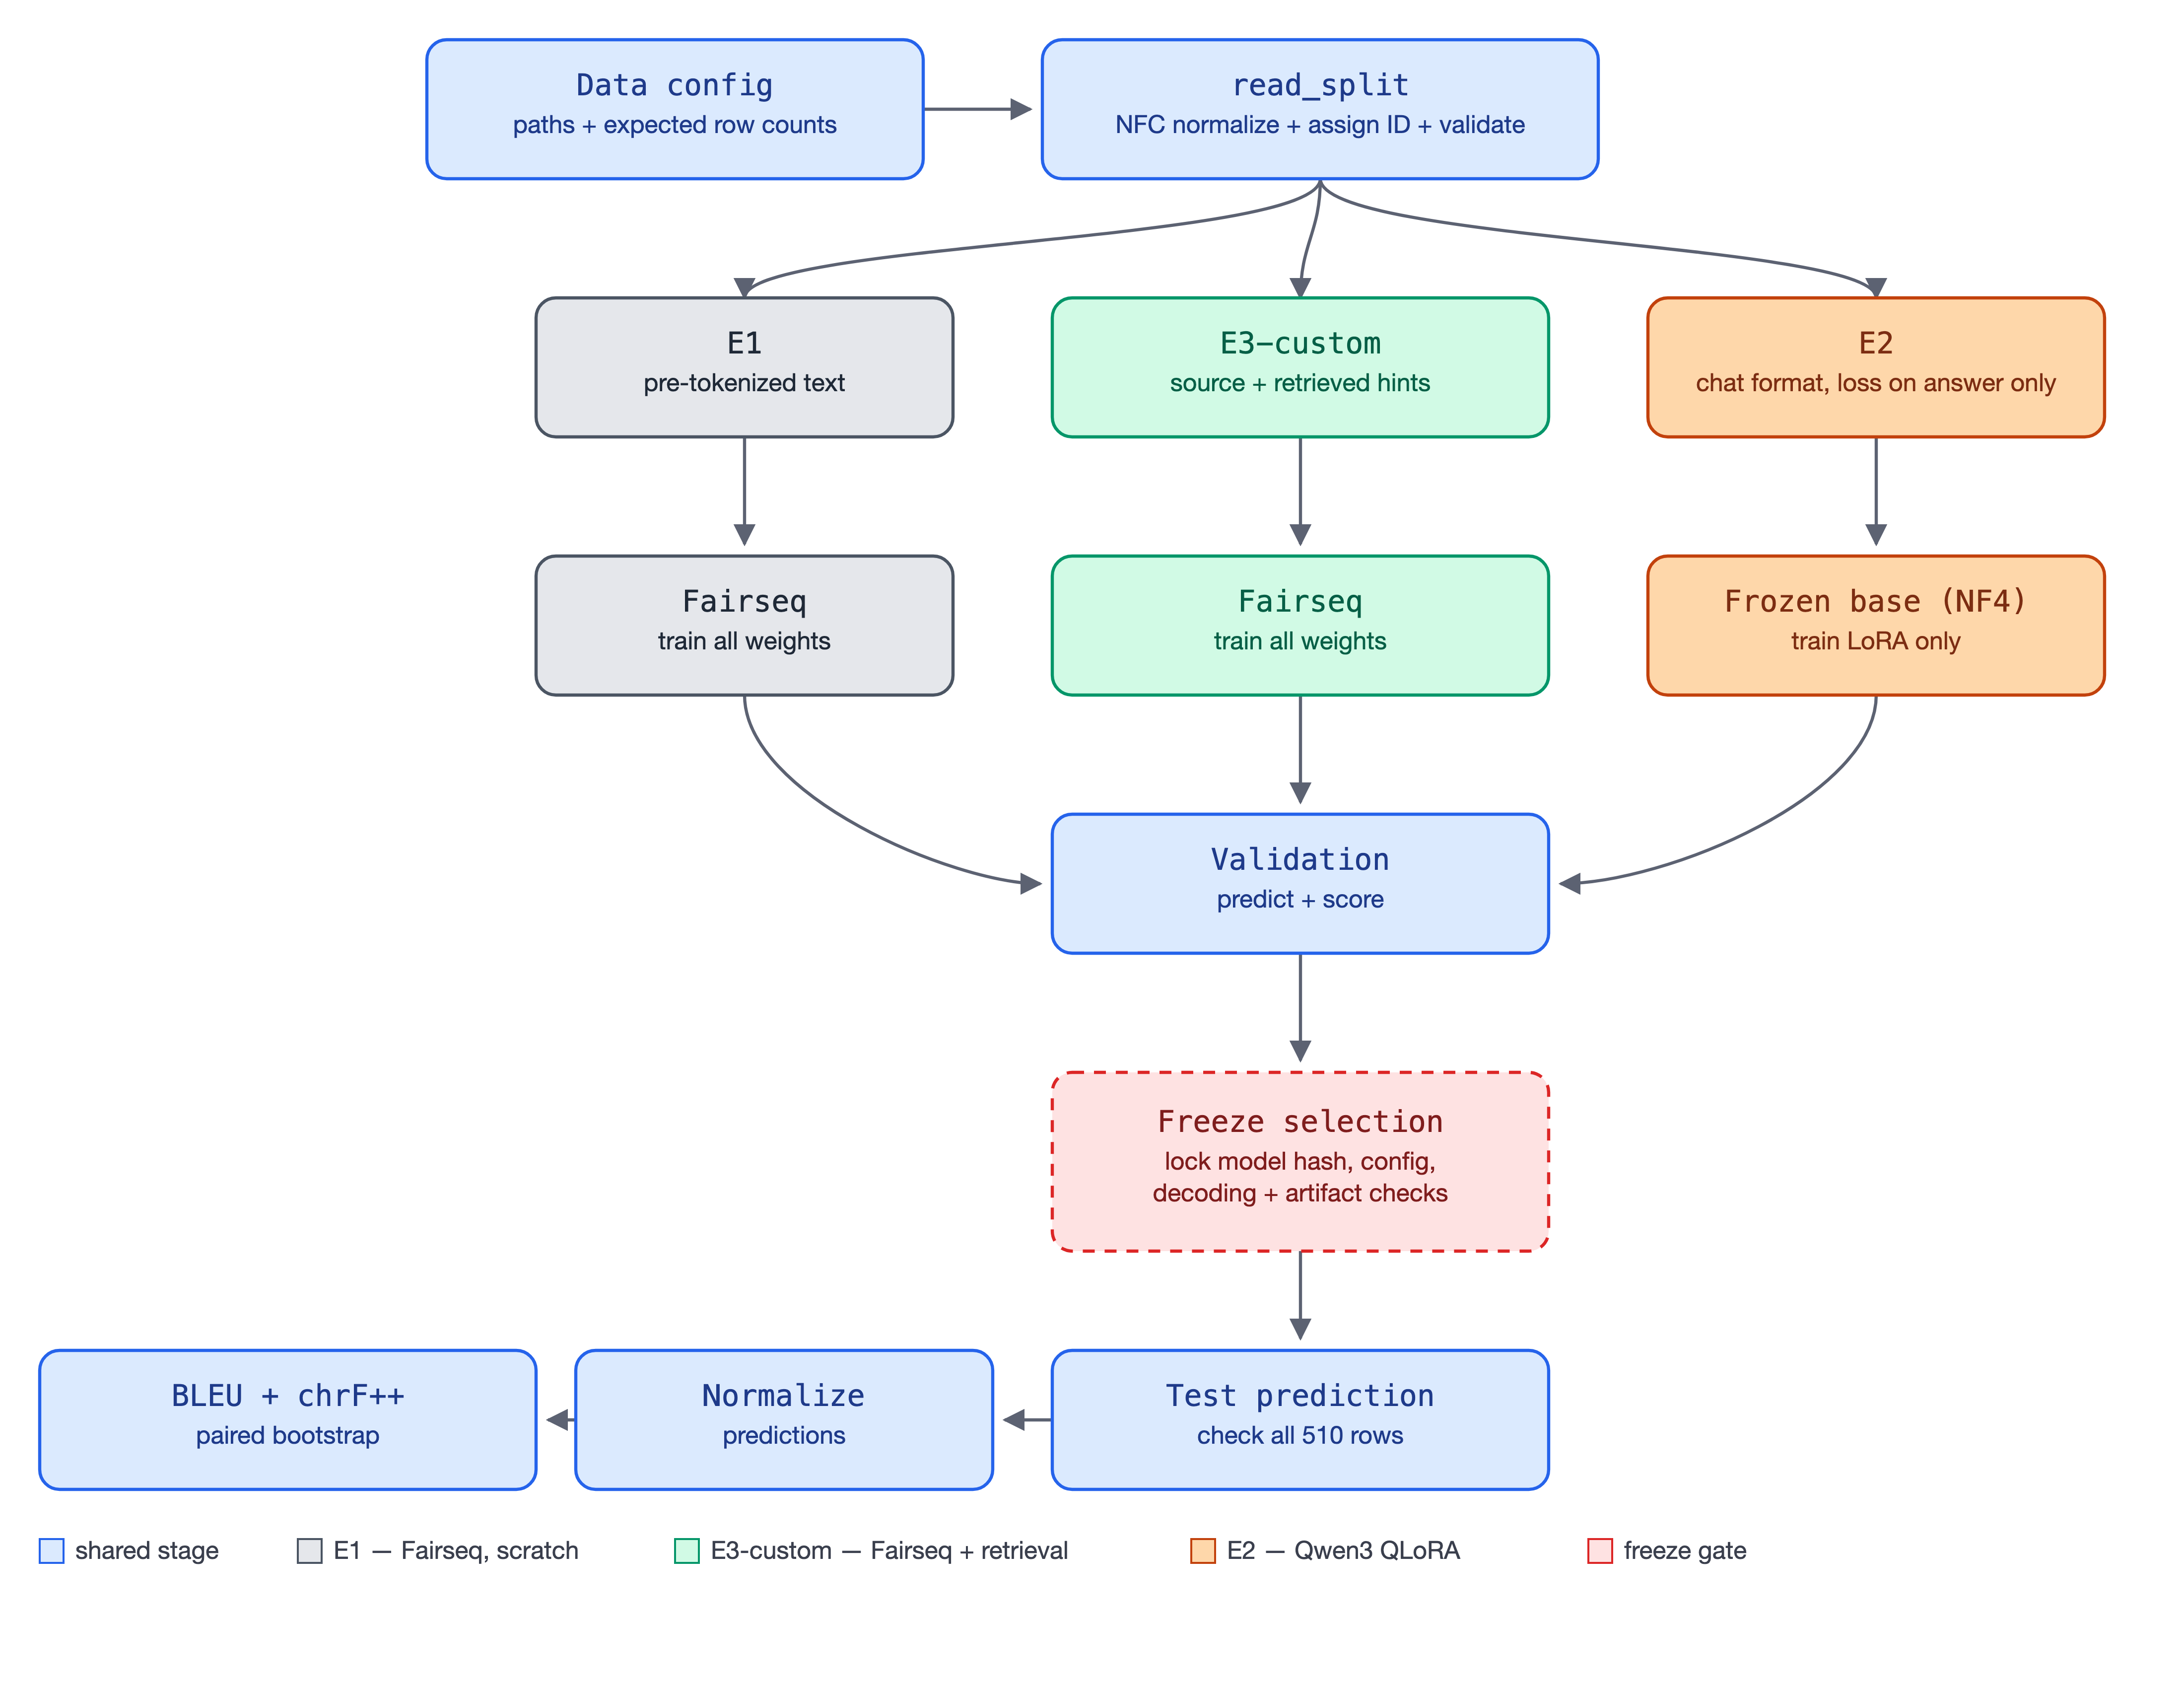
\includegraphics[width=\linewidth]{img/mt_pipeline.png}
  \caption{Tổng quan pipeline}
  \label{fig:pipeline}
\end{figure}

Ở đầu vào, cả ba thí nghiệm cùng đi qua một cấu hình dữ liệu và bước \texttt{read\_split}
duy nhất (mục 3.1): chuẩn hoá NFC, gộp khoảng trắng, gán định danh mẫu và kiểm tra toàn
vẹn số dòng. Từ đây, pipeline rẽ thành ba nhánh độc lập. \texttt{E1} giữ nguyên văn bản
đã tách token sẵn và huấn luyện toàn bộ trọng số một Transformer Fairseq từ đầu.
\texttt{E3-custom} đi theo đúng con đường Fairseq như \texttt{E1} nhưng bổ sung thêm
gợi ý Hán tự truy hồi vào câu nguồn trước khi huấn luyện — cũng huấn luyện toàn bộ
trọng số, chỉ khác ở dữ liệu đầu vào. \texttt{E2} tách khỏi con đường Fairseq hoàn toàn và chạy hoàn toàn dựa vào việc chúng ta thiết kế system prompt:
dữ liệu được đóng gói thành định dạng hội thoại với loss chỉ tính trên phần trả lời, và
chỉ một phần rất nhỏ tham số (adapter LoRA) được huấn luyện trên một mô hình nền đã
đóng băng và lượng tử hoá 4-bit.

Ba nhánh hội tụ trở lại ở một quy trình đánh giá dùng chung. Cả ba mô hình đều được
dùng để dự đoán và chấm điểm trên tập validation; kết quả này quyết định việc chốt
một cấu hình mô hình duy nhất cho mỗi thí nghiệm — khoá lại hash mô hình, cấu hình, cách
decode ra tiếng Hán để đảm bảo thí nghiệm có thể chạy lại với kết quả y hệt, và kiểm tra artifact trước khi chúng ta thực hiện dự đoán trên tập test. Dự đoán cuối cùng được chuẩn hoá về cùng một dạng chấm điểm (mục
3.6) trước khi tính BLEU và chrF++, và chênh lệch giữa các thí nghiệm được kiểm định bằng
paired bootstrap (mục 3.7).

\subsection{Dữ liệu và Tiền xử lý}

Trước khi dữ liệu song ngữ Việt--Hán văn cổ được đưa vào bất kỳ thí nghiệm nào, toàn bộ
ba phân hoạch (train, validation, test) đều đi qua một tầng tiền xử lý dùng chung, gồm
ba thành phần: (i) một bước \textit{chuẩn hoá văn bản} áp dụng đồng nhất cho cả hai phía
nguồn/đích; (ii) một bước \textit{đọc và kiểm tra toàn vẹn dữ liệu} chịu trách nhiệm gán
định danh mẫu và chặn đứng mọi lệch lạc về số dòng; và (iii) một tầng \textit{biểu diễn
văn bản đích dưới nhiều dạng} phục vụ ba mục đích khác nhau: huấn luyện, hiển thị, và
chấm điểm. Tầng tiền xử lý này được cài đặt trong \texttt{code/mt\_pipeline/normalize.py}
và \texttt{code/mt\_pipeline/data.py}, và là điểm khởi đầu chung cho cả ba thí nghiệm E1,
E2 và E3-custom trước khi mỗi thí nghiệm rẽ theo hướng chuẩn bị dữ liệu riêng của mình.

\subsubsection{Chuẩn hoá văn bản}

Hàm \texttt{normalize\_whitespace} được áp dụng cho cả câu nguồn tiếng Việt lẫn câu đích
Hán văn ngay khi đọc dữ liệu:
\begin{equation}
  \texttt{normalize\_whitespace}(s) = \mathrm{strip}\Big(\mathrm{collapse}_{\backslash s+ \to \text{"~"}}\big(\mathrm{NFC}(s)\big)\Big),
  \label{eq:normalize-whitespace}
\end{equation}
trong đó $s$ là chuỗi văn bản thô đọc từ tệp corpus, $\mathrm{NFC}(\cdot)$ là phép chuẩn
hoá Unicode theo dạng \textit{Normalization Form Canonical Composition},
$\mathrm{collapse}_{\backslash s+ \to \text{"~"}}(\cdot)$ là phép thay thế mọi chuỗi
khoảng trắng liên tiếp bằng đúng một dấu cách, và $\mathrm{strip}(\cdot)$ là phép cắt bỏ
khoảng trắng thừa ở hai đầu chuỗi.

Bước NFC là cần thiết vì tiếng Việt có dấu thanh và dấu phụ có thể được mã hoá theo hai
cách tương đương nhưng khác biểu diễn byte: dạng \textit{dựng sẵn} (một mã Unicode duy
nhất cho cả âm tiết có dấu) và dạng \textit{tổ hợp} (ký tự gốc cộng thêm một dấu kết hợp
riêng biệt). Lấy ví dụ như: chữ \texttt{"ả"} có thể là một mã Unicode duy nhất
\texttt{U+1EA3} (dạng dựng sẵn), hoặc là hai mã Unicode nối tiếp nhau
\texttt{"a" (U+0061) + dấu hỏi kết hợp (U+0309)} (dạng tổ hợp) — hai chuỗi byte hoàn
toàn khác nhau nhưng hiển thị giống hệt \texttt{"ả"}. Nếu không ép cả hai về cùng một
dạng, hai câu nhìn giống hệt nhau có thể bị xem là khác nhau khi so khớp chuỗi, dẫn tới
sai lệch khi gán định danh, kiểm tra trùng lặp hay tra cứu từ điển; sau khi qua
$\mathrm{NFC}(\cdot)$, cả hai đều quy về đúng một dạng \texttt{U+1EA3}.

Tương tự, với một dòng thô đọc từ tệp có khoảng trắng không nhất quán, chẳng hạn
\texttt{"Vua~~sai\textbackslash tngười"} (hai dấu cách liên tiếp rồi một tab), phép
$\mathrm{collapse}_{\backslash s+ \to \text{"~"}}(\cdot)$ gộp toàn bộ chuỗi khoảng trắng
đó lại thành đúng một dấu cách, cho ra \texttt{"Vua~sai~người"} — đảm bảo ranh giới token
luôn nhất quán bất kể tệp gốc chứa tab, xuống dòng thừa hay nhiều dấu cách liên tiếp do
lỗi định dạng khi xuất corpus.

\subsubsection{Đọc dữ liệu và kiểm tra toàn vẹn}

Hàm \texttt{read\_split} (\texttt{data.py}) là điểm đọc dữ liệu duy nhất của toàn bộ
pipeline. Với mỗi phân hoạch, hàm này: đọc đồng thời hai tệp nguồn và đích; buộc dừng
chương trình nếu số dòng hai phía không bằng nhau; buộc dừng chương trình nếu số dòng
đọc được khác với số dòng kỳ vọng \texttt{expected\_lines} khai báo trong cấu hình dữ
liệu; gán cho mỗi cặp câu một định danh duy nhất theo quy tắc
$\texttt{sample\_id} = \texttt{f"\{split\}-\{index:06d\}"}$; và áp dụng phép chuẩn hoá ở
Công thức~\ref{eq:normalize-whitespace} cho cả hai phía.

Lấy ví dụ như: với phân hoạch \texttt{train} và dòng thứ 42 (đếm từ 1), định danh mẫu
được gán là $\texttt{sample\_id} = \texttt{"train-000042"}$ — định danh này giữ nguyên
không đổi xuyên suốt pipeline, dùng để đối chiếu dự đoán với tham chiếu và để ghép cặp
đúng câu khi so sánh hai hệ thống ở mục 3.7. Về hai điều kiện hard-fail: giả sử tệp
nguồn tiếng Việt của tập train có 19.218 dòng nhưng tệp đích Hán văn chỉ có 19.217 dòng
(một dòng bị rơi mất do lỗi khi xuất tệp, hoặc một bản sửa tệp không đồng bộ giữa hai
phía) — \texttt{read\_split} sẽ dừng chương trình ngay lập tức với lỗi báo số dòng hai
phía không khớp, thay vì âm thầm ghép lệch câu nguồn với câu đích của dòng kế tiếp và để
lỗi đó lan vào toàn bộ quá trình huấn luyện mà không ai phát hiện. Tương tự, nếu cấu hình
khai báo \texttt{expected\_lines: 19218} cho tập train nhưng tệp thực tế chỉ có 19.000
dòng (ví dụ do tải nhầm một phiên bản corpus cũ hoặc bị cắt xén khi sao chép), hàm cũng
dừng ngay thay vì lặng lẽ huấn luyện trên một tập dữ liệu nhỏ hơn dự kiến. Hai điều kiện
hard-fail này đóng vai trò một cổng toàn vẹn dữ liệu, đảm bảo một tệp corpus bị hoán đổi
nhầm hoặc bị cắt xén không thể lọt vào một lượt chạy thực nghiệm mà không bị phát hiện
ngay từ bước đọc dữ liệu đầu tiên.

\subsubsection{Ba dạng biểu diễn của câu đầu ra}

Vì phía Hán văn được cung cấp sẵn dưới dạng tách ký tự, mỗi dòng dữ liệu đích cần được
biểu diễn dưới ba dạng khác nhau tuỳ mục đích sử dụng:

\begin{table}[H]
    \centering
    \small
    \caption{Ba dạng biểu diễn của câu đích Hán văn}
    \label{tab:three-text-forms}
    \begin{tabularx}{\textwidth}{@{}
        >{\raggedright\arraybackslash}p{0.26\textwidth}
        >{\raggedright\arraybackslash}X
        >{\raggedright\arraybackslash}X@{}}
        \toprule
        \textbf{Dạng} & \textbf{Định nghĩa} & \textbf{Dùng cho} \\
        \midrule
        \texttt{reference\_tokenized} & dòng gốc đã chuẩn hoá khoảng trắng & mục tiêu huấn luyện/đánh giá của Fairseq \\
        \texttt{reference} & \texttt{detokenize\_chinese}: nối ký tự, bỏ khoảng trắng & câu tham chiếu người đọc; mục tiêu huấn luyện của E2 \\
        \texttt{reference\_scored} & \texttt{score\_form\_chinese}: tách lại từng ký tự, nối bằng một dấu cách & đầu vào chấm điểm BLEU/chrF++ \\
        \bottomrule
    \end{tabularx}
\end{table}

Về mặt hình thức:
$$
\texttt{reference} = \mathrm{join}_{\varnothing}(\texttt{reference\_tokenized})
$$
còn
$$\texttt{reference\_scored} = \mathrm{join}_{\text{"~"}}\big(\mathrm{split}_{\text{codepoint}}(\texttt{reference})\big)$$
— tức \texttt{reference\_scored} là một phép tách--gộp--tách lại đi qua dạng không
khoảng trắng.

Lấy ví dụ như: với \texttt{reference\_tokenized} là \texttt{"如 使 越 人"}, áp dụng
\texttt{detokenize\_chinese} cho ra \texttt{reference} = \texttt{"如使越人"} (đã bỏ hết
khoảng trắng). Từ \texttt{reference} này, áp dụng tiếp \texttt{score\_form\_chinese} —
tách lại thành từng ký tự Unicode riêng lẻ rồi chèn một dấu cách giữa mỗi ký tự — cho ra
\texttt{reference\_scored} = \texttt{"如 使 越 人"}, \textbf{trùng khớp tuyệt đối} với
\texttt{reference\_tokenized} ban đầu. Kết quả này không phải ngẫu nhiên: nó minh hoạ
chính xác ý nghĩa của phép round-trip — đi một vòng qua dạng không khoảng trắng rồi tách
trở lại, ta thu được đúng dạng ban đầu, chứng tỏ không mất thông tin gì trong quá trình.
Bước tách--gộp--tách lại này được áp dụng như nhau cho \textit{mọi} hệ thống, kể cả những
hệ thống không tự nhiên sinh ra dạng tách-ký-tự (như \texttt{E2}, vốn sinh Hán văn liền
mạch giống hệt dạng \texttt{reference}): nhờ vậy, dự đoán của cả ba thí nghiệm đều được
ép về cùng một chuẩn (một Hán tự = một token) trước khi đưa vào chấm điểm, đảm bảo phép
so sánh BLEU/chrF++ công bằng dù các hệ thống có định dạng đầu ra thô khác nhau.

Phép round-trip này chỉ không mất thông tin khi mọi token gốc trong corpus đúng là một
codepoint duy nhất; điều kiện này đã được xác minh thực nghiệm trên toàn bộ 20.238 dòng
của cả ba phân hoạch, không có ngoại lệ. Việc tách riêng ba dạng biểu diễn này là điều
kiện cần để các chỉ số đánh giá (mục 3.6) được định nghĩa nhất quán giữa các thí nghiệm
có định dạng đầu ra khác nhau.

\subsubsection{Chính sách không dùng subword}

Khi xây dựng từ điển cho Fairseq, ngưỡng tần suất tối thiểu được đặt bằng 1 ở cả hai phía
(\texttt{--thresholdsrc 1 --thresholdtgt 1}), nghĩa là không áp dụng bất kỳ thuật toán
ghép subword nào (không BPE, không WordPiece) và toàn bộ từ vựng xuất hiện trong tập
train đều được giữ nguyên. Kết quả: từ điển tiếng Việt có 3.616 loại từ (word-level), từ
điển Hán văn có 5.392 loại ký tự (character-level). Lựa chọn này có chủ đích: ghép các
chuỗi Hán tự liên tiếp thành đơn vị subword theo thống kê đồng xuất hiện chỉ đáng tin cậy
khi học trên một corpus đủ lớn; với một corpus nhỏ, phạm vi hẹp như \textit{Đại Việt sử
ký toàn thư}, một mô hình subword riêng có nguy cơ tạo ra các đơn vị ghép không ổn định,
phụ thuộc mạnh vào các mẫu câu lặp lại đặc trưng của corpus hơn là phản ánh đúng cấu trúc
ngôn ngữ. Cái giá phải trả: từ điển cố định không sinh được những ký tự chỉ xuất hiện ở
tập giữ riêng — 34 token đích ngoài từ điển ở validation, 45 ở test.

\subsection{Thí nghiệm 1 (E1): Transformer huấn luyện từ đầu}

\subsubsection{Kiến trúc Transformer}

Transformer~\cite{vaswani2017attention} là một kiến trúc mạng nơ-ron cho bài toán chuỗi
sang chuỗi, gồm hai khối \textit{encoder} và \textit{decoder}, xây dựng hoàn toàn từ cơ
chế \textit{self-attention} thay vì hồi quy (RNN/LSTM) hay tích chập (CNN). Thành phần
cốt lõi là \textit{scaled dot-product attention}:
\begin{equation}
  \mathrm{Attention}(Q,K,V) = \mathrm{softmax}\!\left(\frac{QK^{\top}}{\sqrt{d_k}}\right)V,
  \label{eq:e1-attention}
\end{equation}
trong đó $Q$ (query), $K$ (key) và $V$ (value) là ba phép chiếu tuyến tính khác nhau của
cùng một biểu diễn đầu vào; tích $QK^{\top}$ đo độ tương đồng giữa mỗi cặp vị trí, chia
cho $\sqrt{d_k}$ để tránh giá trị quá lớn làm softmax bão hoà; kết quả softmax là trọng số
attention dùng để lấy tổ hợp trọng số của $V$. \textit{Multi-head attention} chạy song
song $h$ head attention trên $h$ phép chiếu khác nhau rồi nối kết quả lại, giúp mô hình
chú ý đồng thời tới nhiều loại quan hệ khác nhau giữa các vị trí trong câu.

Kiến trúc này phù hợp với dịch máy vì hai lý do: self-attention cho phép mỗi vị trí chú
ý trực tiếp tới mọi vị trí khác qua một bước duy nhất (giảm vanishing gradient với câu
dài, hữu ích khi trật tự từ giữa tiếng Việt và Hán văn cổ có thể lệch xa nhau); và vì
không có hồi quy tuần tự như dạng cấu trúc RNN hay LSTM, toàn bộ chuỗi input vào trong mô hình sẽ được xử lý song song khi huấn luyện.

\subsubsection{Fairseq}

Fairseq~\cite{ott2019fairseq} là một toolkit huấn luyện mô hình chuỗi mã nguồn mở, xây
dựng trên PyTorch. Fairseq cung cấp cài đặt tham chiếu cho Transformer cùng hạ tầng huấn
luyện/giải mã chuẩn hoá (gom batch theo token, checkpoint, beam search,v.v...). \texttt{E1}
dùng Fairseq thay vì tự cài đặt lại, để bám sát một cài đặt chuẩn đã được kiểm chứng rộng
rãi, tập trung nỗ lực vào lựa chọn dữ liệu/cấu hình thay vì hiện thực hoá mô hình.

\subsubsection{Cấu hình và hàm mục tiêu}

\texttt{E1} dùng Transformer encoder--decoder tiêu chuẩn: sáu lớp mỗi khối, biểu diễn
512 chiều, feed-forward 2.048 chiều, tám attention head, dropout 0,1. Embedding đầu vào
và ma trận chiếu đầu ra của decoder chia sẻ trọng số. Mô hình có 67.652.608 tham số, tối
ưu từ đầu, không qua fine-tuning. Ở phía tiếng Việt, đơn vị đầu vào là token có sẵn trong
corpus; ở phía Hán văn, mỗi ký tự là một token, theo đúng chính sách không dùng BPE đã
nêu ở mục 3.1.

Với câu đích $y_{1:T}$, \texttt{E1} tối thiểu hoá hàm cross-entropy có label smoothing
$\varepsilon=0{,}1$:
\begin{equation}
  \mathcal{L}_{\mathrm{E1}}
  = -\sum_{t=1}^{T}\left[(1-\varepsilon)\log p(y_t\mid y_{<t},x)
  + \frac{\varepsilon}{|V|}\sum_{v\in V}\log p(v\mid y_{<t},x)\right].
  \label{eq:e1-loss}
\end{equation}
Bộ tối ưu Adam dùng $\beta=(0{,}9,\,0{,}998)$, learning rate cực đại $5\times10^{-4}$ và
lịch \texttt{inverse\_sqrt} sau 8.000 update warmup. Mỗi GPU nhận tối đa 1.000 token;
\texttt{update\_freq=4} tạo batch hiệu dụng khoảng 4.000 token. Huấn luyện chạy ở fp16
trên một GPU, giới hạn 50.000 update hoặc 500 epoch, patience 20 theo BLEU validation.
Cần lưu ý checkpoint được báo cáo đã \textit{warm-start}: nạp lại trọng số từ một lần
chạy trước bị gián đoạn ở epoch 5 (update 579), sau đó tiếp tục và early-stop ở epoch
171 (24.791 update) — một hạn chế về khả năng tái lập từ một lần chạy sạch cần ghi nhận.

\subsubsection{Giải mã bằng beam search}

Thay vì luôn chọn token xác suất cao nhất ở mỗi bước (\textit{greedy decoding}, dễ mắc
kẹt vào chuỗi con tối ưu cục bộ), \texttt{E1} dùng beam search với $B=7$: duy trì đồng
thời $B$ giả thuyết có tổng log-xác suất cao nhất, mở rộng mỗi giả thuyết bằng mọi token
kế tiếp, chỉ giữ lại $B$ chuỗi tốt nhất cho bước sau, lặp tới khi mọi beam kết thúc câu
hoặc chạm giới hạn độ dài.

Vì tổng log-xác suất giảm dần theo số token, một chuỗi ngắn hơn sẽ có điểm cao hơn một
cách giả tạo nếu không hiệu chỉnh. Fairseq chuẩn hoá điểm theo độ dài với hệ số length
penalty $\alpha$:
\begin{equation}
  \mathrm{score}(y) = \frac{1}{|y|^{\alpha}}\sum_{t=1}^{|y|}\log p(y_t\mid y_{<t},x),
  \label{eq:e1-beam-score}
\end{equation}
\texttt{E1} dùng $\alpha=1{,}0$ — điểm cuối chính là log-xác suất trung bình mỗi token,
không thiên vị thêm ngoài chuẩn hoá độ dài tự nhiên. Độ dài đích tối đa giới hạn theo
$1{,}2|x|+10$ token, với $|x|$ là độ dài câu nguồn — ngăn mô hình sinh chuỗi kéo dài vô
hạn định với câu nguồn dài. Các giá trị beam, length penalty và giới hạn độ dài này được
cố định trước khi chạy, không phải kết quả tìm kiếm siêu tham số.


\subsubsection{Ví dụ minh hoạ toàn bộ quy trình}

Để cụ thể hoá các khái niệm trên, xét một câu ví dụ minh hoạ (không phải câu thật trong
corpus): câu nguồn tiếng Việt \texttt{"Vua sai sứ sang nước Tống"} cần dịch thành Hán
văn cổ tương ứng "王 遣 使 如 宋".

\paragraph{Input đưa vào mô hình.} Vì phía tiếng Việt đã được tách token sẵn trong
corpus, câu nguồn là chuỗi 6 token \texttt{["Vua","sai","sứ","sang","nước","Tống"]};
câu đích Hán văn, tách theo ký tự, là chuỗi 5 token ["王","遣","使","如","宋"]. Sau bước
tiền xử lý ở mục 3.1 (chuẩn hoá NFC + gộp khoảng trắng), hai chuỗi này được ghi ra file
văn bản thô (\texttt{text/train.vi}, \texttt{text/train.zh}). Mô hình Transformer không
đọc trực tiếp chuỗi ký tự — mỗi token được ánh xạ sang một chỉ số nguyên duy nhất trong
từ điển tương ứng (\texttt{dict.vi.txt} cho phía nguồn, \texttt{dict.zh.txt} cho phía
đích): ví dụ \texttt{"Vua"} $\to$ id 42, \texttt{"sai"} $\to$ id 803, chữ "王" $\to$ id
187, chữ "遣" $\to$ id 1204, v.v. Chuỗi chỉ số này (\emph{không phải} chuỗi ký tự) mới là
đầu vào số học thực sự được đưa vào embedding layer của encoder/decoder.

\paragraph{Fairseq construct những gì.} Bước nhị phân hoá chạy đúng một lệnh:
\begin{quote}\ttfamily\small
fairseq-preprocess --source-lang vi --target-lang zh \\
\quad --trainpref text/train --validpref text/valid --testpref text/test \\
\quad --destdir data-bin --thresholdsrc 1 --thresholdtgt 1 --workers 4
\end{quote}
Lệnh này quét toàn bộ \texttt{text/train.\{vi,zh\}}, xây hai từ điển
\texttt{dict.vi.txt}/\texttt{dict.zh.txt} (mỗi dòng là một token kèm tần suất xuất hiện,
sắp theo tần suất giảm dần), rồi mã hoá mọi câu của cả ba phân hoạch thành cặp tệp nhị
phân \texttt{.bin}/\texttt{.idx} (mảng chỉ số nguyên nén, đọc nhanh hơn nhiều so với parse
văn bản mỗi epoch). Kết quả nằm trong thư mục \texttt{data-bin/}, là đầu vào duy nhất cho
bước huấn luyện tiếp theo — tức Fairseq không "học" trực tiếp trên file text, mà học trên
biểu diễn nhị phân đã được lập chỉ mục này. Bước huấn luyện sau đó gọi
\texttt{fairseq-train} trên \texttt{data-bin/} với toàn bộ cờ kiến trúc/tối ưu đã liệt kê
ở mục trên (\texttt{--arch transformer --encoder-layers 6 ... --lr 5e-4 ...}), ghi
checkpoint định kỳ vào \texttt{checkpoint\_dir}.

\paragraph{Output nhìn như thế nào.} Khi giải mã (dùng \texttt{fairseq-generate} trên
checkpoint tốt nhất), với mỗi câu, công cụ in ra 4 dòng gắn theo chỉ số câu, ví dụ với
câu thứ 3 (định dạng \texttt{S-}/\texttt{T-}/\texttt{H-}/\texttt{D-} là quy ước gốc của
Fairseq, phần văn bản Hán/Việt giữ nguyên font thường vì font monospace không có glyph
chữ Hán):

\begin{quote}\small
\texttt{S-3}\quad Vua sai sứ sang nước Tống \\
\texttt{T-3}\quad 王 遣 使 如 宋 \\
\texttt{H-3}\quad $-0{,}3821$\quad 王 遣 使 如 宋 \\
\texttt{D-3}\quad $-0{,}3821$\quad 王 遣 使 如 宋
\end{quote}
trong đó \texttt{S} là câu nguồn, \texttt{T} là câu đích tham chiếu, \texttt{H} là giả
thuyết (hypothesis) tốt nhất cùng log-xác suất trung bình mỗi token của nó (chính là
Công thức~\ref{eq:e1-beam-score}), và \texttt{D} là bản detokenize của \texttt{H} (ở đây
trùng nhau vì không có hậu xử lý detokenize riêng phía Fairseq). Pipeline chỉ đọc dòng
\texttt{H-}, tách ra được chuỗi ký tự "王 遣 使 如 宋" — đây chính là
\texttt{reference\_tokenized}-dạng của dự đoán. Từ đó, hai phép biến đổi ở mục 3.1 được
áp dụng: \texttt{detokenize\_chinese} cho ra \texttt{prediction} = "王遣使如宋" (dạng
người đọc), rồi \texttt{score\_form\_chinese} cho ra \texttt{prediction\_scored} = "王 遣
使 如 宋" — dạng dùng để chấm BLEU/chrF++ ở mục 3.6.

\paragraph{Beam search decode nhìn như thế nào.} Để dễ minh hoạ, xét beam size $B=3$ (trong bài dùng $B=3$)

\begin{table}[H]
\centering\small
\caption{Minh hoạ hai bước đầu của beam search ($B=3$)}
\begin{tabular}{clc}
\toprule
\textbf{Bước} & \textbf{3 giả thuyết được giữ lại} & \textbf{Log-xác suất cộng dồn} \\
\midrule
1 & "王" & $-0{,}10$ \\
  & "帝" & $-0{,}90$ \\
  & "上" & $-1{,}20$ \\
\midrule
2 & "王 遣" & $-0{,}15$ \\
  & "王 命" & $-0{,}90$ \\
  & "帝 遣" & $-1{,}20$ \\
\bottomrule
\end{tabular}
\end{table}

Ở bước 1, mô hình cho ra phân phối xác suất trên toàn bộ từ điển đích cho token đầu
tiên; ba token có log-xác suất cao nhất được giữ làm 3 giả thuyết ban đầu. Ở bước 2, cả
ba giả thuyết đều được mở rộng bằng \emph{mọi} token tiếp theo có thể (không chỉ 3 token
trong bảng — bảng chỉ hiện kết quả sau khi lọc), tạo ra rất nhiều chuỗi ứng viên độ dài
2; trong số đó, chỉ 3 chuỗi có tổng log-xác suất cộng dồn cao nhất được giữ lại cho bước
3 — ở đây là "王 遣", "王 命" và "帝 遣", còn mọi mở rộng khác của "上" và các mở rộng kém
hơn của "帝" bị loại bỏ hoàn toàn dù tại bước 1 "帝" từng lọt vào top-3. Quá trình lặp lại
như vậy cho đến khi cả 3 giả thuyết sinh token kết thúc câu hoặc chạm giới hạn
$1{,}2|x|+10$ token; giả thuyết có điểm đã chuẩn hoá độ dài (Công thức~\ref{eq:e1-beam-score})
cao nhất trong số các giả thuyết đã kết thúc được chọn làm câu dịch cuối cùng — chính là
dòng \texttt{H-3} ở trên.

\subsection{Thí nghiệm 2 (E2): Qwen3-8B với QLoRA}

\subsubsection{Mô hình ngôn ngữ lớn và Qwen3-8B}

Khác với \texttt{E1} huấn luyện Transformer từ đầu, \texttt{E2} tinh chỉnh một mô hình
ngôn ngữ lớn đã tiền huấn luyện: \texttt{Qwen3-8B}~\cite{qwenteam2025qwen3}, một mô hình
\textit{decoder-only} khoảng 8 tỷ tham số. Một LLM decoder-only mô hình hoá xác suất
chuỗi đích $y$ tự hồi quy, có điều kiện trên chuỗi nhắc $x$:
\begin{equation}
  P(y \mid x) = \prod_{t=1}^{T} p\bigl(y_t \mid x,\, y_{<t}\bigr).
  \label{eq:e2-causal-lm}
\end{equation}
$x$ là chuỗi nhắc (system instruction cùng câu nguồn tiếng Việt), $y_{1:T}$ là bản dịch
Hán văn cổ sinh ra. Mỗi thừa số được tính bằng cách cho tiền tố đi qua các khối
self-attention xếp chồng với \textit{causal mask}: điểm attention từ vị trí $t$ đến mọi
vị trí $>t$ bị gán $-\infty$ trước softmax, nên vị trí $t$ chỉ "nhìn thấy" chính nó và
các vị trí trước.

Lý do chọn tinh chỉnh LLM có sẵn thay vì huấn luyện từ đầu như \texttt{E1}: với
\texttt{E1}, mọi tri thức ngôn ngữ và dịch thuật phải học hoàn toàn từ 19.218 cặp câu.
\texttt{Qwen3-8B} đã tiền huấn luyện trên kho ngữ liệu khổng lồ, nhiều khả năng gồm cả
tiếng Việt, Hán văn hiện đại và một phần Hán văn cổ, nên đã có sẵn hiểu biết đáng kể về
từ vựng/ngữ pháp/văn phong hai ngôn ngữ trước khi tiếp xúc dữ liệu đề tài. So sánh
\texttt{E1} với \texttt{E2} là phép kiểm định cho giả thuyết: tri thức tiền huấn luyện
kết hợp phương pháp tinh chỉnh tiết kiệm tham số có bù đắp được quy mô ngữ liệu song ngữ
nhỏ hay không.

\subsubsection{LoRA và QLoRA}

Tinh chỉnh toàn bộ 8 tỷ tham số trên chỉ 19.218 câu vừa tốn bộ nhớ vừa dễ overfitting.
\texttt{E2} dùng LoRA~\cite{hu2021lora}: giữ nguyên (đóng băng) ma trận trọng số
$W \in \mathbb{R}^{d\times k}$, chỉ học cập nhật hạng thấp $\Delta W = BA$, với
$B\in\mathbb{R}^{d\times r}$, $A\in\mathbb{R}^{r\times k}$, $r \ll \min(d,k)$:
\begin{equation}
  h = Wx + \frac{\alpha}{r}\,BAx.
  \label{eq:e2-lora}
\end{equation}
$r$ (rank) là chiều "cổ chai" của cập nhật, quyết định số tham số mới ($r(d+k)$ thay vì
$d\times k$); đề tài dùng $r=16$. $\alpha$ là hệ số tỷ lệ cố định tách độ lớn cập nhật
khỏi giá trị $r$; dùng $\alpha=32$, cho tỷ lệ $\alpha/r=2$. \texttt{target\_modules=all-linear}
nghĩa là mọi lớp tuyến tính trong các khối Transformer đều được gắn một cặp $(A,B)$
riêng. Tại khởi tạo $B=0$ nên $\Delta W=0$, mô hình thích ứng ban đầu giống hệt mô hình
nền; chỉ $A,B$ được huấn luyện.

QLoRA~\cite{dettmers2023qlora} bổ sung lượng tử hoá phần trọng số nền đã đóng băng:
\textbf{NF4} (4-bit NormalFloat) đặt 16 mức lượng tử tại các phân vị của phân phối chuẩn
thay vì chia đều, tối ưu cho trọng số có phân phối gần chuẩn; \textbf{double
quantization} lượng tử hoá thêm chính các hằng số tỷ lệ; \textbf{compute dtype fp16}
giải lượng tử tức thời chỉ để nhân ma trận; \textbf{paged optimizer}
(\texttt{paged\_adamw\_8bit}) dùng phân trang bộ nhớ hợp nhất để tránh hết bộ nhớ. Kết
quả: khoảng 8 tỷ tham số nền chỉ chiếm khoảng một phần tư dung lượng so với fp16, trong
khi chỉ các ma trận LoRA — một phần rất nhỏ — thực sự được huấn luyện.

\subsubsection{Biểu diễn dữ liệu và hàm mất mát}

Khác \texttt{E1}/\texttt{E3-custom} dùng \texttt{reference\_tokenized} làm đích,
\texttt{E2} dùng \texttt{reference} (đã detokenize) — mô hình học sinh Hán văn tự nhiên,
không phải chuỗi cách nhau bởi khoảng trắng. Mỗi mẫu được dựng thành hội thoại hai lượt
(system instruction + câu nguồn), mã hoá hai lần qua \texttt{apply\_chat\_template} —
một lần chỉ tiền tố, một lần gồm cả câu trả lời — và khẳng định chuỗi đầy đủ bắt đầu
đúng bằng chuỗi tiền tố (kiểm tra an toàn chống lệch mask). Nhãn huấn luyện:
\begin{equation}
  \text{label}_i =
  \begin{cases}
    -100, & i < |P| \\
    \text{token}_i, & i \ge |P|
  \end{cases}
  \label{eq:e2-loss-mask}
\end{equation}
với $P$ là chuỗi token tiền tố. Giá trị $-100$ khiến cross-entropy bỏ qua vị trí đó — loss
chỉ tính trên token bản dịch. Nhiều mẫu hoàn chỉnh được đóng gói (packing) thành cửa sổ
768 token sau xáo trộn có seed; 19.218 mẫu đóng gói thành 2.903 chuỗi huấn luyện.

\subsubsection{Huấn luyện}

Tối ưu \texttt{paged\_adamw\_8bit}, lr $2\times10^{-4}$, lịch cosine, warmup 0,05,
weight decay 0,01, grad-norm clip 1,0. Batch hiệu dụng: 1 mẫu/thiết bị $\times$ 16 bước
tích luỹ gradient, 3 epoch (546 bước), fp16. Checkpoint triển khai là checkpoint có
\texttt{eval\_loss} thấp nhất, ở bước 400 (khoảng epoch 2,2/3) — không phải cuối huấn
luyện — được khôi phục (\texttt{load\_best\_model\_at\_end}) trước khi lưu.

\subsubsection{Giải mã}

Beam search với beam $=4$, tất định (\texttt{do\_sample=false}): luôn chọn tiếp tục có
xác suất tích luỹ cao nhất, không sampling. Số token tối đa thích ứng theo độ dài nguồn:
$\min(512,\ \lceil 2\times L_{\text{src}}\rceil + 32)$. Chuỗi nhắc khi giải mã dựng lại
giống hệt lúc huấn luyện, đảm bảo không lệch hình dạng giữa hai giai đoạn.

\subsubsection{Ví dụ minh hoạ toàn bộ quy trình}

\paragraph{Input và chuỗi nhắc.} Với cùng câu ví dụ "Vua sai sứ sang nước Tống" (đích:
"王遣使如宋", đã detokenize, không khoảng trắng), \texttt{E2} dựng hội thoại hai lượt:
\begin{quote}\small
\textbf{system}: Bạn là hệ thống dịch văn bản lịch sử. Hãy dịch câu tiếng Việt sang Hán
văn cổ. Chỉ trả về bản dịch Hán văn, không giải thích. \\
\textbf{user}: Dịch sang Hán văn cổ:\newline Vua sai sứ sang nước Tống
\end{quote}
Chuỗi này được mã hoá hai lần: \emph{tiền tố} (chỉ system+user, cộng thêm token báo hiệu
lượt trả lời sắp tới) và \emph{đầy đủ} (tiền tố cộng thêm câu trả lời "王遣使如宋"). Giả
sử (số minh hoạ) tiền tố mã hoá thành $|P|=38$ token, và chuỗi đầy đủ mã hoá thành 43
token (5 token còn lại ứng với 5 ký tự bản dịch). Mã nguồn khẳng định
\texttt{full\_ids[:38] == prefix\_ids} — nếu không đúng (ví dụ do thay đổi chat template
làm lệch điểm cắt), quá trình huấn luyện dừng ngay thay vì âm thầm tính loss sai vị trí.

\paragraph{Nhãn huấn luyện (loss mask).} Áp dụng Công thức~\ref{eq:e2-loss-mask} với
$|P|=38$: 38 vị trí đầu (toàn bộ system + user) nhận nhãn $-100$, chỉ 5 vị trí cuối (ứng
với 5 ký tự "王","遣","使","如","宋") mang token ID thật để tính loss:
\begin{quote}\small
\texttt{labels = [-100, -100, ..., -100,} (38 lần)\texttt{, id("王"), id("遣"), id("使"), id("如"), id("宋")]}
\end{quote}
Mô hình không bao giờ bị phạt vì "đoán sai" phần chỉ dẫn hệ thống hay câu nguồn — điều
đó vốn đã cho sẵn, chỉ có 5 token cuối mới đóng góp vào gradient.

\paragraph{LoRA vận hành cụ thể ra sao.} Xét ví dụ số học thu nhỏ (không phải kích thước
thật của Qwen3-8B) để thấy Công thức~\ref{eq:e2-lora} tính toán thế nào: giả sử một ma
trận trọng số $W \in \mathbb{R}^{4\times4}$ trong một lớp tuyến tính, hạng $r=2$ (thay vì
16 thật), và tỷ lệ $\alpha/r = 2$ (giữ đúng tỷ lệ $32/16=2$ của cấu hình thật):
\[
W=\begin{pmatrix}1&0&0&1\\0&1&1&0\\1&1&0&0\\0&0&1&1\end{pmatrix},\quad
A=\begin{pmatrix}1&0&1&0\\0&1&0&1\end{pmatrix},\quad
B=\begin{pmatrix}1&0\\0&1\\1&1\\0&0\end{pmatrix}.
\]
Với đầu vào $x=(1,1,0,0)^\top$: $Wx=(1,1,2,0)^\top$ (phần đóng góp từ mô hình nền, không
đổi khi huấn luyện). Thay vì nhân trực tiếp $BA$ (ra một ma trận $4\times4$ đầy đủ), LoRA
tính qua hai bước rẻ hơn nhiều: $Ax=(1,1)^\top$ (chỉ 2 chiều), rồi
$B(Ax)=(1,1,2,0)^\top$. Nhân với tỷ lệ $\alpha/r=2$:
$\frac{\alpha}{r}B(Ax) = (2,2,4,0)^\top$. Kết quả cuối:
\[
h = Wx + \frac{\alpha}{r}BAx = (1,1,2,0)^\top + (2,2,4,0)^\top = (3,3,6,0)^\top.
\]
Điểm mấu chốt về hiệu quả bộ nhớ/tính toán: LoRA không bao giờ cần dựng ma trận $4\times4$
đầy đủ của $BA$, chỉ cần hai phép nhân nhỏ qua chiều $r$. Ở quy mô thật ($d=k=4096$ chẳng
hạn, một bậc kích thước hợp lý cho các lớp tuyến tính của một mô hình 8 tỷ tham số), một
ma trận $W$ đầy đủ có $4096 \times 4096 \approx 16{,}8$ triệu tham số; với $r=16$, cặp
$A,B$ chỉ cần $16\times(4096+4096) \approx 131$ nghìn tham số — ít hơn khoảng 128 lần.
Vì \texttt{target\_modules=all-linear} áp dụng điều này cho \emph{mọi} lớp tuyến tính
trong mạng, mức tiết kiệm này nhân lên trên toàn bộ 8 tỷ tham số nền, giải thích vì sao
chỉ một phần rất nhỏ thực sự cần huấn luyện và lưu trữ ở độ chính xác cao.

\paragraph{Giải mã.} Với câu nguồn "Vua sai sứ sang nước Tống" giả sử mã hoá thành
$L_{\text{src}}=9$ token (theo tokenizer của Qwen3), giới hạn sinh token thích ứng là
$\min(512,\ \lceil 2\times 9\rceil + 32) = \min(512, 50) = 50$ token — đủ rộng cho một
bản dịch 5 ký tự nhưng không cho phép mô hình sinh tràn lan nếu lặp vòng. Vì
\texttt{do\_sample=false}, quá trình beam search ở đây hoàn toàn tất định: với cùng một
checkpoint và cùng một câu nguồn, chạy lại nhiều lần luôn cho ra đúng một kết quả — khác
với sinh văn bản có \textit{sampling} (nơi mỗi lần chạy có thể ra kết quả khác nhau do
yếu tố ngẫu nhiên trong việc chọn token).


\subsection{Thí nghiệm 3 (E3-custom): Fairseq với truy hồi tri thức nguồn}

Về kiến trúc, hàm mục tiêu, bộ tối ưu và giải mã, \texttt{E3-custom} hoàn toàn giống
\texttt{E1} (mục 3.3). Khác biệt duy nhất là một can thiệp \textit{chỉ ở tiền xử lý}:
trước khi mã hóa nhị phân, câu nguồn được bổ sung một danh sách Hán tự gợi ý truy hồi từ
một từ điển tri thức có cấu trúc.

Cần định vị đúng kỹ thuật này: đây không phải RAG truy hồi đoạn văn bằng embedding, cũng
không phải fusion bộ nhớ dịch thuật truy hồi nguyên cặp câu. Đây là \textit{truy hồi
token ứng viên dựa trên từ điển} (lexicon-based candidate-token retrieval) / \textit{chèn
gợi ý phía nguồn}: truy hồi một danh sách ngắn ký hiệu đơn lẻ (từng Hán tự) bằng một luật
xếp hạng hoàn toàn xác định, không có embedding hay điểm tương đồng học được — một can
thiệp thuần dữ liệu, không đổi kiến trúc.

\subsubsection{Xây dựng chỉ mục tri thức}

\texttt{knowledge.json} là từ điển có cấu trúc cho khoảng 16.000 mục Hán/Nôm tự. Với mỗi
mục, các chuỗi truy vấn tiếng Việt được thu thập từ \texttt{pronunciation},
\texttt{nom\_query}, \texttt{lookup\_query}, cùng \texttt{query\_variants}; mỗi chuỗi
chuẩn hoá khoảng trắng, casefold, tách thành bộ token làm khóa cho một chỉ mục
bộ-token $\rightarrow$ tập Hán tự. Kết quả: \textbf{6.389} dạng truy vấn duy nhất. Song
song, một bảng tần suất đếm mọi Hán tự đích xuất hiện \textit{chỉ trong tập train} — bắt
buộc giới hạn ở train để tránh rò rỉ thông tin đánh giá ngược vào truy hồi.

\subsubsection{Quy tắc xếp hạng}

Thuật toán trượt cửa sổ qua mọi cặp (vị trí, độ dài dạng truy vấn) trong câu nguồn. Mỗi
lần một đoạn token khớp chính xác một dạng truy vấn đã lập chỉ mục (một \textit{hit}),
mọi Hán tự thuộc tập ứng với dạng đó được cộng 1 điểm. Các ứng viên được xếp hạng theo:
\begin{equation}
  \mathrm{rank}(c) = \bigl(-\mathrm{match\_count}(c),\ -\mathrm{train\_frequency}(c),\ c\bigr).
  \label{eq:e3-rank}
\end{equation}
Sắp xếp tăng dần theo bộ ba này tương đương ba tầng ưu tiên: (1) số lần khớp giảm dần;
(2) khi bằng nhau, tần suất trong tập train giảm dần; (3) khi vẫn bằng nhau, mã Unicode
của ký tự tăng dần — một tiêu chí phân định cuối cùng đảm bảo toàn quy trình xác định
tuyệt đối, không ngẫu nhiên.

\subsubsection{Kết xuất vào chuỗi nguồn}

Các ứng viên đã xếp hạng được nối vào câu nguồn, phân cách bằng sentinel
\texttt{\_\_knowledge\_\_}: câu nguồn cuối = câu gốc + \texttt{\_\_knowledge\_\_} + $K$
ứng viên hàng đầu, với $K = \min(64, \text{ngân sách vị trí encoder còn lại})$, đảm bảo
không vượt quá \texttt{max\_source\_positions}=256. Gần như mọi câu bão hòa ở trần 64:
100\% câu ở cả ba tập được bổ sung gợi ý, trung bình 62 ứng viên/câu từ trung bình
20--21 đoạn khớp — độ phủ cao nhưng độ chọn lọc thấp.

\subsubsection{Hệ quả đo được và hạn chế}

Việc chèn gợi ý kéo theo hệ quả đo được cụ thể: token nguồn tập train tăng từ 421.215
lên \textbf{1.622.823}; từ vựng nguồn tăng từ 3.616 lên \textbf{17.264} loại; tham số mô
hình tăng từ 67.652.608 lên \textbf{74.640.384} (+10,3\%, chỉ ở embedding encoder vì
\texttt{share\_decoder\_input\_output\_embed} chỉ chia sẻ trọng số decoder).

Trên test, \texttt{E3-custom} đạt BLEU 29,62/chrF++ 31,41 so với 28,63/30,58 của
\texttt{E1} — $\Delta$BLEU $=+0{,}99$, $[-0{,}14,\ 2{,}16]$, $p=0{,}092$, không có ý
nghĩa thống kê ở $\alpha=0{,}05$ (thủ tục đầy đủ ở mục 3.7). Quan trọng hơn, so sánh E1
với E3-custom \textbf{không kiểm soát} chỉ một biến, vì ba lý do đo được: (a) nhiều hơn
10,3\% tham số; (b) chuỗi nguồn dài hơn 3,9 lần; và (c) — sự thật ở cấp lần chạy, không
phải khác cấu hình — huấn luyện \texttt{E3-custom} bị \texttt{max\_update}=50.000 cắt
ngang ở epoch 87, chỉ 10 epoch sau điểm tốt nhất (epoch 77, BLEU validation 31,05),
khiến \texttt{patience}=20 chưa kịp kích hoạt như ở \texttt{E1} (chạy trọn 171 epoch tới
hội tụ). Mức tăng $+0{,}99$ BLEU nên đọc là \textit{chưa đo được sạch sẽ}, không phải
bằng chứng truy hồi không giúp ích.

\subsubsection{Ví dụ minh hoạ toàn bộ quy trình}

\paragraph{Chỉ mục tri thức (rút gọn để minh hoạ).} Giả sử \texttt{knowledge.json} có
các mục sau liên quan tới câu ví dụ (số liệu minh hoạ, không phải nội dung thật của
tệp):
\begin{quote}\small
"vua" $\to$ \{王\} \quad\quad
"sai" $\to$ \{使\} \quad\quad
"sứ" $\to$ \{使\} \quad\quad
"tống" $\to$ \{宋\} \quad\quad
"nước tống" $\to$ \{宋\}
\end{quote}
Ba dạng truy vấn đầu là dạng một token, hai dạng cuối là "tống" (một token) và "nước
tống" (hai token) — cùng trỏ tới ký tự 宋, minh hoạ việc một ký tự có thể được truy hồi
qua nhiều dạng truy vấn khác nhau, dài ngắn khác nhau.

\paragraph{Xếp hạng ứng viên cho câu ví dụ.} Với câu nguồn đã casefold
\texttt{"vua sai sứ sang nước tống"} (6 token, đánh số vị trí 0--5), thuật toán trượt
cửa sổ qua mọi (vị trí, độ dài) có trong chỉ mục (ở đây độ dài 1 và 2):

\begin{table}[H]
\centering\small
\caption{Các đoạn khớp (hit) khi trượt cửa sổ qua câu ví dụ}
\begin{tabular}{clc}
\toprule
\textbf{Vị trí} & \textbf{Đoạn khớp} & \textbf{Ký tự được cộng điểm} \\
\midrule
0 & "vua" & 王 (+1) \\
1 & "sai" & 使 (+1) \\
2 & "sứ" & 使 (+1) \\
4--5 & "nước tống" & 宋 (+1) \\
5 & "tống" & 宋 (+1) \\
\bottomrule
\end{tabular}
\end{table}

Vị trí 3 ("sang") không khớp dạng truy vấn nào nên bị bỏ qua. Tổng điểm tích lũy:
$\mathrm{match\_count}(使)=2$ (từ "sai" và "sứ"), $\mathrm{match\_count}(宋)=2$ (từ
"tống" và "nước tống"), $\mathrm{match\_count}(王)=1$ (từ "vua") — tổng cộng
$\mathrm{matched\_spans}=5$.

Áp dụng Công thức~\ref{eq:e3-rank}: 使 và 宋 hoà nhau ở tầng (1) (cùng match\_count=2),
nên xét tới tầng (2) — tần suất trong tập train. Giả sử (số minh hoạ) 宋 xuất hiện 512
lần trong tập train, còn 使 xuất hiện 340 lần: 宋 có tần suất cao hơn nên xếp trước 使 dù
match\_count bằng nhau. 王 xếp cuối vì match\_count thấp hơn (1). Kết quả xếp hạng cuối
cùng: $[宋,\ 使,\ 王]$.

\paragraph{Kết xuất vào chuỗi nguồn.} Với ngân sách còn đủ chỗ (giả sử cả 3 ứng viên đều
nằm trong 64 slot cho phép), câu nguồn được kết xuất thành:
\begin{quote}\small
\texttt{vua sai sứ sang nước tống \_\_knowledge\_\_ 宋 使 王}
\end{quote}
Đây chính là chuỗi được ghi vào \texttt{text/train.vi} rồi đưa qua \texttt{fairseq-preprocess}
(mục 3.3) — từ góc nhìn của Fairseq, ba ký tự Hán \texttt{宋 使 王} chỉ là các token phụ
nối thêm vào cuối câu nguồn, không có gì đặc biệt hơn phần câu nguồn gốc.

\paragraph{Nhận xét về độ phủ.} Đáng chú ý: trong 3 ký tự được gợi ý (宋, 使, 王), cả 3
đều thực sự xuất hiện trong bản dịch đúng "王 遣 使 如 宋" — nghĩa là ở ví dụ này, retrieval
tìm đúng 3/5 ký tự đích (thiếu 遣 và 如, hai ký tự không có dạng truy vấn nào được lập chỉ
mục khớp với câu nguồn). Đây là minh hoạ trực quan cho tính chất "độ phủ cao nhưng không
toàn phần" đã nêu ở phần "Hệ quả đo được và hạn chế": mô hình được cho một shortlist có
ích nhưng không đầy đủ, vẫn phải tự suy ra phần còn lại (như 遣, 如) từ chính khả năng
sinh ngôn ngữ của nó, không phải từ gợi ý truy hồi.


\subsection{Chỉ số đánh giá}

Chất lượng bản dịch đo bằng hai chỉ số cấp corpus bổ trợ nhau: BLEU~\cite{papineni2002bleu}
và chrF++~\cite{popovic2015chrf,popovic2017chrfpp}, tính bằng \texttt{sacrebleu} với
signature cố định để tái lập chính xác.

\subsubsection{Chuẩn hoá trước khi chấm điểm}

Trước khi chấm điểm, câu dự đoán và tham chiếu đi qua \texttt{score\_form\_chinese}:
ghép thành văn bản liền mạch, tách lại từng ký tự Unicode, nối bằng một khoảng trắng —
ép mọi đầu vào về cùng dạng chuẩn (một Hán tự = một token). Cần thiết vì \texttt{E1}/
\texttt{E3-custom} sinh Hán văn tách sẵn theo ký tự còn \texttt{E2} sinh Hán văn tự
nhiên không khoảng trắng; phép biến đổi này đã được kiểm chứng không mất thông tin trên
toàn bộ 20.238 dòng.

\subsubsection{BLEU}

\begin{equation}
  p_n = \frac{\sum_{\text{n-gram}} \min\bigl(\text{Count}_{\text{hyp}}(\text{n-gram}),\ \text{Count}_{\text{ref}}(\text{n-gram})\bigr)}{\sum_{\text{n-gram}}
\text{Count}_{\text{hyp}}(\text{n-gram})}.
  \label{eq:bleu-precision}
\end{equation}
Số lần khớp bị cắt trần ở số lần xuất hiện nhiều nhất trong tham chiếu, tránh lặp một
ký tự đúng nhiều lần để đẩy precision giả tạo.
\begin{equation}
  BP =
  \begin{cases}
    1 & \text{nếu } c > r \\
    \exp\!\left(1 - \dfrac{r}{c}\right) & \text{nếu } c \le r
  \end{cases}
  \label{eq:bleu-bp}
\end{equation}
với $c$, $r$ là tổng độ dài dự đoán/tham chiếu toàn corpus.
\begin{equation}
  \text{BLEU} = BP \cdot \exp\!\left(\sum_{n=1}^{4} w_n \log p_n\right),\quad w_n=\tfrac14.
  \label{eq:bleu-final}
\end{equation}
Cấu hình: \texttt{lowercase=False}, \texttt{tokenize="13a"}, \texttt{smooth\_method="exp"}
(làm mượt khi $p_n=0$ để tránh $\log p_n \to -\infty$), \texttt{effective\_order=False}.

\textbf{Lưu ý}: vì đầu vào đã tách sẵn một ký tự một token trước khi vào
\texttt{sacrebleu}, \texttt{tokenize="13a"} trở thành no-op — BLEU ở đây thực chất đo
n-gram \textbf{cấp ký tự}, không phải cấp từ như cách hiểu thông thường; không nên so
sánh trực tiếp với BLEU cấp từ của các cặp ngôn ngữ khác.

\subsubsection{chrF++}

\begin{equation}
  chrP = \frac{\text{n-gram ký tự khớp}}{\text{n-gram ký tự trong dự đoán}}, \qquad
  chrR = \frac{\text{n-gram ký tự khớp}}{\text{n-gram ký tự trong tham chiếu}},
  \label{eq:chrf-pr}
\end{equation}
\begin{equation}
  \text{chrF}_\beta = (1+\beta^2)\cdot \frac{chrP \cdot chrR}{\beta^2 \cdot chrP + chrR}.
  \label{eq:chrf-final}
\end{equation}
$\beta=2$: recall được coi trọng gấp đôi precision. \texttt{char\_order=6}: n-gram ký tự
bậc 1--6. \texttt{word\_order=2} là phần mở rộng chrF++ (n-gram cấp từ bậc 1--2), nhưng
\textbf{vì văn bản đã tách sẵn một ký tự một token}, cơ chế tách "từ" theo khoảng trắng
của \texttt{sacrebleu} coi mỗi ký tự là một "từ" — \texttt{word\_order=2} ở đây thực chất
tính lại bigram \textbf{cấp ký tự} một lần nữa, không phải bigram cấp từ thật.
\texttt{whitespace=False}, \texttt{lowercase=False}.

\subsubsection{Diễn giải thang điểm cho các chỉ số}

Một thang diễn giải BLEU thường được trích dẫn trong cộng đồng dịch máy (ví dụ, tài
liệu của Google Cloud Translation) là:

\begin{table}[H]
\centering\small
\caption{Thang diễn giải BLEU phổ biến (tính trên n-gram \textbf{cấp từ}, cặp ngôn ngữ
giàu tài nguyên)}
\begin{tabular}{cl}
\toprule
\textbf{Điểm BLEU} & \textbf{Chất lượng} \\
\midrule
$<10$ & Gần như vô dụng \\
10--19 & Khó nắm được ý chính \\
20--29 & Ý chính rõ nhưng còn lỗi ngữ pháp đáng kể \\
30--40 & Có thể hiểu được đến khá tốt \\
40--50 & Chất lượng cao \\
50--60 & Chất lượng rất cao, trôi chảy \\
$>60$ & Thường được đánh giá tốt hơn cả bản dịch của con người \\
\bottomrule
\end{tabular}
\end{table}

\textbf{Cảnh báo quan trọng — không áp trực tiếp thang này vào bài}: thang trên được xây
dựng trên BLEU tính n-gram \textbf{cấp từ}, thường trên các cặp ngôn ngữ giàu tài nguyên
với văn bản đã tách từ theo nghĩa thông thường (ví dụ Anh--Pháp). Như đã nêu ở phần BLEU
phía trên, điểm số trong đề tài này là BLEU \textbf{cấp ký tự}. Về bản chất thống kê, so
khớp n-gram cấp ký tự dễ "trúng ngẫu nhiên" hơn nhiều so với so khớp n-gram cấp từ — một
ký tự Hán đơn lẻ trùng nhau có xác suất xảy ra ngẫu nhiên cao hơn hẳn một từ trọn vẹn
trùng nhau — nên BLEU cấp ký tự thường cho điểm số cao hơn một cách hệ thống so với BLEU
cấp từ ở cùng một mức chất lượng dịch thực tế. Vì vậy, điểm BLEU $28$--$41$ của các hệ
thống trong đề tài \textbf{không thể} tra thẳng vào bảng trên để suy ra "chất lượng
tương đương $28$--$41$ điểm BLEU cấp từ" — làm vậy sẽ đánh giá sai lệch (có thể lạc quan
quá mức) chất lượng dịch thực tế.

chrF++ cũng không có một thang diễn giải tuyệt đối được thống nhất rộng rãi như BLEU;
thực hành phổ biến chỉ xem chrF trong khoảng $40$--$60$ là "chấp nhận được" ở mức tổng
quát cho nhiều cặp ngôn ngữ, nhưng con số này cũng được đo ở mức từ/ký tự hỗn hợp thông
thường, không phải chế độ thuần ký tự như ở đây.

\textbf{Cách diễn giải đúng cho đề tài này}: vì không có một điểm neo tuyệt đối đáng tin
cậy để so sánh chéo giữa các chế độ tính khác nhau, cách diễn giải có ý nghĩa nhất là so
sánh \emph{tương đối} giữa ba hệ thống trên \emph{cùng} một chế độ tính (đúng những gì
mục 3.7 làm): E2 đạt BLEU/chrF++ cao hơn rõ rệt và có ý nghĩa thống kê so với cả E1 lẫn
E3-custom (Δ dương, khoảng tin cậy không chứa 0, $p=0{,}002$); còn chênh lệch giữa
E3-custom và E1 tuy điểm tuyệt đối cao hơn nhưng không đủ ý nghĩa thống kê. Nói cách
khác, thứ tự xếp hạng giữa ba hệ thống đáng tin hơn nhiều so với việc gán nhãn "tốt" hay
"xấu" cho một con số BLEU/chrF++ đơn lẻ tách khỏi ngữ cảnh so sánh nội bộ của đề tài.

\subsection{Kiểm định ý nghĩa thống kê}

Một điểm BLEU/chrF++ trên toàn tập test chỉ là một ước lượng điểm; vì đây là đại lượng
tổng hợp phi tuyến trên corpus, độ biến thiên lấy mẫu không có công thức giải tích đóng.
Quan sát "hệ thống B cao hơn A 0,99 điểm" chưa đủ để khẳng định đó là khác biệt thật hay
chỉ ngẫu nhiên do 510 câu cụ thể của tập test này.

\subsubsection*{Bootstrap và vì sao phải bắt cặp}

Từ tập test $n=510$ câu, lặp $B$ lần lấy mẫu ngẫu nhiên có hoàn lại để tạo $B$ tập test
giả lập, tính lại metric trên mỗi tập. Đề tài dùng \textit{paired
bootstrap}~\cite{koehn2004bootstrap}: mỗi lần lặp $b$ chỉ rút một bộ chỉ số câu, áp dụng
\textbf{cùng} bộ đó cho cả hai hệ thống:
\begin{equation}
  \Delta_b = \text{metric}(\text{candidate}_b) - \text{metric}(\text{baseline}_b),
  \qquad b = 1, \dots, B.
  \label{eq:bootstrap-delta}
\end{equation}
Nếu resample độc lập, mỗi $\Delta_b$ trộn lẫn khác biệt chất lượng thật sự và nhiễu do
câu dễ/khó rơi lệch giữa hai tập resample. Dùng chung một bộ chỉ số mỗi lần lặp khiến
nhiễu do độ khó câu triệt tiêu, chỉ còn lại chênh lệch hệ thống mang tính hệ thống.

Lấy ví dụ như: để dễ hình dung, giả sử tập test chỉ có $n=5$ câu (đánh số 1--5) thay vì
510 câu thật. Ở lần lặp $b=1$, bộ chỉ số được rút ngẫu nhiên có hoàn lại là
$[2,2,5,1,3]$ — chú ý câu số 2 xuất hiện hai lần, còn câu số 4 không được chọn lần nào,
đúng bản chất "có hoàn lại" của bootstrap. Cả hai hệ thống baseline và candidate đều
dùng \emph{đúng} bộ chỉ số $[2,2,5,1,3]$ này để dựng lại corpus giả lập của mình (lấy
đúng các dòng dự đoán số 2, 2, 5, 1, 3 theo thứ tự đó từ mỗi hệ thống) — đây chính là
điểm "paired": nếu baseline dùng $[2,2,5,1,3]$ mà candidate lại dùng một bộ chỉ số khác
độc lập, phần chênh lệch đo được sẽ lẫn cả nhiễu do hai hệ thống không được so trên cùng
tập câu. Tính lại BLEU trên corpus giả lập 5 câu này cho mỗi hệ thống, giả sử ra
$\text{baseline}_1 = 26{,}8$ và $\text{candidate}_1 = 29{,}5$, ta được $\Delta_1 = +2{,}7$.
Lặp lại toàn bộ quy trình này $B=1.000$ lần (với $n=510$ câu thật) cho ra 1.000 giá trị
$\Delta_1, \dots, \Delta_{1.000}$.

\subsubsection*{Khoảng tin cậy và p-value}

$B=1.000$, seed cố định 42. Khoảng tin cậy 95\% là khoảng phân vị $[2,5\%,\,97,5\%]$
của $\{\Delta_b\}$:
\begin{equation}
  p = \min\!\left(1,\; 2 \cdot \min\!\left(
    \frac{\#\{b : \Delta_b \le 0\} + 1}{B + 1},\;
    \frac{\#\{b : \Delta_b \ge 0\} + 1}{B + 1}
  \right)\right).
  \label{eq:bootstrap-pvalue}
\end{equation}
Số hạng "+1" là làm trơn Laplace, đảm bảo $p$ không bao giờ báo cáo chính xác bằng 0 dù
$B$ hữu hạn.

Lấy ví dụ như: sau khi có đủ 1.000 giá trị $\Delta_b$, sắp xếp chúng tăng dần. Cận dưới
của khoảng tin cậy 95\% là phần tử thứ $\lfloor 0{,}025 \times 999 \rfloor + 1 = 25$
trong dãy đã sắp xếp, cận trên là phần tử thứ $\lfloor 0{,}975 \times 999 \rfloor + 1 = 975$
— chính là công thức tính khoảng phân vị đã dùng để ra các khoảng tin cậy ở bảng kết quả
bên dưới. Về p-value: với so sánh E3-custom $-$ E1, giả sử trong 1.000 lần resample có
đúng 45 lần $\Delta_b \le 0$ (tức phần lớn các lần resample cho thấy E3-custom vẫn nhỉnh
hơn E1, nhưng không phải luôn luôn — một số lần resample cho kết quả ngược lại) và do đó
955 lần $\Delta_b \ge 0$. Áp dụng công thức~\ref{eq:bootstrap-pvalue}:
\begin{equation*}
  p = \min\!\left(1,\ 2 \cdot \min\!\left(\frac{45+1}{1.000+1},\ \frac{955+1}{1.000+1}\right)\right)
    = \min\!\left(1,\ 2 \times 0{,}0459\right) \approx 0{,}092,
\end{equation*}
khớp đúng với giá trị $p=0{,}092$ đã báo cáo cho $\Delta$BLEU của E3-custom $-$ E1 ở bảng
dưới đây — minh hoạ rằng con số 0,092 không phải lấy từ đâu ra mà chính là kết quả của
đúng phép đếm tỷ lệ đuôi này trên 1.000 lần resample thực tế.

\subsubsection*{Kết quả trên tập test}

\begin{itemize}
  \item \textbf{E2 $-$ E1}: $\Delta$BLEU $= +12,14$ $[10,22,\ 13,77]$, $p = 0,002$;
    $\Delta$chrF++ $= +10,29$ $[9,03,\ 11,79]$, $p = 0,002$.
  \item \textbf{E3-custom $-$ E1}: $\Delta$BLEU $= +0,99$ $[-0,14,\ 2,16]$, $p = 0,092$;
    $\Delta$chrF++ $= +0,83$ $[-0,06,\ 1,71]$, $p = 0,064$.
  \item \textbf{E2 $-$ E3-custom}: $\Delta$BLEU $= +11,15$ $[9,26,\ 12,77]$, $p = 0,002$;
    $\Delta$chrF++ $= +9,46$ $[8,05,\ 10,88]$, $p = 0,002$.
\end{itemize}

Lợi thế của E2 lớn và vững chắc về thống kê. Ở E3-custom$-$E1, cả hai khoảng tin cậy đều
bắc qua 0 — không có ý nghĩa thống kê ở $\alpha=0,05$, dù điểm ước lượng dương. Kết hợp
với các yếu tố gây nhiễu khác giữa E1 và E3-custom đã nêu ở mục 3.5, mức tăng $+0,99$
BLEU của retrieval nên được hiểu là \textit{chưa đo được một cách sạch sẽ}, không phải
bằng chứng cho thấy retrieval không mang lại lợi ích.

% Phần này mô tả ba thí nghiệm dịch máy Việt--Hán được xây dựng trên ngữ liệu
% \emph{Đại Việt sử ký toàn thư}: \texttt{E1} là mô hình Transformer huấn luyện
% từ đầu bằng toolkit Fairseq của Meta; \texttt{E2} là mô hình Qwen3-8B được tinh chỉnh
% bằng QLoRA; và \texttt{E3-custom} là biến thể của \texttt{E1}, trong đó câu
% nguồn tiếng Việt được bổ sung các gợi ý Hán tự có từ một cơ sở tri thức
% ngoài được cho trước. Ba thí nghiệm dùng chung tập câu song ngữ và chung cách chấm điểm,
% nhưng khác nhau ở biểu diễn đầu vào, kiến trúc mô hình, hàm mục tiêu, tiêu chí
% chọn checkpoint và cấu hình giải mã.

% Bảng~\ref{tab:comparison-scope} nêu rõ những yếu tố được giữ cố định và những
% yếu tố thay đổi giữa các hệ thống. Nhờ vậy, phần Kết quả có thể diễn giải hiệu
% năng của \emph{toàn bộ quy trình} ở mỗi thí nghiệm mà không quy kết nhân quả
% vượt quá phạm vi mà thiết kế cho phép.

% \subsection{Dữ liệu và cách tiền xử lí trước khi đưa vào pipeline}
% Trước khi dữ liệu song ngữ Việt--Hán văn cổ được đưa vào bất kỳ thí nghiệm nào, toàn bộ
% ba phân hoạch (train, validation, test) đều đi qua một tầng tiền xử lý dùng chung, gồm
% ba thành phần: (i) một bước \textit{chuẩn hoá văn bản} áp dụng đồng nhất cho cả hai phía
% input/label; (ii) một bước \textit{đọc và kiểm tra toàn vẹn dữ liệu} chịu trách nhiệm gán
% định danh mẫu và kiểm tra xem có sự chênh lệch nào giữa số dòng input và số dòng label không; và (iii) một tầng \textit{biểu diễn văn bản đích dưới nhiều dạng} phục vụ ba mục đích khác nhau: huấn luyện, hiển thị, và
% chấm điểm. Tầng tiền xử lý này được cài đặt trong \texttt{code/mt\_pipeline/normalize.py}
% và \texttt{code/mt\_pipeline/data.py}, và là điểm khởi đầu chung cho cả ba thí nghiệm E1,
% E2 và E3-custom trước khi mỗi thí nghiệm rẽ theo hướng chuẩn bị dữ liệu riêng của mình.
% \subsubsection{Chuẩn hoá văn bản}
% Hàm \texttt{normalize\_whitespace} được áp dụng cho cả câu input tiếng Việt lẫn câu label
% Hán văn ngay khi đọc dữ liệu:
% \begin{equation}
%   \texttt{normalize\_whitespace}(s) = \mathrm{strip}\Big(\mathrm{collapse}_{\backslash s+ \to \text{"~"}}\big(\mathrm{NFC}(s)\big)\Big),
%   \label{eq:normalize-whitespace}
% \end{equation}
% trong đó $s$ là chuỗi văn bản thô đọc từ tệp corpus, $\mathrm{NFC}(\cdot)$ là phép chuẩn
% hoá Unicode theo dạng \textit{Normalization Form Canonical Composition},
% $\mathrm{collapse}_{\backslash s+ \to \text{"~"}}(\cdot)$ là phép thay thế mọi chuỗi
% khoảng trắng liên tiếp bằng đúng một dấu cách, và $\mathrm{strip}(\cdot)$ là phép cắt bỏ
% khoảng trắng thừa ở hai đầu chuỗi. Bước NFC là cần thiết vì tiếng Việt có dấu thanh và
% dấu phụ có thể được mã hoá theo hai cách tương đương nhưng khác biểu diễn byte: dạng
% \textit{dựng sẵn} và dạng \textit{tổ hợp}; nếu không ép về cùng một dạng, hai câu nhìn
% giống hệt nhau có thể bị xem là khác nhau khi so khớp chuỗi. Việc gộp khoảng trắng đảm
% bảo ranh giới token luôn nhất quán bất kể tệp gốc chứa tab, xuống dòng thừa hay nhiều
% dấu cách liên tiếp.

% Lấy ví dụ như: 

% \subsubsection{Đọc và kiểm tra tính toàn vẹn của dữ liệu}

% Hàm \texttt{read\_split} (\texttt{data.py}) là điểm đọc dữ liệu duy nhất của toàn bộ
% pipeline. Với mỗi phân hoạch (train, validation, test), hàm này: đọc đồng thời hai tệp input và label; 
% bắt buộc dừng việc chạy 
% chương trình nếu số dòng hai phía không bằng nhau; buộc dừng chương trình nếu số dòng
% đọc được khác với số dòng kỳ vọng \texttt{expected\_lines} khai báo trong cấu hình dữ
% liệu; gán cho mỗi cặp câu một định danh duy nhất theo quy tắc
% $\texttt{sample\_id} = \texttt{f"\{split\}-\{index:06d\}"}$; và áp dụng phép chuẩn hoá ở
% Công thức~\ref{eq:normalize-whitespace} cho cả hai phía. Hai điều kiện dừng này
% đóng vai trò guardrail về tính toàn vẹn dữ liệu, đảm bảo một tệp corpus bị hoán đổi nhầm hoặc bị
% cắt xén không thể lọt vào một lượt chạy thực nghiệm mà không bị phát hiện ngay từ bước
% đọc dữ liệu đầu tiên.

% Lấy ví dụ như: 

% \subsubsection{Ba dạng biểu diễn của câu đích}

% Vì phía Hán văn được cung cấp sẵn dưới dạng tách ký tự, mỗi dòng dữ liệu đích cần được
% biểu diễn dưới ba dạng khác nhau tuỳ mục đích sử dụng:

% \begin{table}[htbp]
%     \centering
%     \small
%     \caption{Ba dạng biểu diễn của câu đích Hán văn}
%     \label{tab:three-text-forms}
%     \begin{tabular}{lll}
%         \toprule
%         \textbf{Dạng} & \textbf{Định nghĩa} & \textbf{Dùng cho} \\
%         \midrule
%         \texttt{reference\_tokenized} & dòng gốc đã chuẩn hoá khoảng trắng & mục tiêu huấn luyện/đánh giá của Fairseq \\
%         \texttt{reference} & \texttt{detokenize\_chinese}: nối ký tự, bỏ khoảng trắng & câu tham chiếu người đọc; mục tiêu huấn luyện của E2 \\
%         \texttt{reference\_scored} & \texttt{score\_form\_chinese}: tách lại từng ký tự, nối bằng một dấu cách & đầu vào chấm điểm BLEU/chrF++ \\
%         \bottomrule
%     \end{tabular}
% \end{table}

% Về mặt hình thức, $\texttt{reference} = \mathrm{join}_{\varnothing}(\texttt{reference\_tokenized})$,
% còn $\texttt{reference\_scored} = \mathrm{join}_{\text{"~"}}\big(\mathrm{split}_{\text{codepoint}}(\texttt{reference})\big)$
% — tức \texttt{reference\_scored} là một phép tách--gộp--tách lại đi qua dạng không
% khoảng trắng. Phép round-trip này chỉ không mất thông tin khi mọi token gốc trong corpus
% đúng là một codepoint duy nhất; điều kiện này đã được xác minh thực nghiệm trên toàn bộ
% 20.238 dòng của cả ba phân hoạch, không có ngoại lệ. Việc tách riêng ba dạng biểu diễn
% này là điều kiện cần để các chỉ số đánh giá (mục 3.6) được định nghĩa nhất quán giữa các
% thí nghiệm có định dạng đầu ra khác nhau.

% \subsubsection{Phương pháp tokenization}

% Toàn bộ đường dẫn tới ngữ liệu được khai báo trong
% \texttt{configs/dataset.yaml}. Mỗi split khai báo hai file song song, nhãn
% chất lượng và số dòng kỳ vọng (\texttt{expected\_lines}): 19.218 cặp câu
% \emph{silver} được căn tự động cho train; 510 cặp \emph{gold} căn thủ công cho
% validation; và 510 cặp \emph{gold} cho test. Chúng ta sử dụng hàm \texttt{read\_split} để đưa các file này vào pipeline: hàm kiểm tra hai vế có cùng số
% dòng, đối chiếu số dòng với cấu hình, gán ID ổn định theo thứ tự gốc, đồng
% thời chuẩn hoá Unicode về dạng NFC (Normalization Form Canonical Composition) và chuẩn hoá khoảng trắng.


% Trong bước phân tích sơ bộ về dữ liệu, nhóm nhận thấy đang có 1596 cặp trùng lặp (trùng lặp ở đây có nghĩa là vừa trùng cả cặp câu tiếng việt và cả tiếng trung), Ví dụ:

% - Dòng 1: ("Vua sai sứ sang Tống", "帝遣使如宋")

% - Dòng 2: ("Vua sai sứ sang Tống", "帝遣使如宋")

% Có thể thấy dòng 2 là một lần trùng lặp. Con số 1.596 nghĩa là tập train có 1.596 lượt xuất hiện dư thừa so với tập các cặp duy nhất.

% Ngoài ra trong quá trình phân tích sơ bộ, nhóm cũng nhận thấy có 44 câu nguồn ứng với nhiều câu đích khác nhau, cụ thể hơn là các câu nguồn giống nhau nhưng lại có 2 câu đích khác nhau, điều này có thể xuất phát từ việc có nhiều cách dịch hợp lệ, khác biệt ề cách diễn đạt hoặc có lỗi thật sự trong việc căn chỉnh dữ liệu, ví dụ như: 

% - Dòng 1: ("Vua sai sứ sang Tống", "帝遣使如宋")
  
% - Dòng 2: ("Vua sai sứ sang Tống", "王遣使於宋")


% Pipeline không hạ chữ thường, không lọc theo độ dài, không sửa ký tự lỗi và
% không loại trùng lặp. Kết quả rà soát cho thấy corpus chứa 1.596 cặp trùng
% lặp, 44 câu nguồn ứng với nhiều câu đích khác nhau, và sáu dòng đích trong tập
% train có chứa ký tự U+FFFD. Việc giữ nguyên bảo toàn đúng ngữ liệu được cung
% cấp và khả năng đối chiếu ngược; đổi lại, các cặp trùng lặp làm lệch trọng số
% thực nghiệm của một số mẫu, còn ánh xạ một--nhiều đặt ra giới hạn cho mọi phép
% so khớp chính xác. Chuẩn hoá NFC là ngoại lệ cần thiết, vì cùng một dấu tiếng
% Việt có thể được biểu diễn bằng nhiều chuỗi codepoint khác nhau.
% \subsubsection{Ba dạng biểu diễn của câu đích}

% \begin{table}[tbp]
%   \centering
%   \small
%   \renewcommand{\arraystretch}{1.18}
%   \caption{Ba dạng biểu diễn của cùng một câu đích; ví dụ mang tính minh hoạ.}
%   \label{tab:target-forms}
%   \begin{tabularx}{\textwidth}{@{}>{\ttfamily}p{3.3cm}p{4.2cm}X@{}}
%     \toprule
%     \normalfont\textbf{Trường} & \textbf{Dạng minh hoạ} & \textbf{Vai trò} \\
%     \midrule
%     reference\_\allowbreak tokenized & \texttt{$c_1$ $c_2$ $c_3$ $\ldots$}
%       & Dạng của corpus sau chuẩn hoá NFC; là câu đích khi huấn luyện
%         \texttt{E1} và \texttt{E3-custom} \\
%     reference & \texttt{$c_1c_2c_3\ldots$}
%       & Bỏ khoảng trắng; là câu đích tự nhiên cho \texttt{E2}, đồng thời là
%         dạng dễ đọc với người \\
%     reference\_scored & \texttt{$c_1$ $c_2$ $c_3$ $\ldots$}
%       & Mỗi token là một codepoint; là đầu vào duy nhất của bộ chấm điểm \\
%     \bottomrule
%   \end{tabularx}
% \end{table}

% Hàm \texttt{score\_form\_chinese} bỏ toàn bộ khoảng trắng rồi tách lại theo
% từng codepoint. Tính chất ``mỗi token Hán tự là một codepoint'' đã được kiểm
% tra trên toàn bộ 20.238 dòng, nên phép biến đổi này không làm thay đổi câu
% tham chiếu mà chỉ đưa output của cả ba hệ thống về cùng một quy ước.

% \begin{figure}[tbp]
%   \centering
%   \begin{tikzpicture}[
%       font=\footnotesize,node distance=7mm and 8mm,
%       box/.style={draw,rounded corners,align=center,text width=39mm,
%                   minimum height=12mm,inner sep=2mm},
%       outputbox/.style={draw,rounded corners,align=center,text width=38mm,
%                        minimum height=10mm,fill=blue!7},
%       arr/.style={-{Latex[length=1.8mm]},thick}]
%     \node[box] (row) {\textbf{ParallelRow}\\
%       ID: \texttt{test-000042}\\nguồn: $v_1\ v_2\ldots v_n$\\
%       đích: $c_1\ c_2\ldots c_m$};
%     \node[box,below=9mm of row] (e3) {\textbf{E3-custom}\\nguồn + sentinel\\$+h_1\ldots h_k$};
%     \node[box,left=of e3] (e1) {\textbf{E1}\\nguồn giữ nguyên\\đích tách theo ký tự};
%     \node[box,right=of e3] (e2) {\textbf{E2}\\lượt system/user\\assistant: $c_1c_2\ldots c_m$};
%     \node[outputbox,below=9mm of e3] (pred) {Prediction riêng của từng backend};
%     \node[outputbox,below=of pred] (canon) {$\hat c_1\ \hat c_2\ldots$\\dạng chuẩn để chấm điểm};
%     \draw[arr] (row)--(e1); \draw[arr] (row)--(e3); \draw[arr] (row)--(e2);
%     \draw[arr] (e1.south)--++(0,-3mm)-|(pred.west);
%     \draw[arr] (e3)--(pred);
%     \draw[arr] (e2.south)--++(0,-3mm)-|(pred.east);
%     \draw[arr] (pred)--(canon);
%   \end{tikzpicture}
%   \caption{Một dòng dữ liệu minh hoạ đi qua ba cách render rồi quy về cùng một
%   dạng chấm điểm. Ví dụ được lược hoá để không tiết lộ câu thật trong corpus
%   hạn chế.}
%   \label{fig:render-contract}
% \end{figure}
% \subsection{Tổng quan về pipeline}
% Ba thí nghiệm mà nhóm sẽ thực hiện này dùng chung một khâu đọc dữ liệu và một khâu chấm điểm đối với các đầu ra của từng thí nghiệm.
% Hình~\ref{fig:pipeline} thể hiện phần đầu và phần cuối dùng chung, cùng ba quy
% trình không đồng nhất ở giữa.
% \begin{table}[H]
%   \centering
%   \small
%   \renewcommand{\arraystretch}{1.18}
%   \caption{Những điểm giống và khác nhau giữa ba hệ thống.}
%   \label{tab:comparison-scope}
%   \begin{tabularx}{\textwidth}{@{}>{\bfseries}p{3.0cm}XX@{}}
%     \toprule
%     Trục so sánh & Giữ cố định & Khác nhau giữa các hệ thống \\
%     \midrule
%     Dữ liệu
%       & Cùng một tập dữ liệu đã được chia sẵn thành train, validation và test
%       & \texttt{E3-custom} bổ sung gợi ý theo hướng terminology injection;
%         \texttt{E2} dùng prompt được thiết kế riêng cho nhiệm vụ dịch câu \\
%     Tiền xử lý
%       & Cùng hàm \texttt{read\_split}, cùng chuẩn hoá NFC và cùng bước kiểm
%         tra số dòng
%       & Binarization của Fairseq so với tokenizer và chat template của Qwen3 \\
%     Mô hình và mục tiêu
%       & Cùng hướng dịch Việt $\rightarrow$ Hán văn
%       & Seq2seq huấn luyện từ đầu; causal LM tinh chỉnh bằng QLoRA; seq2seq
%         với câu nguồn đã được bổ sung gợi ý \\
%     Chọn mô hình
%       & Chỉ dùng tập validation trước khi mở tập test
%       & \texttt{E1}/\texttt{E3-custom} chọn theo BLEU; \texttt{E2} chọn theo
%         \texttt{eval\_loss} \\
%     Giải mã
%       & Không dùng sampling; cấu hình giải mã được ghi vào artifact
%       & Beam 7 cho \texttt{E1}/\texttt{E3-custom}, beam 4 cho \texttt{E2};
%         giới hạn độ dài khác nhau \\
%     Đánh giá
%       & Cùng dạng chuẩn hoá, cùng bộ metric, cùng 510 mẫu và cùng paired
%         bootstrap
%       & Không còn khác biệt nào sau trường \texttt{prediction\_scored} \\
%     \bottomrule
%   \end{tabularx}
% \end{table}

%   \begin{figure}[H]
%     \centering
%     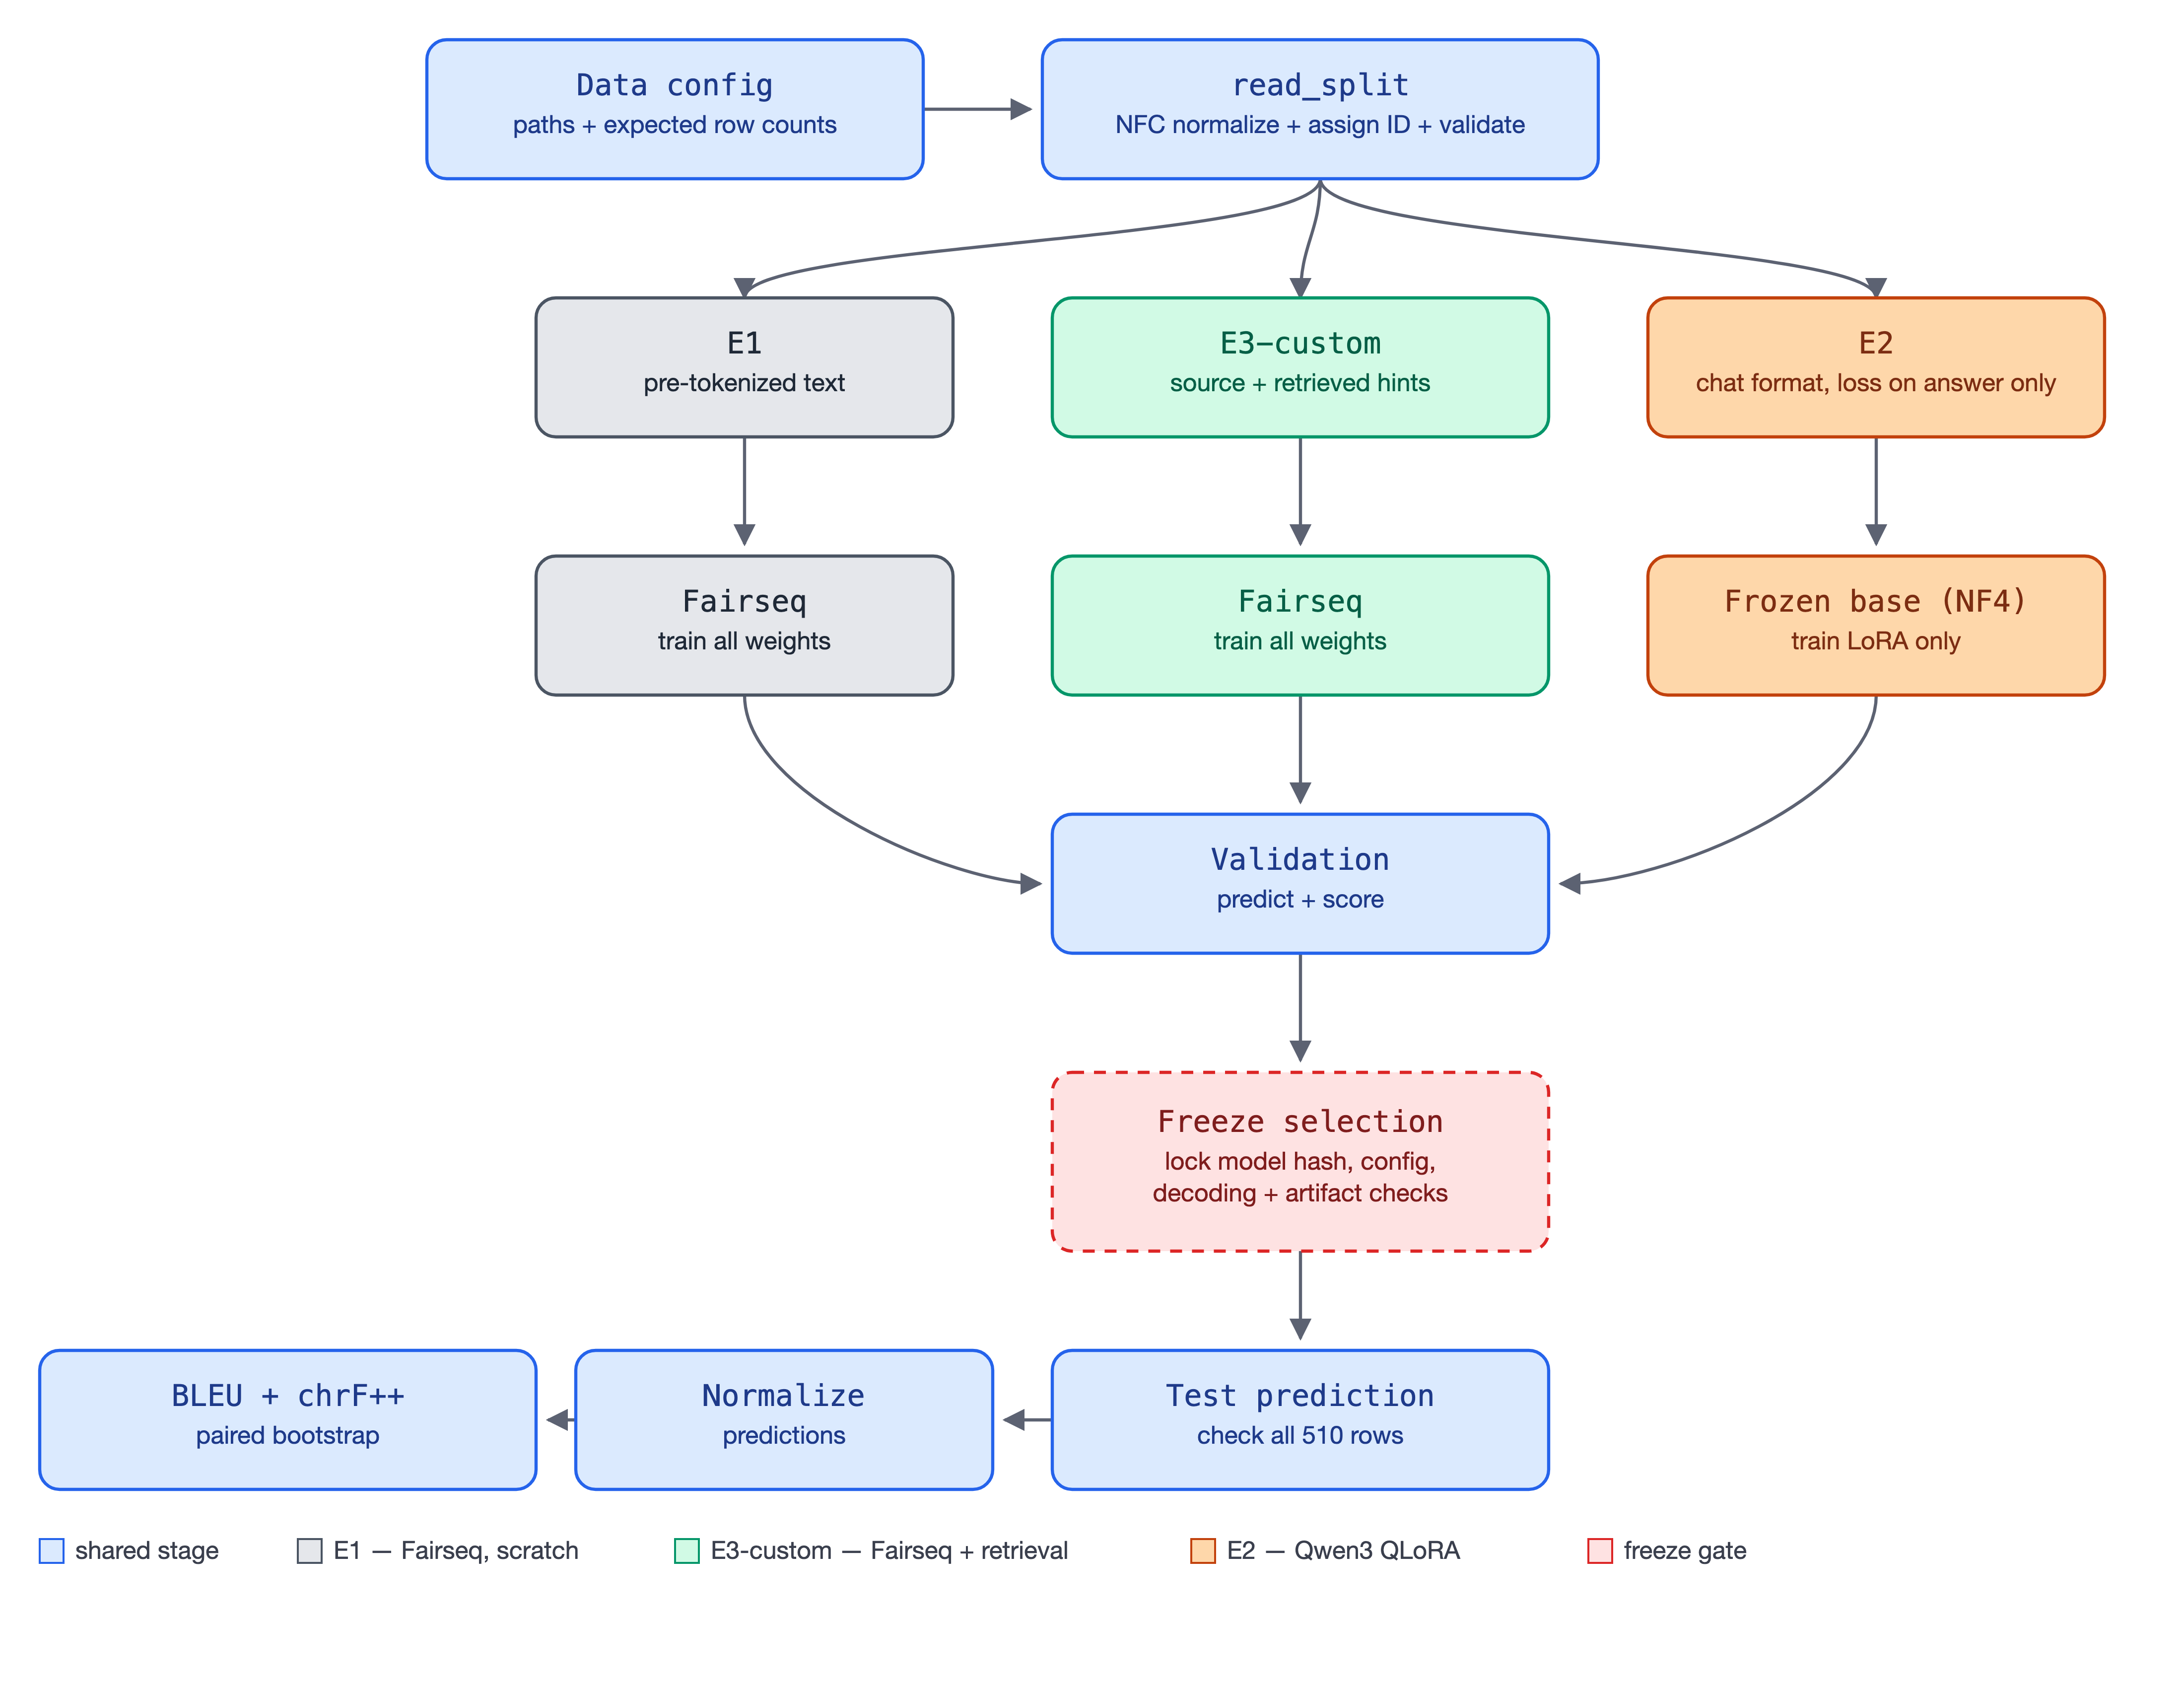
\includegraphics[width=\linewidth]{img/mt_pipeline.png}
%     \caption{Tổng quan pipeline}
%     \label{fig:pipeline}
%   \end{figure}
% \subsection{Thí nghiệm 1 (E1): Transformer huấn luyện từ đầu}
% \subsubsection{Về kiến trúc Transformer và ảnh hưởng của nó lên các bài dịch máy}
% \subsubsection{Fairseq}
% \subsubsection{Hàm mục tiêu}
% \subsubsection{Decode}
% \texttt{E1} sử dụng kiến trúc Transformer encoder--decoder tiêu
% chuẩn~\cite{vaswani2017attention}, triển khai bằng
% Fairseq~\cite{ott2019fairseq} toolkit của Meta. 

% Fairseq là một thư viện mã nguồn mở được xây dựng trên PyTorch để phát triển
% các mô hình xử lý chuỗi, đặc biệt cho dịch máy, tóm tắt văn bản và mô hình ngôn
% ngữ~\cite{ott2019fairseq}. Thư viện cung cấp một quy trình thống nhất gồm xây
% dựng dictionary, chuyển corpus sang định dạng nhị phân, huấn luyện mô hình,
% quản lý checkpoint và sinh chuỗi bằng các thuật toán như beam search. Fairseq
% cũng hỗ trợ batch theo số lượng token, huấn luyện hỗn hợp độ chính xác và tích
% lũy gradient, nhờ đó có thể huấn luyện mô hình dịch máy trong điều kiện bộ nhớ
% GPU giới hạn.


% Trên nền của framework này, E1 sử dụng kiến trúc Transformer bao gồm các thành phần chính như Encoder và decoder cùng có sáu lớp; mỗi lớp
% dùng biểu diễn 512 chiều, tầng feed-forward 2.048 chiều, tám attention head và
% dropout 0,1. Embedding đầu vào và ma trận chiếu đầu ra của decoder được chia
% sẻ trọng số. Mô hình có 67.652.608 tham số và toàn bộ tham số đều được tối ưu từ đầu mà không thông qua bất kì các phương pháp fine-tuning nào. Cụ thể hơn, trong thí nghiệm này, Fairseq giúp đảm nhận việc xây dựng từ điển chỉ từ tập train, chuyển các cặp câu đã được tokenize sang định dạng nhị phân, hỗ trợ tối ưu tham số mô hình, theo dõi metrics như BLEU trên tập validation, lưu các checkpoint tốt nhất để thực hiện việc inference. Nhưng cũng phải lưu ý thêm là các tham số đang được lựa chọn cho thí nghiệm này không phải là các tham số tốt nhất. 

% Ở phía tiếng Việt, đơn vị đầu vào là token đã có sẵn trong corpus; ở phía Hán
% văn, mỗi ký tự là một token. Fairseq xây dictionary chỉ từ tập train, với
% \texttt{--thresholdsrc} và \texttt{--thresholdtgt} cùng bằng 1 đồng nghĩa với việc mọi token nếu xuất hiện ít nhất 1 lần trong tập train sẽ đều được dưa vào dictionary tương ứng. Vì vậy mà pipeline không loại bỏ token train dựa trên tần suất. Tuy nhiên cũng không thể loại bỏ việc các token chỉ trong trong các tập validation/test cũng sẽ nằm ngoài tập train, dẫn đến chúng sẽ bỉ ánh xạ thành token \texttt{<unk>}.


% Ta xét objective function như sau:  Gọi $x$ là câu nguồn tiếng Việt và
% $y_{1:T}=(y_1,\ldots,y_T)$ là câu đích gồm $T$ token Hán văn. Tại vị trí
% $t$, decoder ước lượng phân phối xác suất
% \[
%   p(v\mid y_{<t},x), \qquad v\in V,
% \]
% trên toàn bộ dictionary đích $V$. Trong đó, $y_{<t}$ là các token đích đứng
% trước vị trí $t$. Trong quá trình huấn luyện, mô hình nhận các token đích đúng
% ở những vị trí trước để dự đoán token tiếp theo; cơ chế này được gọi là
% \emph{teacher forcing}.

% Nếu không sử dụng label smoothing, hàm cross-entropy có dạng
% \begin{equation}
%   \mathcal{L}_{\mathrm{CE}}
%   =
%   -\sum_{t=1}^{T}
%   \log p(y_t\mid y_{<t},x).
%   \label{eq:e1-standard-ce}
% \end{equation}
% Mỗi số hạng là negative log-likelihood của token đúng tại một vị trí. Khi mô
% hình gán xác suất cao cho $y_t$, giá trị $-\log p(y_t\mid y_{<t},x)$ nhỏ;
% ngược lại, nếu xác suất của token đúng thấp thì loss tăng.

% Trong E1, Fairseq áp dụng label smoothing với
% $\varepsilon=0{,}1$. Phân phối mục tiêu tại vị trí $t$ được định nghĩa là
% \begin{equation}
%   q_t(v)
%   =
%   \begin{cases}
%     1-\varepsilon, & \text{nếu } v=y_t,\\[3pt]
%     \displaystyle\frac{\varepsilon}{|V|-1},
%       & \text{nếu } v\neq y_t.
%   \end{cases}
%   \label{eq:e1-smoothed-target}
% \end{equation}
% Thay vì gán toàn bộ xác suất mục tiêu bằng 1 cho token đúng và 0 cho mọi token
% khác, label smoothing dành $1-\varepsilon=0{,}9$ cho token đúng và phân phối
% phần xác suất còn lại cho các token khác trong dictionary.

% Hàm mất mát được sử dụng là cross-entropy giữa phân phối mục tiêu đã làm trơn
% $q_t$ và phân phối dự đoán $p$:
% \begin{equation}
%   \mathcal{L}_{\mathrm{E1}}
%   =
%   -\sum_{t=1}^{T}\sum_{v\in V}
%   q_t(v)\log p(v\mid y_{<t},x).
%   \label{eq:e1-loss}
% \end{equation}
% Tương đương,
% \begin{equation}
%   \mathcal{L}_{\mathrm{E1}}
%   =
%   -\sum_{t=1}^{T}
%   \left[
%     (1-\varepsilon)\log p(y_t\mid y_{<t},x)
%     +
%     \frac{\varepsilon}{|V|-1}
%     \sum_{\substack{v\in V\\v\neq y_t}}
%     \log p(v\mid y_{<t},x)
%   \right].
%   \label{eq:e1-loss-expanded}
% \end{equation}
% Các vị trí padding không đóng góp vào loss vì Fairseq loại chúng bằng
% \texttt{ignore\_index}.

% \begin{table}[tbp]
%   \centering
%   \small
%   \renewcommand{\arraystretch}{1.15}
%   \caption{Ký hiệu trong hàm mất mát của E1.}
%   \label{tab:e1-loss-notation}
%   \begin{tabularx}{\textwidth}{@{}p{2.2cm}X@{}}
%     \toprule
%     \textbf{Ký hiệu} & \textbf{Ý nghĩa} \\
%     \midrule
%     $x$
%       & Câu nguồn tiếng Việt. \\

%     $y_{1:T}$
%       & Toàn bộ câu đích Hán văn gồm $T$ token. Trong E1, mỗi token đích
%         tương ứng với một ký tự. \\

%     $y_t$
%       & Ký tự đích đúng tại vị trí $t$. \\

%     $y_{<t}$
%       & Các ký tự đích đứng trước vị trí $t$, tức
%         $(y_1,\ldots,y_{t-1})$. \\

%     $V$
%       & Dictionary đích được xây từ tập train; $|V|$ là số mục trong
%         dictionary. Với E1, $|V|=5.392$, bao gồm các ký hiệu đặc biệt của
%         Fairseq. \\

%     $v$
%       & Một token bất kỳ trong dictionary đích $V$. \\

%     $p(v\mid y_{<t},x)$
%       & Xác suất mà decoder gán cho token $v$ tại vị trí $t$, sau khi quan sát
%         câu nguồn và các token đích trước đó. \\

%     $q_t(v)$
%       & Xác suất mục tiêu sau khi áp dụng label smoothing. \\

%     $\varepsilon$
%       & Hệ số label smoothing; E1 sử dụng $\varepsilon=0{,}1$. \\

%     $\mathcal{L}_{\mathrm{E1}}$
%       & Tổng loss trên các vị trí đích không phải padding. Đây là đại lượng
%         được tối thiểu hóa trong quá trình huấn luyện. \\
%     \bottomrule
%   \end{tabularx}
% \end{table}



%   \begin{table}[tbp]
%     \centering
%     \small
%     \renewcommand{\arraystretch}{1.15}
%     \setlength{\tabcolsep}{5pt}
%     \caption{Cấu hình huấn luyện và giải mã của mô hình E1.}
%     \label{tab:e1-training-config}
%     \begin{tabularx}{\textwidth}{@{}p{3.2cm}p{3.0cm}X@{}}
%       \toprule
%       \textbf{Thành phần}
%         & \textbf{Giá trị}
%         & \textbf{Diễn giải} \\
%       \midrule

%       \multicolumn{3}{@{}l}{\textit{Tối ưu hóa}} \\[2pt]

%       Bộ tối ưu
%         & Adam
%         & Sử dụng $\beta_1=0{,}9$ và $\beta_2=0{,}998$. \\

%       Learning rate cực đại
%         & $5\times10^{-4}$
%         & Learning rate tăng dần trong giai đoạn warmup, sau đó giảm theo lịch
%           \texttt{inverse\_sqrt}. \\

%       Warmup
%         & 8.000 update
%         & Giảm nguy cơ cập nhật quá mạnh trong giai đoạn đầu của quá trình
%           huấn luyện. \\

%       Weight decay
%         & 0
%         & Không áp dụng regularization dựa trên chuẩn của trọng số. \\

%       Gradient clipping
%         & 0
%         & Không giới hạn chuẩn gradient. \\

%       \addlinespace
%       \multicolumn{3}{@{}l}{\textit{Batch và tài nguyên tính toán}} \\[2pt]

%       Kích thước mini-batch
%         & Tối đa 1.000 token/GPU
%         & Fairseq tạo batch động dựa trên tổng số token thay vì cố định số câu. \\

%       Tích lũy gradient
%         & \texttt{update\_freq}=4
%         & Gradient được tích lũy qua bốn mini-batch trước mỗi lần cập nhật
%           trọng số; ngân sách danh nghĩa tối đa xấp xỉ 4.000 token/update. \\

%       Số GPU
%         & 1
%         & Huấn luyện phân tán không được sử dụng. \\

%       Độ chính xác số
%         & fp16
%         & Giảm mức sử dụng bộ nhớ và tăng tốc tính toán trên GPU. \\

%       Seed
%         & 42
%         & Được cố định để kiểm soát các nguồn ngẫu nhiên trong pipeline. \\

%       \addlinespace
%       \multicolumn{3}{@{}l}{\textit{Điều kiện dừng và lựa chọn mô hình}} \\[2pt]

%       Số update tối đa
%         & 50.000
%         & Huấn luyện dừng khi đạt giới hạn này nếu chưa dừng bởi điều kiện khác. \\

%       Số epoch tối đa
%         & 500
%         & Đặt giới hạn trên cho số lần duyệt qua tập train. \\

%       Early stopping
%         & Patience 20
%         & Dừng nếu BLEU trên validation không cải thiện trong 20 epoch liên tiếp. \\

%       Lựa chọn checkpoint
%         & BLEU validation cao nhất
%         & Chỉ checkpoint tốt nhất theo BLEU validation được giữ để sinh bản dịch. \\

%       \addlinespace
%       \multicolumn{3}{@{}l}{\textit{Decoding}} \\[2pt]

%       Phương pháp
%         & Beam search
%         & Duy trì nhiều giả thuyết dịch đồng thời thay vì chọn tham lam từng token. \\

%       Beam size
%         & 7
%         & Giữ tối đa bảy giả thuyết có điểm cao nhất tại mỗi bước giải mã. \\

%       Length penalty
%         & 1,0
%         & Không ưu tiên bổ sung cho bản dịch dài hoặc ngắn khi chuẩn hóa điểm. \\

%       Giới hạn độ dài
%         & $1{,}2|x|+10$
%         & Số token đích tối đa được xác định từ độ dài câu nguồn $|x|$. \\

%       \bottomrule
%     \end{tabularx}
%   \end{table}

%   Các siêu tham số trong Bảng~\ref{tab:e1-training-config} được xác định trước khi
%   huấn luyện. Do giới hạn về tài nguyên tính toán, nghiên cứu không thực hiện tìm
%   kiếm siêu tham số có hệ thống; vì vậy, cấu hình này được xem là một thiết lập
%   baseline có lập luận, không phải cấu hình đã được chứng minh là tối ưu.
% \subsub
% \subsection{Thí nghiệm 2 (E2): Mô hình ngôn ngữ lớn (Qwen3-8B)}
% \subsubsection{Mô hình ngôn ngữ lớn và cấu trúc của Qwen3-8B}
% \subsubsection{Phương pháp Fine-tuning với QLora}
% \subsubsection{Hà}
% \texttt{E2} xuất phát từ một revision cố định của Qwen3-8B (commit được ghim
% trong file cấu hình)~\cite{qwen3technicalreport}. Thay vì cập nhật tám tỷ tham
% số, trọng số nền được lượng tử hoá NF4 4-bit kèm double quantization, và chỉ
% các adapter LoRA được huấn luyện~\cite{hu2021lora,dettmers2023qlora}. Với một
% phép biến đổi tuyến tính có trọng số đóng băng $W$, adapter học hai ma trận
% hạng thấp:
% \begin{equation}
%   h = Wx + \frac{\alpha}{r}BAx,
%   \qquad r=16,\quad \alpha=32.
%   \label{eq:lora}
% \end{equation}
% LoRA được gắn vào mọi module tuyến tính, với dropout bằng 0 và không học bias.
% Mô hình được chuẩn bị bằng \texttt{prepare\_model\_for\_kbit\_training} kết
% hợp gradient checkpointing; phần tính toán chạy ở fp16. Đây là sự đánh đổi
% trực tiếp giữa chi phí bộ nhớ và năng lực thích nghi: mô hình nền cung cấp
% tri thức đa ngữ mạnh, nhưng không được cập nhật đầy đủ và quá trình huấn luyện
% phụ thuộc vào kernel lượng tử hoá.

% \begin{figure}[tbp]
%   \centering
%   \begin{tikzpicture}[
%       font=\footnotesize,node distance=7mm,
%       block/.style={draw,rounded corners,align=center,minimum height=10mm,
%                     text width=29mm},
%       frozen/.style={block,fill=gray!14},
%       trainable/.style={block,fill=orange!14,draw=orange!65!black},
%       data/.style={block,fill=blue!7,draw=blue!55!black},
%       arr/.style={-{Latex[length=1.8mm]},thick}]
%     \node[data] (prompt) {Token chat\\prompt + câu trả lời};
%     \node[frozen,right=of prompt] (base) {Qwen3-8B\\NF4, $W$ đóng băng};
%     \node[trainable,above right=2mm and 8mm of base] (a) {LoRA $A$\\$d\rightarrow r$};
%     \node[trainable,below right=2mm and 8mm of base] (b) {LoRA $B$\\$r\rightarrow d$};
%     \node[data,right=27mm of base] (sum) {$Wx+\frac{\alpha}{r}BAx$\\logits causal LM};
%     \node[trainable,right=of sum] (loss) {Loss chỉ tính trên\\token assistant};
%     \draw[arr] (prompt)--(base);
%     \draw[arr] (base)--node[above,font=\tiny]{nhánh đóng băng}(sum);
%     \draw[arr,orange!75!black] (base.north)|-(a.west);
%     \draw[arr,orange!75!black] (a)--(b);
%     \draw[arr,orange!75!black] (b.east)-|(sum.south);
%     \draw[arr] (sum)--(loss);
%   \end{tikzpicture}
%   \caption{Luồng tham số của \texttt{E2}. Màu xám là trọng số nền đã lượng tử
%   hoá và đóng băng; màu cam là nhánh LoRA duy nhất nhận gradient.}
%   \label{fig:qlora-path}
% \end{figure}

% \subsubsection{Chat template và loss chỉ tính trên câu trả lời}

% Mỗi cặp câu được render thành một lượt system mô tả nhiệm vụ, một lượt user
% chứa câu nguồn và một lượt assistant chứa Hán văn viết liền. Chế độ thinking
% của Qwen3 được tắt ở cả huấn luyện lẫn suy luận để output không lẫn phần lập
% luận. Pipeline render hai lần: một lần dừng ở đầu lượt assistant để lấy
% prefix, và một lần với câu đích đầy đủ; sau đó kiểm tra rằng chuỗi mã hoá đầy
% đủ thực sự bắt đầu bằng prefix trước khi gán nhãn $-100$ cho toàn bộ phần
% prefix. Nhờ vậy:
% \begin{equation}
%   \mathcal{L}_{\mathrm{E2}}
%   = -\sum_{t:\,m_t=1}\log p(y_t\mid z_{<t}),\qquad
%   m_t = \begin{cases}0,&t\in\text{prompt},\\1,&t\in\text{câu trả lời}.
%   \end{cases}
%   \label{eq:response-loss}
% \end{equation}
% Hàm mục tiêu này giúp mô hình không tiêu tốn gradient để học nhắc lại chỉ dẫn.
% Phép kiểm tra prefix biến rủi ro âm thầm khi chat template thay đổi thành một
% lỗi dừng chương trình rõ ràng.

% \begin{figure}[tbp]
%   \centering
%   \begin{tikzpicture}[
%       font=\footnotesize,
%       seg/.style={draw,minimum height=11mm,align=center,inner sep=2mm},
%       mask/.style={seg,fill=gray!13},
%       learn/.style={seg,fill=orange!14,draw=orange!65!black}]
%     \node[mask,text width=29mm] (sys) {chỉ dẫn system\\nhãn $=-100$};
%     \node[mask,text width=27mm,right=0pt of sys] (usr) {user + câu nguồn\\nhãn $=-100$};
%     \node[mask,text width=18mm,right=0pt of usr] (ast) {prefix\\assistant};
%     \node[learn,text width=28mm,right=0pt of ast] (ans) {token đích\\cross-entropy};
%     \node[below=4mm of usr,align=center,font=\scriptsize] (prefix)
%       {chuỗi mã hoá prefix phải là tiền tố chính xác của chuỗi mã hoá đầy đủ};
%     \draw[-{Latex[length=1.5mm]}] (prefix.west)-|(sys.south);
%     \draw[-{Latex[length=1.5mm]}] (prefix.east)-|(ast.south);
%   \end{tikzpicture}
%   \caption{Cơ chế mask của \texttt{E2}: chỉ vùng màu cam đóng góp vào loss.}
%   \label{fig:response-mask}
% \end{figure}

% Sau khi xáo trộn với seed cố định, các ví dụ hoàn chỉnh được gộp tham lam
% (greedy packing) vào cửa sổ 768 token; không ví dụ nào bị cắt đôi nên ranh
% giới mask vẫn chính xác. 19.218 ví dụ trở thành 2.903 chuỗi đã gộp, trong khi
% ví dụ dài nhất chỉ 481 token, nên việc hạ giới hạn từ 1.024 xuống 768 sau bước
% kiểm tra bộ nhớ không cắt mất câu đích nào. Cách gộp này giảm padding, nhưng
% attention không được đặt lại giữa các ví dụ trong cùng một cửa sổ; nói cách
% khác, các ví dụ trong một cửa sổ không hoàn toàn độc lập ở tầng attention.

% \texttt{E2} dùng \texttt{paged\_adamw\_8bit}, learning rate $2\times10^{-4}$
% theo lịch cosine, tỉ lệ warmup 0,05, weight decay 0,01 và gradient clipping
% 1,0. Batch hiệu dụng là 16 cửa sổ đã gộp; ba epoch tương ứng 546 update.
% Checkpoint được đánh giá và lưu sau mỗi 200 step, và được chọn theo
% \texttt{eval\_loss}. Khi suy luận, mô hình dùng beam 4, không sampling, với
% giới hạn độ dài
% \begin{equation}
%   N_{\max}=\min\left(512,\left\lceil2|x|\right\rceil+32\right).
% \end{equation}
% Việc chọn \texttt{eval\_loss} thay cho BLEU, cũng như các hằng số giới hạn độ
% dài, đều chưa được ablation; chúng được báo cáo như một cấu hình cố định.
% \subsection{Thí nghiệm 3 (E3): Huấn luyện mô hình Transformer từ đầu kết hợp Knowledge Injection}

% \texttt{E3-custom} giữ nguyên các khối \texttt{model}, \texttt{training} và
% \texttt{decoding} của \texttt{E1}. Can thiệp duy nhất nằm ở tầng dữ liệu:
% trước bước binarization, pipeline nối thêm các ký tự Hán ứng viên vào cuối câu
% nguồn tiếng Việt. Cơ sở tri thức \texttt{knowledge.json} chứa 16.000 mục và
% bao phủ 5.013 trong số 5.458 ký tự đích phân biệt của corpus (91,85\%). Độ bao
% phủ chỉ cho biết một ký tự có mặt trong cơ sở tri thức hay không; nó không bảo
% đảm ứng viên đúng sẽ được truy hồi, càng không bảo đảm mô hình biết cách sử
% dụng ứng viên đó.

% Chỉ mục tra cứu được xây dựng bằng cách gom các chuỗi tiếng Việt từ các trường
% \texttt{pronunciation}, \texttt{nom\_query}, \texttt{lookup\_\allowbreak query}
% và \texttt{query\_\allowbreak variants}, sau khi casefold và chuẩn hoá khoảng
% trắng. Với chuỗi token nguồn $x_{1:n}$, bộ truy hồi quét mọi vị trí bắt đầu
% với mọi độ dài của các dạng tra cứu đã biết. Mỗi span khớp làm tăng số đếm
% $m(c,x)$ cho những ký tự $c$ mà dạng đó có thể biểu diễn. Các ứng viên được
% sắp xếp theo khoá:
% \begin{equation}
%   \operatorname{rank}(c\mid x)
%   = \bigl(-m(c,x),\;-f_{\mathrm{train}}(c),\;\operatorname{Unicode}(c)\bigr),
%   \label{eq:retrieval-rank}
% \end{equation}
% trong đó $f_{\mathrm{train}}$ chỉ được tính trên câu đích của tập train. Thành
% phần thứ hai vì thế không đọc dữ liệu validation hay test, còn tiêu chí
% Unicode bảo đảm kết quả xác định khi hai ứng viên có điểm bằng nhau.

% \begin{figure}[tbp]
%   \centering
%   \begin{tikzpicture}[
%       font=\footnotesize,node distance=7mm,
%       box/.style={draw,rounded corners,align=center,text width=28mm,
%                   minimum height=11mm,inner sep=2mm},
%       data/.style={box,fill=green!9,draw=green!45!black},
%       warn/.style={box,fill=red!5,draw=red!55!black},
%       arr/.style={-{Latex[length=1.8mm]},thick}]
%     \node[data] (kb) {Cơ sở tri thức\\6.389 dạng tra cứu};
%     \node[data,right=of kb] (match) {Khớp span\\đếm ứng viên};
%     \node[data,right=of match] (rank) {Xếp hạng: số lần khớp\\tần suất train\\Unicode};
%     \node[data,right=of rank] (append) {Nối sentinel\\+ tối đa $k\leq64$ gợi ý};
%     \node[warn,below=8mm of match] (length) {Câu nguồn dài gấp $\approx4$\\số câu mỗi batch giảm $\approx4$};
%     \node[warn,below=8mm of append] (vocab) {Từ vựng nguồn gấp $4{,}8$\\tham số $+10{,}3\%$};
%     \draw[arr] (kb)--(match); \draw[arr] (match)--(rank); \draw[arr] (rank)--(append);
%     \draw[arr] (append.south)--++(0,-3mm)-|(length.east);
%     \draw[arr] (append)--(vocab);
%   \end{tikzpicture}
%   \caption{Quy trình truy hồi của \texttt{E3-custom} và các hệ quả ngoài ý
%   định: tuy chỉ sửa phía nguồn, can thiệp này vẫn làm thay đổi kích thước mô
%   hình và động lực tối ưu.}
%   \label{fig:knowledge-retrieval}
% \end{figure}

% Khi có ứng viên, câu nguồn được render thành
% \texttt{$x_1\ldots x_n$ \_\_knowledge\_\_ $h_1\ldots h_k$}, với $k\leq64$ và
% tiếp tục bị cắt để không vượt quá 256 vị trí encoder. Con số 64 không kèm
% ablation hay lập luận nào được ghi lại; artifact cho thấy 100\% số dòng đều
% được bổ sung gợi ý, với trung bình 61,5--62,4 ứng viên mỗi câu, tức bộ truy
% hồi gần như luôn chạm trần ở mọi split. Đây là một thiết kế thiên về recall
% cao nhưng gần như không có tính chọn lọc.

% Việc bổ sung gợi ý làm độ dài câu nguồn trong train tăng từ trung bình 20,92
% lên 83,44 token trước EOS. Dictionary phía nguồn tăng từ 3.616 lên 17.264
% type. Do \texttt{E1} chỉ chia sẻ embedding đầu vào và đầu ra của decoder,
% embedding của encoder phải mở rộng thêm $13.648\times512=6.987.776$ tham số;
% tổng số tham số vì vậy tăng từ 67.652.608 lên 74.640.384. Với cùng giới hạn
% 1.000 token mỗi GPU, mỗi batch do đó chứa ít câu hơn hẳn. Nói cách khác,
% \texttt{E1} và \texttt{E3-custom} là phép so sánh giữa hai quy trình dùng chung
% cấu hình khai báo nhưng khác nhau về kích thước mô hình và về số câu thực tế
% trong mỗi batch; không nên xem đây là phép đo cô lập tác động của truy hồi.

% \paragraph{Phân biệt với E3 chính thức.}
% Hệ thống \texttt{e3\_fairseq\_knowledge} trong đặc tả của phòng lab đòi hỏi
% phần tích hợp \texttt{knowledge\_v2}, vốn chưa được cung cấp, nên backend chủ
% động dừng. Hệ thống đã thực sự chạy mang định danh riêng
% \texttt{e3\_custom\_fairseq\_knowledge\_vi\_zh\_v1}; vì vậy mọi bảng biểu và
% diễn giải đều phải giữ hậu tố \emph{custom}. Thí nghiệm \texttt{E4} (Qwen3 kết
% hợp cùng cơ chế truy hồi) mới chỉ được triển khai và kiểm tra tiền chạy, chưa
% được huấn luyện, nên nằm ngoài phạm vi phần này.
% \subsection{Cách đánh giá}
% \subsubsection{Các chỉ số được sử dụng cho mục đích đánh giá}
% \subsubsection{Quy trình đánh giá chính}
% \subsection{Config của 3 thí nghiệm và cách thiết lập trong code}

% Bảng~\ref{tab:configs} so sánh cấu hình được khai báo của ba hệ thống. Cần lưu
% ý rằng batch của Fairseq tính theo token, còn batch của \texttt{E2} tính theo
% cửa sổ đã gộp, nên không thể quy hai đại lượng này về cùng một thang ``số câu
% mỗi update''.

% \begin{table}[tbp]
%   \centering
%   \footnotesize
%   \renewcommand{\arraystretch}{1.16}
%   \setlength{\tabcolsep}{3.5pt}
%   \caption{Cấu hình mô hình, huấn luyện và giải mã của ba hệ thống.}
%   \label{tab:configs}
%   \begin{tabularx}{\textwidth}{@{}>{\bfseries}p{2.45cm}XXX@{}}
%     \toprule
%     Thuộc tính & \texttt{E1} & \texttt{E2} & \texttt{E3-custom} \\
%     \midrule
%     Kiến trúc nền
%       & Transformer 6+6 lớp, $d=512$
%       & Qwen3-8B NF4 + LoRA $r=16$
%       & Như \texttt{E1}, câu nguồn có gợi ý \\
%     Tham số
%       & 67,65M, huấn luyện toàn bộ
%       & 8B đóng băng + LoRA huấn luyện được
%       & 74,64M, huấn luyện toàn bộ \\
%     Dạng câu đích
%       & Tách theo ký tự & Hán văn viết liền & Tách theo ký tự \\
%     Hàm mục tiêu
%       & CE có label smoothing 0,1 & CE causal, chỉ trên câu trả lời & Như \texttt{E1} \\
%     Bộ tối ưu
%       & Adam, $5\times10^{-4}$, inverse-sqrt
%       & Paged AdamW 8-bit, $2\times10^{-4}$, cosine
%       & Như \texttt{E1} \\
%     Batch khai báo
%       & 1.000 token $\times$ tích luỹ 4
%       & 1 cửa sổ $\times$ tích luỹ 16
%       & Như \texttt{E1} \\
%     Chọn checkpoint
%       & BLEU validation, patience 20
%       & Loss validation, mỗi 200 step
%       & BLEU validation, patience 20 \\
%     Giải mã
%       & Beam 7; $1{,}2|x|+10$
%       & Beam 4; $\min(512,\lceil2|x|\rceil+32)$
%       & Như \texttt{E1} \\
%     \bottomrule
%   \end{tabularx}
% \end{table}

% Cấu hình khai báo và quá trình chạy thực tế khác nhau đáng kể
% (Bảng~\ref{tab:realized}). Báo cáo cả hai giúp tránh việc hiểu nhầm các giới
% hạn như \texttt{max\_update} là lượng huấn luyện đã thực sự diễn ra.

% \begin{table}[tbp]
%   \centering
%   \footnotesize
%   \renewcommand{\arraystretch}{1.18}
%   \caption{Cấu hình dừng và chọn mô hình so với hành vi thực tế của các lần
%   chạy đã sinh artifact. Đây là thông tin về phương pháp, không phải kết quả
%   dịch.}
%   \label{tab:realized}
%   \begin{tabularx}{\textwidth}{@{}>{\bfseries}p{2.2cm}XXX@{}}
%     \toprule
%     & \texttt{E1} & \texttt{E2} & \texttt{E3-custom} \\
%     \midrule
%     Giới hạn khai báo
%       & 50k update; 500 epoch; patience 20
%       & 3 epoch, tương đương 546 step
%       & Như \texttt{E1} \\
%     Thực tế
%       & Dừng ở epoch 171, update 24.791
%       & Hoàn tất đủ 546 step
%       & Chạm mốc 50.000 update ở epoch 87 \\
%     Checkpoint được chọn
%       & BLEU tốt nhất ở epoch 151
%       & Loss tốt nhất ở step 400; chỉ có hai điểm đánh giá
%       & BLEU tốt nhất ở epoch 77 \\
%     Batch quan sát được
%       & Trung bình 132,5 câu/update
%       & 16 cửa sổ đã gộp/update
%       & Trung bình 33,3 câu/update \\
%     Lưu ý chính
%       & Checkpoint nối tiếp một lần chạy bị ngắt giữa chừng
%       & Bản ghi đóng băng không khớp byte với cấu hình hiện tại
%       & Không cân bằng ngân sách huấn luyện với \texttt{E1} \\
%     \bottomrule
%   \end{tabularx}
% \end{table}

% Ba lưu ý ở hàng cuối không làm thay đổi prediction hay metric đã lưu, nhưng
% chúng giới hạn những phát biểu có thể đưa ra về khả năng tái lập và về quan hệ
% nhân quả. Với \texttt{E1}, checkpoint là kiểm chứng được, song không thể tái
% tạo bằng một lệnh chạy sạch duy nhất vì quá trình huấn luyện đã được nối tiếp
% từ epoch 5, update 579. Với \texttt{E2}, cấu hình huấn luyện và khối giải mã
% vẫn còn trong manifest và trong các dòng prediction, nhưng không thể chứng
% minh từ bản ghi đóng băng hiện tại rằng trạng thái của \texttt{prompt} và
% \texttt{model.*} tại đúng thời điểm sinh kết quả trên test là như đã ghi.
% Những chi tiết này cần được nhắc lại ở phần Hạn chế, thay vì bị che lấp bởi
% một tuyên bố chung chung về khả năng tái lập.

% \subsection{Chọn mô hình trên validation và thực hiện test}

% Mỗi hệ thống lần lượt được huấn luyện, dự đoán và chấm điểm trên validation,
% sau đó lựa chọn được đóng băng, rồi mới dự đoán trên test. Bước
% \texttt{freeze-selection} ghi lại hash của file cấu hình, của
% checkpoint/adapter, của khối giải mã, của prediction trên validation và của
% metric trên validation. Trước mỗi lần giải mã test, hàm
% \texttt{ensure\_selection\_frozen} tính lại toàn bộ các giá trị này. Mọi thay
% đổi hậu nghiệm đối với mô hình hay tham số beam sẽ khiến pipeline dừng lại,
% thay vì sinh ra một điểm test mới.

% \begin{figure}[tbp]
%   \centering
%   \begin{tikzpicture}[
%       font=\footnotesize,node distance=7mm,
%       flowstep/.style={draw,rounded corners,align=center,minimum height=9mm,
%                        text width=28mm,fill=blue!7},
%       gate/.style={draw,diamond,aspect=2.2,align=center,inner sep=1.5mm,
%                    fill=red!5,draw=red!55!black},
%       arr/.style={-{Latex[length=1.8mm]},thick}]
%     \node[flowstep] (train) {Huấn luyện};
%     \node[flowstep,right=of train] (valp) {Dự đoán + chấm\\validation};
%     \node[flowstep,right=of valp] (select) {Chọn\\checkpoint};
%     \node[gate,below=8mm of select] (freeze) {hash\\khớp?};
%     \node[flowstep,below left=9mm and 8mm of freeze] (test) {Dự đoán\\test};
%     \node[flowstep,below=of test] (metric) {Chuẩn hoá + chấm\\+ bootstrap};
%     \node[below right=9mm and 8mm of freeze,align=center,text width=38mm] (stop)
%       {Dừng nếu cấu hình, checkpoint, khối giải mã hoặc artifact validation
%        thay đổi};
%     \draw[arr] (train)--(valp); \draw[arr] (valp)--(select);
%     \draw[arr] (select)--(freeze);
%     \draw[arr] (freeze.south west)--node[left,font=\scriptsize]{có}(test.north);
%     \draw[arr] (test)--(metric);
%     \draw[-{Latex[length=1.8mm]},thick,red!65!black]
%       (freeze.south east)--node[right,font=\scriptsize]{không}(stop.north);
%   \end{tikzpicture}
%   \caption{Cổng validation--test: cam kết không tinh chỉnh trên tập test được
%   cơ học hoá thành một điều kiện kiểm tra bằng hash.}
%   \label{fig:freeze-gate}
% \end{figure}

% Cổng kiểm soát này bảo vệ \emph{quy trình}, chứ không làm cho tiêu chí chọn
% checkpoint trở nên giống nhau giữa các hệ thống. \texttt{E1} và
% \texttt{E3-custom} dùng BLEU nội bộ của Fairseq, còn \texttt{E2} dùng loss và
% chỉ có hai điểm đánh giá. Vì vậy, phép so sánh cuối cùng phản ánh cả chiến
% lược chọn checkpoint. Không có thay đổi hậu nghiệm nào được thực hiện để làm
% các tiêu chí này đồng nhất sau khi kết quả test đã được sinh ra.

% \subsection{Chấm điểm và so sánh các phương pháp}

% \subsubsection{Metric cấp ký tự trên dạng chuẩn}

% Mỗi file prediction dạng JSONL phải có đúng 510 dòng theo cùng thứ tự ID,
% không trùng ID và chỉ chứa một cặp thí nghiệm--split. Trước khi chấm, bộ đánh
% giá tự tính lại
% \texttt{score\_form\_\allowbreak chinese(prediction)} và từ chối file nếu giá
% trị này khác với trường \texttt{prediction\_scored}. Phép kiểm tra này ngăn
% những output đã bị chỉnh tay hoặc được chuẩn hoá bằng đoạn code khác lọt vào
% bước tính metric.

% BLEU được tính bằng SacreBLEU~\cite{papineni2002bleu,post2018sacrebleu}, còn
% chrF++ theo Popovi\'c~\cite{popovic2017chrfpp}; cấu hình chi tiết nằm trong
% Bảng~\ref{tab:metrics}. Vì các bước phía trước đã chèn khoảng trắng giữa mọi
% codepoint, tokenizer \texttt{13a} gần như không còn đơn vị từ nào để phân
% tách: BLEU được báo cáo ở đây thực chất là BLEU cấp ký tự. Tương tự, với
% \texttt{whitespace=false}, thành phần word bigram của chrF++ cũng vận hành
% trên các đơn vị đã được tách sẵn, tức là trên ký tự. Các điểm số này so sánh
% hợp lệ giữa ba hệ thống trong nghiên cứu, nhưng không cùng thang đo với BLEU
% cấp từ trên câu đích tiếng Anh hay tiếng Việt.

% \begin{table}[tbp]
%   \centering
%   \small
%   \renewcommand{\arraystretch}{1.18}
%   \caption{Cấu hình đánh giá được lưu trong mọi artifact metric.}
%   \label{tab:metrics}
%   \begin{tabularx}{\textwidth}{@{}>{\bfseries}p{2.5cm}p{4.7cm}X@{}}
%     \toprule
%     Thành phần & Thiết lập & Ý nghĩa \\
%     \midrule
%     SacreBLEU
%       & v2.6.0; phân biệt hoa thường; tokenizer 13a; exponential smoothing;
%         tắt effective order
%       & BLEU corpus với n-gram 1--4 trên chuỗi đã tách theo ký tự \\
%     chrF2++
%       & v2.6.0; $n_c=6$; $n_w=2$; $\beta=2$; tắt whitespace
%       & F-score ưu tiên recall, kết hợp n-gram ký tự và n-gram \emph{từ} \\
%     Đơn vị đánh giá
%       & 510 \texttt{sample\_id} ghép cặp, mỗi mẫu một câu tham chiếu
%       & Giữ độ khó của câu đồng nhất trong mọi phép so sánh giữa các hệ thống \\
%     Bootstrap
%       & 1.000 lần lấy mẫu lại, seed 42, khoảng percentile 2,5--97,5
%       & Ước lượng độ bất định của chênh lệch metric ở cấp corpus \\
%     \bottomrule
%   \end{tabularx}
% \end{table}

% \subsubsection{Paired bootstrap}
%   Để kiểm tra liệu chênh lệch giữa hai hệ thống có ổn định trên các câu test hay
%   chỉ xuất phát từ một số câu cụ thể, nhóm sử dụng phương pháp paired bootstrap
%   resampling~\cite{koehn2004statistical}. Hai hệ thống $A$ và $B$ được đánh giá
%   trên cùng $N=510$ câu và có cùng câu tham chiếu. Trong mỗi lần lặp bootstrap,
%   $N$ vị trí được lấy mẫu có hoàn lại từ tập test. Cùng một tập vị trí được dùng
%   để tính lại metric cho cả hai hệ thống, nhờ đó phép so sánh vẫn được thực hiện
%   trên đúng các câu giống nhau.

%   Gọi $I_b$ là tập chỉ số được lấy mẫu ở lần lặp thứ $b$, $R$ là tập câu tham
%   chiếu và $M$ là metric BLEU hoặc chrF++. Chênh lệch giữa hệ thống $B$ và hệ
%   thống $A$ trong lần lặp thứ $b$ được tính bởi
%   \begin{equation}
%     \Delta^{(b)}
%     =
%     M\!\left(B_{I_b},R_{I_b}\right)
%     -
%     M\!\left(A_{I_b},R_{I_b}\right),
%     \qquad b=1,\ldots,1000.
%   \end{equation}
%   Trong đó, $\Delta^{(b)}>0$ cho biết hệ thống $B$ đạt điểm cao hơn $A$ trên mẫu
%   bootstrap tương ứng.

%   Từ 1.000 giá trị $\Delta^{(b)}$, khoảng tin cậy bootstrap 95\% được xác định
%   bằng các percentile 2,5\% và 97,5\%. Nếu khoảng này chứa 0, dữ liệu chưa cung
%   cấp đủ bằng chứng rằng hai hệ thống khác nhau một cách ổn định. Ngược lại, nếu
%   toàn bộ khoảng nằm về một phía của 0, chênh lệch quan sát được nhất quán hơn
%   trên các mẫu bootstrap.

%   P-value hai phía được ước lượng từ tỷ lệ các giá trị $\Delta^{(b)}$ nằm ở mỗi
%   phía của 0. Pipeline lấy tỷ lệ ở phía có ít mẫu hơn, nhân đôi và áp dụng hiệu
%   chỉnh $+1$ cho cả tử số và mẫu số để tránh p-value bằng 0 khi chỉ sử dụng một
%   số hữu hạn lần lặp. Tất cả phép so sánh sử dụng 1.000 lần lấy mẫu và seed 42.

%   Việc lấy mẫu theo cặp giúp tập trung phép kiểm định vào chênh lệch dự đoán của
%   hai hệ thống trên cùng các câu test. Tuy nhiên, phép kiểm định này không loại
%   bỏ những yếu tố gây nhiễu khác, chẳng hạn khác biệt về số tham số, dữ liệu đầu
%   vào, quá trình huấn luyện hoặc cách lựa chọn checkpoint.

% \subsection{Các quyết định thiết kế và giới hạn}

% Không phải mọi lựa chọn trong pipeline đều đã được kiểm chứng bằng thí nghiệm
% đối chứng. Vì vậy, Bảng~\ref{tab:decisions} tổng hợp các quyết định thiết kế
% chính, những phương án khác có thể được sử dụng và các giới hạn đi kèm. Mức độ
% căn cứ được chia thành ba nhóm. \emph{Tài liệu} cho biết lý do đã được ghi rõ
% trong đặc tả hoặc tài liệu dự án. \emph{Triển khai} cho biết quyết định được thể
% hiện trong code hoặc artifact, còn lý do được suy ra từ cách triển khai.
% \emph{Chưa đối chứng} cho biết chưa có thí nghiệm chỉ thay đổi riêng yếu tố đó
% để so sánh các phương án.

% \begin{table}[tbp]
%   \centering
%   \scriptsize
%   \renewcommand{\arraystretch}{1.18}
%   \setlength{\tabcolsep}{3pt}
%   \caption{Các quyết định thiết kế, phương án thay thế và giới hạn tương ứng.}
%   \label{tab:decisions}
%   \begin{tabularx}{\textwidth}{@{}p{2.35cm}p{2.05cm}XXp{1.7cm}@{}}
%     \toprule
%     \textbf{Quyết định}
%       & \textbf{Phương án khác}
%       & \textbf{Lý do lựa chọn}
%       & \textbf{Đánh đổi và giới hạn}
%       & \textbf{Căn cứ} \\
%     \midrule

%     Không dùng BPE; giữ ngưỡng tần suất bằng 1
%       & Áp dụng BPE hoặc loại token hiếm
%       & Câu đích đã được tách tới cấp ký tự; mọi token xuất hiện trong train
%         đều được giữ lại
%       & Vẫn không sinh được token chỉ xuất hiện trong validation hoặc test;
%         chưa so sánh trực tiếp với BPE
%       & Tài liệu \\

%     Giữ các cặp trùng lặp và ký tự U+FFFD
%       & Loại cặp trùng; sửa hoặc loại dòng lỗi
%       & Bảo toàn corpus được cung cấp và không tự phỏng đoán ký tự đã mất
%       & Cặp trùng làm một số mẫu có trọng số lớn hơn; 44 câu nguồn được ghép
%         với nhiều câu đích
%       & Tài liệu \\

%     Dùng câu đích viết liền cho \texttt{E2}
%       & Chèn khoảng trắng giữa các Hán tự
%       & Duy trì dạng văn bản tự nhiên phù hợp với đầu vào mà mô hình tiền
%         huấn luyện thường tiếp nhận
%       & Đầu ra phải được chuyển về dạng cấp ký tự trước khi chấm điểm
%       & Triển khai \\

%     Chỉ tính loss trên câu trả lời
%       & Tính loss trên cả prompt và câu trả lời
%       & Tập trung cập nhật vào phần bản dịch mà mô hình cần sinh
%       & Phụ thuộc vào việc xác định đúng ranh giới giữa prompt và câu trả lời;
%         pipeline có kiểm tra ranh giới này
%       & Triển khai \\

%     Ghép nhiều mẫu vào một cửa sổ huấn luyện của \texttt{E2}
%       & Mỗi cửa sổ chỉ chứa một mẫu
%       & Giảm lượng padding và sử dụng bộ nhớ GPU hiệu quả hơn
%       & Attention không được đặt lại giữa các mẫu nằm trong cùng một cửa sổ
%       & Triển khai \\

%     Giới hạn tối đa 64 ký tự gợi ý trong \texttt{E3-custom}
%       & Dùng ít gợi ý hơn hoặc xây dựng bộ xếp hạng chọn lọc hơn
%       & Chưa tìm thấy tài liệu ghi rõ lý do chọn ngân sách 64
%       & Phần lớn câu gần chạm giới hạn; chiều dài nguồn tăng khoảng 3,9 lần
%       & Chưa đối chứng \\

%     Xếp hạng gợi ý bằng tần suất trong train
%       & Dùng bộ xếp hạng có xét ngữ cảnh, chỉ học từ train
%       & Cho kết quả xác định và không sử dụng câu đích của validation hoặc test
%       & Tần suất toàn corpus không cho biết ký tự nào phù hợp nhất với ngữ
%         cảnh cụ thể
%       & Triển khai \\

%     Chọn adapter \texttt{E2} theo validation loss
%       & Chọn theo BLEU validation
%       & Trainer lưu và nạp lại checkpoint có validation loss thấp nhất
%       & Khác tiêu chí chọn mô hình của \texttt{E1} và \texttt{E3-custom};
%         run chỉ có hai thời điểm đánh giá
%       & Chưa đối chứng \\

%     Chấm điểm trên biểu diễn cấp ký tự
%       & Chấm trực tiếp đầu ra theo tokenization riêng của từng hệ thống
%       & Đưa đầu ra của Fairseq và Qwen về cùng một biểu diễn trước khi so sánh
%       & Điểm BLEU thu được không thể so sánh trực tiếp với BLEU cấp từ
%       & Tài liệu \\

%     Khóa lựa chọn mô hình trước khi chạy test
%       & Chỉ kiểm soát bằng quy ước thủ công
%       & Ngăn việc thay đổi checkpoint hoặc cấu hình decoding sau khi đã xem
%         kết quả test
%       & Yêu cầu hash của config, checkpoint và cấu hình decoding phải nhất
%         quán; chuỗi xác minh hiện tại của \texttt{E2} không còn khớp hoàn toàn
%       & Tài liệu \\

%     \bottomrule
%   \end{tabularx}
% \end{table}

% Phép so sánh giữa ba hệ thống dựa trên ba nguyên tắc chính. Thứ nhất, cả ba hệ
% thống xuất phát từ cùng các split dữ liệu, mặc dù cách biểu diễn đầu vào và
% phương pháp huấn luyện khác nhau. Thứ hai, chúng được đánh giá trên cùng 510 câu
% test và cùng các câu tham chiếu. Thứ ba, mọi bản dịch đều được chuyển về cùng
% một biểu diễn cấp ký tự trước khi tính metric. Về mặt thiết kế, pipeline cũng
% yêu cầu lựa chọn checkpoint phải được khóa trước khi sinh dự đoán test; tuy
% nhiên, chuỗi xác minh artifact của \texttt{E2} hiện không còn khớp hoàn toàn
% với config trên đĩa.

% Những biện pháp trên cho phép so sánh chất lượng tổng thể của các hệ thống đã
% triển khai. Tuy nhiên, chúng không đủ để quy toàn bộ chênh lệch điểm số cho một
% thành phần riêng lẻ. Chẳng hạn, không thể kết luận mức thay đổi giữa
% \texttt{E1} và \texttt{E3-custom} chỉ do knowledge retrieval, vì hai hệ thống
% còn khác nhau về chiều dài đầu vào, kích thước từ vựng, số tham số và quá trình
% huấn luyện thực tế. Để xác định tác động riêng của từng lựa chọn, cần thực hiện
% các thí nghiệm đối chứng trong đó chỉ một yếu tố được thay đổi tại mỗi lần so
% sánh.

%\newpage
\section{Thiết lập thực nghiệm}

Chương này trình bày điều kiện triển khai và phạm vi đánh giá của ba hệ thống
E1, E2 và E3-custom. Kiến trúc mô hình, quy trình huấn luyện, tiêu chí lựa chọn
checkpoint, chuẩn hoá đầu ra và phương pháp chấm điểm đã được trình bày trong
phần Phương pháp. Vì vậy, phần này chỉ mô tả phần cứng, môi trường phần mềm,
thiết lập ngẫu nhiên, các ràng buộc tài nguyên và cấu hình triển khai cần thiết
để diễn giải kết quả.

\subsection{Môi trường tính toán}

\subsubsection{Phần cứng}

Ba hệ thống được huấn luyện trên cùng một máy \texttt{laboratory}, sử dụng một
GPU \texttt{NVIDIA GeForce RTX 3060} với 12.488.343.552 byte bộ nhớ (xấp xỉ
12,5~GB). Các run manifest đều ghi nhận
\texttt{distributed\_world\_size=1}; do đó, không kết quả nào trong báo cáo
được tạo bởi thiết lập đa GPU.

E1 và E3-custom được chạy trên
\texttt{Linux-7.0.0-28-generic-x86\_64-with-glibc2.39}. Đoạn chạy tiếp hiện được
ghi trong manifest của E2 sử dụng
\texttt{Linux-7.0.0-30-generic-x86\_64-with-glibc2.39}. Sự khác biệt này phản
ánh trạng thái hệ thống tại thời điểm chạy, không phải khác biệt về phần cứng.
Các notebook Kaggle trong repo chỉ cung cấp đường chạy dự phòng và không sinh
ra các kết quả được báo cáo.

\subsubsection{Môi trường phần mềm}

Dự án duy trì ba môi trường Conda tách biệt để cô lập các phụ thuộc của
Fairseq, QLoRA và bộ đánh giá. Cách tổ chức này tránh việc ép Fairseq 0.12.2 và
các kernel lượng tử hoá 4-bit của \texttt{bitsandbytes} vào cùng một software
stack. Bảng~\ref{tab:compute-env} ghi phiên bản thực tế trong các artifact hiện
có; hàng E2 tương ứng với đoạn chạy tiếp đến step 910.

\begin{table}[tbp]
  \centering
  \small
  \renewcommand{\arraystretch}{1.18}
  \caption{Các môi trường Conda và phiên bản được ghi trong artifact hiện tại.}
  \label{tab:compute-env}
  \begin{tabularx}{\textwidth}{@{}>{\ttfamily}p{2.3cm}p{2.3cm}p{3.15cm}X@{}}
    \toprule
    \normalfont\textbf{Môi trường} & \textbf{Dùng cho}
      & \textbf{Python / PyTorch / CUDA} & \textbf{Thư viện chính} \\
    \midrule
    .conda/\allowbreak fairseq
      & E1, E3-custom
      & 3.10.20 / 1.13.1 / 11.7
      & \texttt{fairseq} 0.12.2 \\
    .conda/llm
      & E2
      & 3.10.20 / 2.6.0+cu124 / 12.4
      & \texttt{transformers} 4.57.6; \texttt{peft} 0.20.0;
        \texttt{bitsandbytes} 0.50.1; \texttt{accelerate} 1.14.0;
        \texttt{datasets} 4.8.5 \\
    .conda/eval
      & Chấm điểm, kiểm toán, kiểm thử
      & 3.10.20 / --- / ---
      & \texttt{sacrebleu} 2.6.0; \texttt{PyYAML} 6.0.2;
        \texttt{pytest} 8.4.1 \\
    \bottomrule
  \end{tabularx}
\end{table}

Tệp khai báo môi trường E2 từng đặt PyTorch 2.5.1, trong khi manifest của đoạn
chạy tiếp ghi \texttt{2.6.0+cu124}; Bảng~\ref{tab:compute-env} ưu tiên phiên bản
đã được ghi nhận khi chạy. Việc chấm điểm được tách khỏi các môi trường huấn
luyện: mọi metric artifact dùng SacreBLEU 2.6.0 và lưu chữ ký chứa
\texttt{version:2.6.0}. Vì vậy, cả ba hệ thống được chấm bằng cùng một phiên bản
bộ đánh giá, dù software stack dùng để huấn luyện khác nhau.

\subsubsection{Kiểm soát ngẫu nhiên và khả năng lặp lại}

Cả ba cấu hình đặt \texttt{seed: 42}. Với Fairseq, pipeline:
\begin{itemize}
  \item bật \texttt{cudnn.deterministic} và tắt
  \texttt{cudnn.benchmark};
  \item gọi \texttt{use\_deterministic\_algorithms} ở chế độ
  \texttt{warn\_only};
  \item đặt \texttt{CUBLAS\_WORKSPACE\_CONFIG=:4096:8} và
  \texttt{PYTHONHASHSEED} cho tiến trình huấn luyện.
\end{itemize}
Với QLoRA, \texttt{set\_seed} được gọi trước khi huấn luyện và sinh dự đoán;
\texttt{TrainingArguments} nhận cả \texttt{seed} và \texttt{data\_seed}; bước
packing sử dụng một generator riêng cũng được khởi tạo từ 42.

Các thiết lập trên làm giảm biến thiên và tăng khả năng lặp lại khi giữ nguyên
ngăn xếp phần cứng và phần mềm. Tuy nhiên, chế độ \texttt{warn\_only} không buộc mọi
CUDA operation phải tất định, nên chúng không cấu thành cam kết tái lập
bit-for-bit khi đổi GPU, driver, CUDA hoặc phiên bản thư viện.

\subsection{Cấu hình triển khai}

\subsubsection{Ràng buộc tài nguyên}

Giới hạn 12,5~GB VRAM chi phối một số lựa chọn triển khai. Với E2, trọng số nền
Qwen3-8B được lượng tử hoá NF4 kèm double quantization; chỉ LoRA adapter nhận
gradient. Cấu hình đồng thời sử dụng gradient checkpointing,
\texttt{paged\_adamw\_8bit}, một packed window trên mỗi thiết bị, tích luỹ
gradient qua 16 bước và độ dài cửa sổ 768 token. Với E1 và E3-custom,
\texttt{max\_tokens\_per\_gpu=1000} kết hợp \texttt{update\_freq=4}, tương ứng
với ngân sách khai báo khoảng 4.000 token cho mỗi lần cập nhật tham số.

Các lựa chọn này mô tả cách ba hệ thống được triển khai trên phần cứng sẵn có;
chúng không phải kết quả của một nghiên cứu ablation về bộ nhớ hoặc batch size.
Ảnh hưởng quan sát được của giới hạn này được trình bày cùng các phát hiện thực
nghiệm.

\subsubsection{Tóm tắt cấu hình thực tế}

Bảng~\ref{tab:exp-recap} cung cấp một bản tóm tắt để đối chiếu nhanh; định nghĩa
đầy đủ của từng mô hình và realized protocol nằm trong phần Phương pháp.

\begin{table}[tbp]
  \centering
  \footnotesize
  \renewcommand{\arraystretch}{1.16}
  \setlength{\tabcolsep}{3.5pt}
  \caption{Tóm tắt cấu hình triển khai của ba hệ thống được đánh giá.}
  \label{tab:exp-recap}
  \begin{tabularx}{\textwidth}{@{}>{\bfseries}p{2.35cm}XXX@{}}
    \toprule
    & E1 & E2 & E3-custom \\
    \midrule
    Khung mô hình
      & Transformer 6+6, $d=512$, 67,65M tham số
      & Qwen3-8B đóng băng + LoRA $r=16$, $\alpha=32$
      & Như E1, nguồn được bổ sung gợi ý, 74,64M tham số \\
    Độ chính xác
      & fp16
      & Trọng số nền NF4 4-bit, double quantization; tính toán fp16
      & fp16 \\
    Bộ tối ưu
      & Adam, $5\times10^{-4}$, inverse-sqrt, warmup 8.000
      & Paged AdamW 8-bit, $2\times10^{-4}$, cosine, warmup ratio 0,05
      & Như E1 \\
    Đơn vị batch
      & 1.000 token $\times$ tích luỹ 4
      & 1 packed window $\times$ tích luỹ 16
      & Như E1 \\
    Ngân sách thực tế
      & Dừng ở epoch 171 / update 24.791
      & Chạy tiếp từ 3 epoch / 546 step đến 5 epoch / 910 step
      & Chạm 50.000 update ở epoch 87 \\
    Chọn checkpoint
      & Validation BLEU, epoch 151
      & Validation \texttt{eval\_loss}, step 400
      & Validation BLEU, epoch 77 \\
    Giải mã
      & Beam 7; $1{,}2|x|+10$
      & Beam 4; $\min(512,\lceil2|x|\rceil+32)$
      & Như E1 \\
    \bottomrule
  \end{tabularx}
\end{table}

Đơn vị batch của hai backend không quy đổi trực tiếp: Fairseq giới hạn số token
trên mỗi GPU, còn E2 đếm các cửa sổ đã packing. Do đó, hàng “Đơn vị batch”
không được diễn giải như một so sánh về số câu trong mỗi update.

\subsection{Phạm vi thực nghiệm}

Báo cáo so sánh ba hệ thống dịch Việt $\rightarrow$ Hán văn trên cùng các phân
hoạch cố định của ngữ liệu \emph{Đại Việt sử ký toàn thư}: E1 là Transformer
huấn luyện từ đầu; E2 là Qwen3-8B thích nghi bằng QLoRA; E3-custom là E1 với
câu nguồn được bổ sung gợi ý Hán tự từ kho tri thức. Đây là so sánh cấp hệ
thống, không phải một chuỗi ablation kiểm soát từng biến. Các bất biến về dữ
liệu, quy trình lựa chọn trên validation, cổng đóng băng tập test và bộ đánh
giá chung đã được định nghĩa trong phần Phương pháp.

Hai hệ thống trong đặc tả ban đầu không thuộc tập kết quả. E3 chính thức phụ
thuộc integration \texttt{knowledge\_v2} chưa có trong repo và vì vậy ở trạng
thái blocked; hệ thống đã chạy phải luôn được ghi là E3-custom. E4, tức Qwen3
kết hợp cơ chế truy hồi của E3-custom, mới được cài đặt và chạy preflight ước
lượng chi phí, chưa được huấn luyện. Báo cáo không gán kết quả định lượng cho
E3 chính thức hoặc E4.


\subsection{Chi phí tính toán và hành vi huấn luyện}

\subsubsection{Chi phí huấn luyện thực đo}

Bảng~\ref{tab:wallclock} tổng hợp thời gian huấn luyện quan sát được trên cùng
một RTX 3060. Các giá trị không bao gồm thời gian tiền xử lý, sinh dự đoán hoặc
chấm điểm.

\begin{table}[tbp]
  \centering
  \small
  \renewcommand{\arraystretch}{1.18}
  \caption{Tổng thời gian huấn luyện ghi nhận của ba hệ thống.}
  \label{tab:wallclock}
  \begin{tabularx}{\textwidth}{@{}>{\bfseries}p{3.4cm}p{3.1cm}X@{}}
    \toprule
    Hệ thống & Tổng wall-clock & Ghi chú \\
    \midrule
    E1
      & $\approx$ 3.209,5 s ($\approx$ 53,5 phút)
      & Cộng khoảng 90 s của lần chạy bị ngắt và 3.119,5 s của đoạn chạy tiếp
        từ checkpoint tại epoch 5 / update 579 \\
    E3-custom
      & 4.758,7 s ($\approx$ 79,3 phút)
      & Một lượt chạy; chạm \texttt{max\_update=50000} \\
    E2
      & 33.940,7 s ($\approx$ 9,43 giờ)
      & Cộng đoạn đầu 20.328,3 s và đoạn chạy tiếp 13.612,4 s từ checkpoint
        546 đến step 910 \\
    \bottomrule
  \end{tabularx}
\end{table}

Tổng của E1 là tổng thời gian còn quan sát được qua hai đoạn, không phải phép đo
của một lượt huấn luyện sạch từ đầu đến cuối. Tương tự, tổng E2 được tái dựng
từ thời gian đã ghi cho đoạn đầu và \texttt{train\_runtime} của đoạn chạy tiếp;
log chi tiết của đoạn đầu không còn trong artifact hiện tại. Vì vậy, các con số
này phù hợp để mô tả chi phí đã ghi nhận, nhưng không nên được diễn giải như
benchmark tốc độ chuẩn hoá giữa các kiến trúc.

\subsubsection{Ảnh hưởng quan sát được của giới hạn bộ nhớ}

Khi E3-custom bổ sung danh sách gợi ý Hán tự, số token nguồn tăng xấp xỉ
3,9 lần. Dưới cùng giới hạn \texttt{max\_tokens\_per\_gpu=1000}, số câu trung
bình trong mỗi update giảm từ 132,5 ở E1 xuống 33,3 ở E3-custom. Vì vậy, E1 và
E3-custom không chỉ khác nhau ở nội dung đầu vào: số câu đóng góp vào mỗi lần
cập nhật cũng khác do giới hạn bộ nhớ. Đây là một confound của phép so sánh cấp
hệ thống, không phải bằng chứng riêng về hiệu quả của cơ chế truy hồi.

\subsubsection{Diễn biến validation và lựa chọn checkpoint của E2}
\label{sec:e2-budget}

E2 ban đầu được huấn luyện trong 3 epoch, tương ứng 546 optimizer step, rồi chạy
tiếp đến 5 epoch và 910 step từ checkpoint 546. Với
\texttt{eval\_steps=200}, toàn bộ quá trình chỉ có bốn điểm đánh giá validation
(Bảng~\ref{tab:e2-budget}).

\begin{table}[tbp]
  \centering
  \small
  \renewcommand{\arraystretch}{1.18}
  \caption{Các điểm đánh giá validation của E2 qua 910 step.}
  \label{tab:e2-budget}
  \begin{tabularx}{\textwidth}{@{}rrrX@{}}
    \toprule
    \textbf{Step} & \textbf{Epoch} & \textbf{\texttt{eval\_loss}}
      & \textbf{Giai đoạn} \\
    \midrule
    200 & 1,10 & 1,4444 & Ba epoch ban đầu \\
    400 & 2,20 & \textbf{1,4322} & Ba epoch ban đầu; checkpoint được chọn \\
    600 & 3,30 & 1,4659 & Đoạn chạy tiếp \\
    800 & 4,40 & 1,5815 & Đoạn chạy tiếp \\
    \bottomrule
  \end{tabularx}
\end{table}

Trong bốn điểm được đo, \texttt{eval\_loss} thấp nhất ở step 400 và cao hơn ở
step 600 và 800. Do Trainer dùng \texttt{load\_best\_model\_at\_end} theo
\texttt{eval\_loss}, adapter xuất ra sau step 910 vẫn mang trọng số của
checkpoint 400. SHA-256 của \texttt{adapter\_model.safetensors} xuất ra trùng
với file tương ứng trong checkpoint 400, trong khi khác checkpoint 800 và 910.

Kết quả này cho thấy phần ngân sách kéo dài không thay đổi checkpoint được chọn;
nó không tạo thành một hệ thống E2 mới. Tuy nhiên, bốn điểm đánh giá là một lưới
thưa và tiêu chí lựa chọn là loss, không phải BLEU. Vì vậy, bằng chứng chỉ hỗ trợ
nhận định rằng validation loss đo được tăng sau step 400; nó không xác định
chính xác thời điểm bắt đầu overfitting và cũng không chứng minh bản dịch ở 5
epoch kém hơn theo BLEU.

% \subsection{Các chỉ số đánh giá} - Phát

% 3. Evaluation Metrics - Phát
% 3.1 SacreBLEU
% 3.2 chrF++
% 3.3 COMET

% \subsection{Evaluation Procedure} - Phát


\subsection{Evaluation Metrics (Chỉ số đánh giá)}

Để đánh giá chất lượng của các mô hình dịch máy từ tiếng Việt sang Hán văn cổ (Việt $\rightarrow$ Hán cổ), nghiên cứu này sử dụng hai chỉ số đánh giá tự động phổ biến: SacreBLEU và chrF++. Do ngữ liệu đích đã được phân tách bằng khoảng trắng ở cấp độ từng Hán tự, các chỉ số này chủ yếu phản ánh mức độ tương đồng ở cấp độ ký tự (character level).

\subsubsection{4.3.1 SacreBLEU}
Chỉ số BLEU (Bilingual Evaluation Understudy) đánh giá độ tương đồng giữa bản dịch do mô hình sinh ra và bản dịch tham chiếu dựa trên tỷ lệ trùng khớp của các n-gram (với $n \le 4$).
\begin{itemize}
    \item \textbf{Cấu hình thực tế:} Điểm BLEU-4 được tính bằng thư viện \texttt{SacreBLEU}, qua đó bảo đảm tính chuẩn hóa và nhất quán. Phiên bản được sử dụng trong kho mã nguồn là \texttt{2.6.0}.
    \item \textbf{Chữ ký cấu hình (signature):} Cấu hình cụ thể của chỉ số BLEU được ghi lại bằng chữ ký tiêu chuẩn \texttt{nrefs:1|case:mixed|eff:no|tok:13a|smooth:exp|version:2.6.0}. Trong đó, phương pháp làm mượt là \texttt{exp} (exponential smoothing) và tùy chọn \texttt{effective\_order} không được sử dụng.
    \item \textbf{Bộ tách từ:} Theo đặc tả, cả bốn nhóm thí nghiệm phải sử dụng thống nhất bộ tách từ Moses để bảo đảm độ tin cậy của phép so sánh giữa các hướng dịch. Trong \texttt{SacreBLEU 2.6.0}, cấu hình \texttt{tok:13a} tương ứng với bộ tách từ \texttt{mteval-v13a} của Moses. Do ngữ liệu Hán văn cổ đích đã được tiền xử lý bằng cách chèn khoảng trắng giữa từng Hán tự, bộ tách từ ít ảnh hưởng đến kết quả; vì vậy, điểm BLEU thu được về cơ bản phản ánh mức độ tương đồng ở cấp độ ký tự.
\end{itemize}

\subsubsection{4.3.2 chrF++}
Chỉ số chrF++ là phiên bản mở rộng của chrF, kết hợp độ tương đồng ở cấp độ ký tự (character-level similarity) với thông tin ở cấp độ từ (word-level information). Chất lượng bản dịch được đánh giá dựa trên độ chính xác (precision), độ bao phủ (recall) và điểm F (F-score).
\begin{itemize}
    \item \textbf{Độ tương đồng ở cấp độ ký tự (character n-gram):} Chỉ số đo tỷ lệ trùng khớp của các n-gram ký tự có độ dài từ 1 đến 6 giữa bản dịch của mô hình và bản dịch tham chiếu. Thành phần này giúp ghi nhận các biến thể về từ vựng và cấu trúc trong Hán văn cổ.
    \item \textbf{Thông tin ở cấp độ từ (word n-gram):} Chỉ số bổ sung tỷ lệ trùng khớp của các n-gram từ có độ dài từ 1 đến 2. Trong ngữ liệu Hán văn cổ đã được phân tách bằng khoảng trắng, mỗi Hán tự được xem như một từ độc lập; do đó, thành phần n-gram từ bậc hai thực chất tương ứng với bigram Hán tự.
    \item \textbf{Precision, recall và F-score:} chrF++ sử dụng hệ số $\beta = 2$ để tính điểm $F_\beta$, tức là đặt trọng số cho recall cao hơn precision. Cách tính này nhấn mạnh khả năng bao phủ các đơn vị nội dung quan trọng trong bản dịch.
    \item \textbf{Chữ ký cấu hình (signature):} Chữ ký của chrF++ trong thực nghiệm là \texttt{nrefs:1|case:mixed|eff:yes|nc:6|nw:2|space:no|version:2.6.0}.
\end{itemize}

\subsubsection{4.3.3 COMET (tùy chọn)}
Chỉ số COMET (Crosslingual Optimized Metric for Evaluation of Translation) sử dụng mô hình ngôn ngữ đa ngữ, chẳng hạn như XLM-RoBERTa, để biểu diễn câu nguồn, bản dịch tham chiếu và bản dịch của mô hình trong một không gian vector chung, từ đó đánh giá chất lượng dịch ở cấp độ câu.
\begin{itemize}
    \item \textbf{Hạn chế khi áp dụng:} Mặc dù COMET thường có độ tương quan cao với đánh giá của con người đối với các ngôn ngữ hiện đại, một số checkpoint chủ yếu được huấn luyện trên dữ liệu thuộc các ngôn ngữ châu Âu. Vì khả năng bao phủ tiếng Việt và đặc biệt là Hán văn cổ có thể còn hạn chế, kết quả đánh giá ngữ nghĩa có nguy cơ thiếu chính xác hoặc kém nhạy. Do đó, COMET chỉ được xem là chỉ số tùy chọn và không được sử dụng làm thước đo chính trong các thực nghiệm của nghiên cứu này.
\end{itemize}

\subsection{Quy trình đánh giá}

Quy trình đánh giá được tổ chức thành một pipeline tự động, khép kín nhằm bảo đảm tính toàn vẹn của kết quả và ngăn ngừa rò rỉ dữ liệu (data leakage):

\begin{enumerate}
    \item \textbf{Lựa chọn mô hình trên tập validation:}
    Mô hình được huấn luyện trên tập train và đánh giá định kỳ trên tập validation. Tiêu chí lựa chọn checkpoint khác nhau giữa các backend:
    \begin{itemize}
        \item \textbf{Fairseq (E1/E3):} Checkpoint tối ưu được lựa chọn bằng cách tối đa hóa chỉ số BLEU trong quá trình huấn luyện; chỉ số này được tính bằng tùy chọn nội bộ \texttt{--eval-bleu}.
        \item \textbf{Qwen3 QLoRA (E2):} Checkpoint tối ưu được lựa chọn bằng cách tối thiểu hóa giá trị hàm mất mát trên tập validation (\texttt{eval\_loss}).
    \end{itemize}
    
    \item \textbf{Cổng đóng băng (freeze gate) bảo vệ tập test:}
    Sau khi xác định checkpoint tốt nhất trên tập validation, hệ thống thực thi lệnh đóng băng thực nghiệm (\texttt{freeze-selection}). Lệnh này tạo tệp \texttt{selection\_frozen.json}, trong đó lưu mã băm SHA-256 của tệp cấu hình hệ thống, checkpoint mô hình và kết quả dịch trên tập validation. Quy trình giải mã và chấm điểm trên tập test chỉ được kích hoạt khi tệp đóng băng hợp lệ và các tham số mô hình cũng như tham số giải mã không bị thay đổi. Cơ chế này ngăn việc điều chỉnh các tham số giải mã, chẳng hạn như kích thước chùm (beam size) hoặc hệ số phạt (penalty), trực tiếp trên tập test nhằm tối ưu hóa điểm số.
    
    \item \textbf{Chấm điểm trên tập test:}
    Quá trình suy luận trên tập test tạo ra bản dịch thô (\texttt{prediction\_raw}); bản dịch này sau đó được làm sạch và chuẩn hóa khoảng trắng để tạo thành \texttt{prediction\_scored}. Điểm BLEU và chrF++ được tính bằng thư viện SacreBLEU 2.6.0 thông qua việc đối sánh toàn bộ chuỗi \texttt{prediction\_scored} với bản dịch tham chiếu đã được phân tách bằng khoảng trắng (\texttt{score\_form\_chinese(reference)}).
    
    \item \textbf{Kiểm định thống kê bằng tái lấy mẫu bootstrap theo cặp:}
    Để đánh giá độ tin cậy của mức cải thiện điểm số giữa các thí nghiệm (ví dụ: E2 so với E1 hoặc E3 so với E1), hệ thống thực hiện tái lấy mẫu bootstrap theo cặp (paired bootstrap resampling):
    \begin{itemize}
        \item Lặp lại quá trình lấy mẫu có hoàn lại $N = 1{,}000$ lần với một seed cố định (\texttt{seed = 42}) để bảo đảm khả năng tái lập.
        \item Tính độ chênh lệch giữa các chỉ số ($\Delta$BLEU và $\Delta$chrF++) trên mỗi mẫu bootstrap.
        \item Xác định khoảng tin cậy 95\% từ các phân vị 2,5\% và 97,5\% của phân phối độ chênh lệch, đồng thời tính giá trị $p$ hai phía để xác định liệu mức cải thiện có ý nghĩa thống kê hay không, với mức ý nghĩa $\alpha = 0{,}05$.
    \end{itemize}
\end{enumerate}





\section{Kết quả} - Phát

% 1. Tổng quan kết quả

% 2. E1 Results

% 3. E2 Results

% 4. E1 vs E2 Comparison

% 5. Qualitative Examples

\subsection{Tổng quan}

Phần này trình bày kết quả thực nghiệm của hai mô hình dịch máy chính trong dự án: mô hình cơ sở NMT Transformer (\textbf{E1}) huấn luyện từ đầu (from scratch) và mô hình ngôn ngữ lớn Qwen3-8B tinh chỉnh hiệu quả tham số bằng QLoRA (\textbf{E2}). Quá trình đánh giá được thực hiện trên tập kiểm định (Validation) và tập kiểm thử (Test) gồm 510 cặp câu tiếng Việt - Hán cổ. Điểm số BLEU và chrF++ được đo đạc ở cấp độ ký tự thông qua thư viện SacreBLEU 2.6.0.

Bảng~\ref{tab:quantitative_results} tổng hợp kết quả định lượng của các thí nghiệm trên cả hai tập dữ liệu.

\begin{table}[htbp]
\centering
\small
\caption{Kết quả định lượng chỉ số BLEU và chrF++ trên tập Validation và Test}
\label{tab:quantitative_results}
\begin{tabular}{lcccc}
\toprule
\textbf{Thí nghiệm} & \textbf{Val BLEU} & \textbf{Val chrF++} & \textbf{Test BLEU} & \textbf{Test chrF++} \\
\midrule
\textbf{E1} (Fairseq Transformer) & 29.37 & 31.12 & 28.63 & 30.58 \\
\textbf{E2} (Qwen3-8B QLoRA) & \textbf{41.06} & \textbf{41.20} & \textbf{40.77} & \textbf{40.87} \\
\textit{E3-Custom} (Fairseq + Retrieval)* & 31.04 & 32.72 & 29.62 & 31.41 \\ \bottomrule
\end{tabular}
\newline
\small{\textit{*Lưu ý: E3-Custom là thí nghiệm bổ sung sử dụng phương pháp tra cứu tri thức nguồn và không phải phương pháp chính thức.}}
\end{table}

\subsection{Kết quả thực nghiệm E1 (Fairseq Transformer)} 

Mô hình \textbf{E1} sử dụng kiến trúc Transformer cơ bản (6 lớp Encoder, 6 lớp Decoder, kích thước ẩn $d_{model} = 512$, tầng FFN $= 2048$, 8 đầu attention) được huấn luyện từ đầu trên tập Train gồm 19,218 cặp câu.
\begin{itemize}
    \item \textbf{Quá trình huấn luyện:} Mô hình hội tụ và dừng sớm (early stopping) do vượt quá số epoch quy định của thuộc tính patience ($patience = 20$) tại epoch 171 (tương ứng với 24,791 bước cập nhật gradient). Checkpoint tối ưu nhất được lựa chọn ở epoch 151 dựa trên chỉ số BLEU lớn nhất trên tập Validation là 29.39 (đo trực tiếp khi train).
    \item \textbf{Hiệu năng tập Test:} Trên tập Test độc lập, mô hình E1 đạt điểm số BLEU là 28.63 và chrF++ là 30.58.
    \item \textbf{Đặc trưng thế hiện:} Mô hình E1 gặp hiện tượng sinh thiếu ký tự (under-generation). Chỉ số phạt độ dài câu ngắn (Brevity Penalty - BP) của E1 trên tập Test là 0.943 với tỷ lệ độ dài chuỗi dự đoán trên chuỗi tham chiếu thực tế là 8,486 / 8,982 ký tự. Điều này cho thấy mô hình NMT truyền thống khi huấn luyện trên tập dữ liệu nhỏ có xu hướng dịch ngắn hơn so với câu đích chuẩn để giảm thiểu rủi ro lỗi phạt n-gram.
\end{itemize}

\subsection{Kết quả thực nghiệm E2 (Qwen38B QLoRa)}

Mô hình \textbf{E2} thực hiện tinh chỉnh QLoRA trên mô hình nền tảng Qwen3-8B ở định dạng lượng tử hóa 4-bit NF4, sử dụng cấu hình tích hợp toàn bộ các tầng tuyến tính (\texttt{all-linear targets}) với rank $r = 16$ và hệ số scale $\alpha = 32$.
\begin{itemize}
    \item \textbf{Quá trình huấn luyện:} Huấn luyện trong 3 epoch (tương đương 546 bước cập nhật với kích thước batch hiệu dụng là 16). Do tần suất đánh giá được cấu hình mỗi 200 bước, checkpoint tốt nhất được khôi phục tại bước 400 (epoch 2.2) với giá trị mất mát trên tập kiểm định thấp nhất (\texttt{eval\_loss} $= 1.4322$), thay vì sử dụng checkpoint cuối cùng của epoch 3.
    \item \textbf{Hiệu năng tập Test:} Mô hình E2 cải thiện vượt bậc, đạt điểm số BLEU là 40.77 và chrF++ là 40.87 trên tập Test.
    \item \textbf{Đặc trưng thể hiện:} Mô hình E2 đạt điểm phạt câu ngắn tuyệt đối ($BP = 1.000$) với tỷ lệ độ dài chuỗi dự đoán gần như khớp hoàn toàn với câu đích tham chiếu (8,979 / 8,982 ký tự). Việc áp dụng kỹ thuật nhãn mặt nạ chỉ tính loss trên câu trả lời (response-only loss) kết hợp cấu trúc prompt rõ ràng giúp LLM kiểm soát tốt hành vi sinh chuỗi dịch, tránh hiện tượng sinh lặp hoặc sinh thừa văn bản tiếng Việt.
\end{itemize}

\subsection{So sánh đối chiếu E1 vs E2 (E1 vs E2 Comparison)}

Bảng~\ref{tab:ngram_precision} phân tích độ chính xác n-gram ở cấp độ ký tự và hệ số phạt độ dài (BP) của hai mô hình trên tập Test để làm rõ nguồn gốc của sự cải tiến hiệu năng.

\begin{table}[htbp]
\centering
\small
\caption{So sánh chi tiết n-gram precision và Brevity Penalty (BP) trên tập Test}
\label{tab:ngram_precision}
\begin{tabular}{lcccccc}
\toprule
\textbf{Mô hình} & \textbf{1-gram} & \textbf{2-gram} & \textbf{3-gram} & \textbf{4-gram} & \textbf{BP} & \textbf{Độ dài Dự đoán / Tham chiếu} \\
\midrule
\textbf{E1} & 62.2 & 35.5 & 23.1 & 16.6 & 0.943 & 8,486 / 8,982 \\
\textbf{E2} & \textbf{69.9} & \textbf{46.6} & \textbf{33.6} & \textbf{25.3} & \textbf{1.000} & 8,979 / 8,982 \\ \bottomrule
\end{tabular}
\end{table}

\begin{itemize}
    \item \textbf{Phân tích độ chính xác n-gram:} Điểm số cải tiến của E2 so với E1 tăng dần theo bậc của n-gram: chênh lệch tăng từ +7.7\% ở 1-gram lên đến +8.7\% ở 4-gram. Điều này chứng minh rằng mô hình LLM Qwen3 không chỉ cải thiện khả năng dịch đúng các ký tự Hán tự đơn lẻ mà còn vượt trội ở khả năng xây dựng các cụm từ ghép, cú pháp và cấu trúc ngữ pháp mạch lạc trong Hán văn cổ (phản ánh qua tỷ lệ khớp 4-gram cao vượt trội).
    \item \textbf{Kiểm định thống kê Paired Bootstrap:}
    Phép kiểm định tái lấy mẫu tự khởi động theo cặp ($N = 1,000$, $seed = 42$) trên tập Test cho thấy mức chênh lệch hiệu năng giữa E2 và E1 đạt ý nghĩa thống kê cực kỳ rõ rệt:
    \begin{itemize}
        \item Độ chênh lệch BLEU trung bình ($\Delta$BLEU) đạt \textbf{+12.14} với khoảng tin cậy 95\% dao động trong khoảng \textbf{[10.22, 13.77]} và giá trị $p = 0.002$.
        \item Độ chênh lệch chrF++ trung bình ($\Delta$chrF++) đạt \textbf{+10.29} với khoảng tin cậy 95\% trong khoảng \textbf{[9.03, 11.79]} và giá trị $p = 0.002$.
    \end{itemize}
    Vì khoảng tin cậy 95\% của cả hai độ đo đều nằm hoàn toàn phía trên điểm số 0 và giá trị $p$ cực kỳ nhỏ ($p \ll 0.05$), giả thuyết không (null hypothesis) bị bác bỏ. Mô hình tinh chỉnh LLM (E2) cho thấy sự vượt trội thực sự về mặt thống kê so với mô hình Transformer truyền thống huấn luyện từ đầu (E1).
\end{itemize}

\subsection{Phân tích ví dụ định tính (Qualitative Examples)}

Mặc dù quy trình dán nhãn lỗi thủ công 300 mẫu (error analysis sheet) của dự án vẫn đang trong quá trình thực hiện độc lập bởi các thành viên nhóm, các phân tích sơ bộ dựa trên đặc tính cấu trúc cho phép nhận diện một số xu hướng lỗi đặc trưng của hai mô hình:

\begin{enumerate}
    \item \textbf{Lỗi bỏ sót thông tin (Omission):}
    \begin{itemize}
        \item \textit{Đặc trưng E1:} Do xu hướng dịch ngắn (BP $= 0.943$), E1 thường bỏ sót các thành phần trạng ngữ chỉ thời gian hoặc các hư từ (particles) trong Hán văn cổ. Ví dụ, các từ nguồn chỉ thời gian như ``năm sau'', ``mùa đông'' đôi khi bị mô hình bỏ qua để tập trung dịch các động từ và danh từ chính.
        \item \textit{Đặc trưng E2:} Lỗi bỏ sót xuất hiện rất ít nhờ khả năng bao phủ ngữ nghĩa tốt của mô hình ngôn ngữ lớn đã được huấn luyện trên ngữ cảnh dài.
    \end{itemize}

    \item \textbf{Lỗi thực thể (Entity Error):}
    \begin{itemize}
        \item \textit{Đặc trưng E1:} Gặp khó khăn lớn đối với các tên người, tên chức vị cổ hoặc địa danh hiếm (ví dụ: các chức quan như ``Đô tổng binh'', hoặc địa danh cổ). E1 dễ dịch sai lệch ký tự do các từ này xuất hiện với tần suất cực thấp trong tập Train và không có tri thức ngoại vi bổ trợ.
        \item \textit{Đặc trưng E2:} Thể hiện thế mạnh vượt trội đối với thực thể nhờ tri thức nền (world knowledge) khổng lồ tích lũy từ quá trình tiền huấn luyện (pre-training) của Qwen3 trên các văn bản cổ và tài liệu Hán ngữ cổ phong phú, giúp mô hình ánh xạ chính xác tên thực thể từ phiên âm Việt sang đúng ký tự Hán cổ tương ứng.
    \end{itemize}

    \item \textbf{Lỗi dịch sai (Mistranslation) và sinh từ ngoài ngữ cảnh (Unsupported Addition):}
    \begin{itemize}
        \item \textit{Đặc trưng E1:} Lỗi dịch sai thường xuất hiện dưới dạng các ký tự không xác định (\texttt{<unk>}) do gặp phải các từ vựng ngoài từ điển (OOV) hoặc các ký tự Hán tự hiếm không vượt qua được ngưỡng lọc từ vựng khi huấn luyện.
        \item \textit{Đặc trưng E2:} Không gặp lỗi \texttt{<unk>}, tuy nhiên mô hình sinh chữ đôi khi có xu hướng ``ảo tưởng'' (hallucination) hoặc tự ý thêm các từ mang tính giải thích ngữ nghĩa khi gặp những câu nguồn tiếng Việt quá ngắn hoặc có cấu trúc mơ hồ. Lỗi này thường được khắc phục hiệu quả bằng cách điều chỉnh nhiệt độ giải mã (\texttt{temperature}) về mức cực thấp (giải mã tham lam/greedy-free beam search).
    \end{itemize}
\end{enumerate}

%\newpage
\section{Error Analysis}
\subsection{Hệ thống phân loại lỗi (Error Taxonomy)}
Hệ thống phân loại lỗi dịch gồm các nhóm chính:
\begin{enumerate}
\item \texttt{CORRECT}: Bản dịch chính xác hoàn toàn (độc lập với các nhãn lỗi khác).
\item \texttt{MISTRANSLATION}: Sai lệch ngữ nghĩa nội dung, ngoại trừ các phân loại cụ thể bên dưới.
\item \texttt{OMISSION}: Thiếu vắng thông tin cốt lõi từ văn bản nguồn.
\item \texttt{UNSUPPORTED\_ADDITION}: Tự ý chèn thông tin ngoài ngữ cảnh (không áp dụng cho trường hợp paraphrase thuần túy).
\item \texttt{ENTITY\_ERROR}: Sai lệch tên người, địa danh, triều đại, chức tước.
\item \texttt{NUMBER\_OR\_TIME\_ERROR}: Sai lệch số lượng, ngày tháng, niên hiệu hoặc can chi.
\item \texttt{OTHER}: Các vấn đề dị biệt cấu trúc chưa phân loại.
\end{enumerate}  \subsection{Phương pháp phân tích (Error Analysis Methodology)}
Áp dụng khung tự động hóa dựa trên luật (Rule-based pipeline) đối chiếu câu chuẩn (Reference) và câu dịch (Prediction), để phân loại thành 7 nhãn lỗi dịch thuật.
\begin{enumerate}
\item Loại bỏ các hư từ (STOPWORDS) không mang ngữ nghĩa cốt lõi. Đưa các dị thể, biến thể về chung một chuẩn bằng từ điển đồng nghĩa (SYNONYM\_MAP).
\item Logic phân loại lỗi:

\begin{itemize}
\item CORRECT: Câu khớp hoàn toàn hoặc có khác biệt nhưng độ phủ từ vựng đạt ngưỡng rất cao (từ 95\% trở lên).

\item NUMBER\_OR\_TIME\_ERROR: Sai lệch về giá trị số học hoặc tập hợp từ khóa thời gian.

\item ENTITY\_ERROR & UNSUPPORTED\_ADDITION: Mất thực thể (Omission) hoặc sinh thừa thực thể ngoài ngữ cảnh (Addition).

\item OMISSION: Bị thiếu từ 2-3 token có nghĩa (câu ngắn từ 6 chữ trở xuống là $\geq 2$, câu dài trên 6 chữ là $\geq 3$).\\
(Cơ sở ngôn ngữ học: Hán văn cổ cực kỳ cô đọng, mỗi chữ Hán thường đại diện cho một khái niệm độc lập. Sự sai khác 1-2 chữ có thể chỉ là do dùng từ đồng nghĩa hoặc hư từ; nhưng khi chênh lệch chạm mốc 3 chữ, nó tương đương với việc mất đi (hoặc chêm vào) một cụm danh/động từ hoàn chỉnh.)

\item UNSUPPORTED\_ADDITION: Bị thừa token mới kết hợp với việc độ dài câu dịch dài hơn 115\% so với câu gốc.

\item MISTRANSLATION: khi câu bị sai lệch (độ phủ < 95\%) nhưng không vi phạm bất kỳ lỗi cụ thể nào về số, thời gian, thực thể, bỏ sót hay chèn thừa ở trên.
\end{itemize}

\end{enumerate}

Cuối cùng nhóm nghiên cứu tiến hành rà soát và tinh chỉnh thủ công.

\subsection{Phân bố và So sánh Lỗi (Error Distribution \& Comparison)}
Bảng dưới đây tổng hợp kết quả định lượng chính xác từ tệp dữ liệu thực nghiệm đã gán nhãn trên 100 câu kiểm tra (tham chiếu dữ liệu từ tệp \texttt{Error\_Analysis\_Labeled\_3.xlsx}):

\begin{table}[htbp]
    \centering
    \caption{Phân loại lỗi thực tế của các mô hình}
    \label{tab:error_classification}
    \begin{tabularx}{\textwidth}{
        >{\raggedright\arraybackslash}p{0.28\textwidth}
        >{\centering\arraybackslash}X
        >{\centering\arraybackslash}X
        >{\centering\arraybackslash}X
    }
        \toprule
        \textbf{Nhãn Phân Loại Lỗi} 
        & \textbf{Mô hình e1 (Fairseq)} 
        & \textbf{Mô hình e2 (Qwen3-8B QLoRA)} 
        & \textbf{Mô hình e3 (Retrieval)} \\
        \midrule
        \texttt{CORRECT} & 9 (9.0\%) & \textbf{13 (13.0\%)} & 10 (10.0\%) \\
        \texttt{MISTRANSLATION} & 13 (13.0\%) & \textbf{9 (9.0\%)} & 13 (13.0\%) \\
        \texttt{OMISSION} & 76 (76.0\%) & \textbf{68 (68.0\%)} & 72 (72.0\%) \\
        \texttt{UNSUPPORTED\_ADDITION} & 18 (18.0\%) & \textbf{17 (17.0\%)} & 17 (17.0\%) \\
        \texttt{ENTITY\_ERROR} & 10 (10.0\%) & \textbf{5 (5.0\%)} & 8 (8.0\%) \\
        \texttt{NUMBER\_OR\_TIME\_ERROR} & 22 (22.0\%) & \textbf{17 (17.0\%)} & 29 (29.0\%)\\
        \bottomrule
    \end{tabularx}
\end{table}

\textbf{Phân tích Đặc trưng Kiến trúc (Architectural Analysis):}
\begin{itemize}
\item \textbf{Mô hình e1 (Fairseq - Baseline):} Với giới hạn của kiến trúc mã hóa - giải mã (Encoder-Decoder) dung lượng nhỏ, e1 bộc lộ điểm nghẽn nghiêm trọng khi xử lý cấu trúc phức tạp của cổ văn. Tỷ lệ bỏ sót thông tin (\texttt{OMISSION}) lên tới 76.0\% kết hợp với 22.0\% lỗi số liệu (\texttt{NUMBER\_OR\_TIME\_ERROR}) cho thấy mô hình thường xuyên đánh mất ngữ cảnh (context dropping). Càng về cuối câu, e1 càng đuối sức và có xu hướng cắt xén các cụm bổ ngữ quan trọng.
\item \textbf{Mô hình e2 (Qwen3-8B QLoRA):} Thể hiện sự toàn diện nhờ nền tảng tri thức khổng lồ của LLM. Mô hình này không chỉ đạt tỷ lệ dịch hoàn hảo cao nhất (\texttt{CORRECT} 13.0\%) mà còn làm chủ được các tiểu tiết khó: tỷ lệ sai thực thể (\texttt{ENTITY\_ERROR}) xuống mức 5.0\% và lỗi dịch sai (\texttt{MISTRANSLATION}) chỉ 9.0\%. Khả năng tổng quát hóa ngữ cảnh sâu rộng giúp e2 ghi nhớ cực tốt tước hiệu và địa danh lịch sử.
\item \textbf{Mô hình e3 (Knowledge-Retrieval):} Dù cải thiện tỷ lệ đúng so với e1 (đạt 10.0\%), kiến trúc này chịu tác dụng ngượcvề mặt số liệu. Việc tích hợp bộ truy xuất chưa qua màng lọc khắt khe đã đẩy tỷ lệ lỗi thời gian/số lượng (\texttt{NUMBER\_OR\_TIME\_ERROR}) lên 29.0\%, do mô hình ưu tiên lấy nhầm các mốc thời gian từ ngữ cảnh bên ngoài thay vì câu gốc.
\end{itemize}

\subsection{Hiện tượng Ảo giác (Hallucination Phenomenon)}
Sự khác biệt về cơ chế giải mã sinh ra hai hình thái ảo giác đặc trưng:
\begin{itemize}
\item \textbf{Ảo giác nội sinh (Intrinsic Hallucination - Phổ biến ở e2):} Bắt nguồn từ bản chất sinh tạo tự do của LLM. Trong nỗ lực làm mượt văn bản, mô hình cố gắng đoán ý và tự ý chêm thêm các hư từ, trạng từ liên kết, hoặc thay đổi cấu trúc câu để phù hợp với văn phong ngôn ngữ hiện đại đã học trong giai đoạn tiền huấn luyện (Pre-training), kích hoạt lỗi \texttt{UNSUPPORTED\_ADDITION}.
\item \textbf{Ảo giác ngoại sinh (Extrinsic Hallucination - Cố hữu ở e3):} Đến từ sự bất định của module truy xuất. Do lịch sử Hán Nôm thường có các sự kiện, tên nhân vật, địa danh lặp lại qua nhiều triều đại, bộ truy xuất dễ lấy nhầm các văn bản ngoại biên. Hậu quả là bộ giải mã bị ép phải nhét các niên hiệu, con số hoặc nhân vật hoàn toàn sai lệch từ văn bản nhiễu vào bản dịch.
\end{itemize}

\section{Thảo luận, Hạn chế, kết luận} - Vũ, Phát

\subsection{Thảo luận}
\begin{itemize}
\item Kết quả thực nghiệm cho thấy sự vượt trội hoàn toàn của phương pháp tinh chỉnh mô hình ngôn ngữ lớn (E2) so với mô hình NMT truyền thống huấn luyện từ đầu (E1).  

\item Với mức chênh lệch trung bình lên tới +12.14 điểm BLEU và +10.29 điểm chrF++, E2 đã chứng minh rằng tri thức tiền huấn luyện (pre-training) đóng vai trò cốt lõi trong việc xử lý ngôn ngữ tài nguyên thấp như Hán văn cổ.  

\item Trong khi mô hình E1 chật vật với các Hán tự hiếm và sinh ra lỗi <unk> do thiếu hụt dữ liệu huấn luyện, E2 có khả năng ánh xạ cực tốt các thực thể lịch sử từ phiên âm tiếng Việt sang Hán tự nhờ vào lượng tri thức nền (world knowledge) khổng lồ.  

\item Tuy nhiên, sự khác biệt về kiến trúc cũng mang lại các hành vi lỗi trái ngược: NMT truyền thống (E1) có xu hướng dịch an toàn bằng cách lược bỏ thông tin (under-generation), trong khi LLM (E2) lại dễ rơi vào trạng thái ảo giác (hallucination), tự ý bổ sung ngữ nghĩa khi gặp câu nguồn mơ hồ. 
\end{itemize}
\subsection{Hạn chế}

Nghiên cứu vẫn tồn tại một số giới hạn nhất định về mặt dữ liệu, kỹ thuật và thiết kế thực nghiệm:
\begin{itemize}
\item Hạn chế về dữ liệu: Ngữ liệu huấn luyện có quy mô nhỏ (19.218 cặp câu) và chỉ khu trú trong một tác phẩm duy nhất là Đại Việt sử ký toàn thư, do đó mô hình có thể gặp khó khăn khi tổng quát hóa sang các thể loại văn bản cổ khác như thơ, phú hay chiếu biểu.  

\item Chất lượng tập huấn luyện: Tập Train là dữ liệu silver (căn chỉnh tự động) nên vẫn chứa nhiễu, đồng thời tồn tại khoảng 8,3\% số dòng là các cặp câu trùng lặp, làm giảm lượng thông tin độc lập và có thể khiến mô hình bị thiên lệch.  

\item Thiếu ngữ cảnh tài liệu: Các câu được dịch một cách độc lập, làm mất đi các tín hiệu ngữ cảnh quan trọng cần thiết để giải thích đại từ tỉnh lược, chức danh hay niên hiệu trong sử liệu.  

\item Hạn chế của chỉ số đánh giá: Tập kiểm định và kiểm thử chỉ cung cấp một câu tham chiếu duy nhất cho mỗi câu nguồn, điều này có thể khiến các chỉ số n-gram như BLEU đánh giá thấp các bản dịch có cách diễn đạt khác nhưng vẫn đúng nghĩa.  

\item Ràng buộc phần cứng và khả năng tái lập: Giới hạn bộ nhớ VRAM 12GB đã chi phối phần lớn các cấu hình siêu tham số (như kích thước batch và giới hạn token). Bên cạnh đó, việc huấn luyện E1 từng bị ngắt quãng và phải chạy tiếp nối, cũng như sự sai lệch mã băm (hash) trong hồ sơ đóng băng (freeze record) của E2 khi tăng số epoch, là những điểm yếu ảnh hưởng đến khả năng tái lập hoàn hảo chỉ bằng một lệnh chạy duy nhất.  

\item Sự bất cân xứng trong thiết kế đối chứng: Việc so sánh giữa E1 và biến thể E3-custom chưa thực sự hoàn hảo do sự chênh lệch về kích thước mô hình, chiều dài đầu vào và số lượng câu thực tế trong mỗi batch.
\end{itemize}
\subsection{Kết luận}
\begin{itemize}
\item Nghiên cứu đã hoàn thành mục tiêu xây dựng và đối chiếu thành công hai hệ thống dịch máy từ tiếng Việt sang Hán văn cổ trong điều kiện dữ liệu giới hạn.  

\item Trả lời cho các câu hỏi nghiên cứu, có thể khẳng định rằng việc áp dụng kỹ thuật QLoRA để tinh chỉnh mô hình ngôn ngữ lớn (Qwen3-8B) mang lại hiệu quả vượt xa so với việc huấn luyện mô hình Transformer từ đầu.  

\item Phương pháp LLM không chỉ cải thiện mạnh mẽ các chỉ số đánh giá tự động mà còn giải quyết xuất sắc bài toán dịch thực thể lịch sử - một trong những thách thức lớn nhất của miền văn bản cổ.  

\item Mặc dù còn những tồn đọng liên quan đến hiện tượng ảo giác của LLM và các giới hạn về tài nguyên phần cứng, đồ án đã cung cấp một quy trình thực nghiệm rõ ràng, mã nguồn đóng băng chặt chẽ và một hệ thống phân loại lỗi đặc thù, tạo tiền đề vững chắc cho các nghiên cứu xử lý ngôn ngữ lịch sử trong tương lai.
\end{itemize}
%\newpage
%\newpage
% \input{content/hinhanh}
% \input{content/bangbieu}
% \input{content/congthuctoan}
% \input{content/thuattoan}
% \input{content/code}
% \input{content/ngonngu}
% \input{content/cite}

% Appendix
% \appendix
% Add \cleardoublepage to move appendices to next page.
% \input{appendix/appendix.tex}

\bibliographystyle{plain}
\bibliography{reference}

\end{document}
